% !TeX root = ../thesis.tex

%%%%%%%%%%%%%%%%%%%%%%%%%%%%%%%%%%%%%%%%%%
\thesischapter[ch:application][0.75\textwidth]
  {``We have to remember that what we observe is not nature in itself but nature exposed to our method of questioning.''}
  {--- Werner Heisenberg, 1958}
  {Integrated analysis of the PASTURE cohort}
\nocite{heisenberg1958physics}
\chapterabstract{This chapter applies the methodological concepts developed in the thesis to microbiome data from the PASTURE cohort. After describing the data and preprocessing steps, it investigates community-level summaries, in particular alpha diversity, and uses exploratory and regression-based analyses to identify variables of interest. These results motivate subsequent feature-level and network-based comparisons within a coherent analysis workflow. Permutation-based inference and $p$-value refinement are used to support comparative analyses under realistic computational constraints, illustrating how the proposed methods can be combined in practice.}
\chaptercontents
%%%%%%%%%%%%%%%%%%%%%%%%%%%%%%%%%%%%%%%%%%

\section*{Formal chapter information}

\subsection*{Author contributions}

Stefanie Peschel carried out all analyses presented in this chapter, produced the corresponding R scripts, and created all tables and figures. The chapter was written by Stefanie Peschel. All work presented in this chapter was carried out under the supervision and guidance of Prof. Dr. Christian L. Müller.

\subsection*{Code and data availability}

The code and analysis material used to generate the results, tables, and figures presented in this chapter are included in the thesis repository archived on Zenodo \citep{Peschel2026thesisRepo}. Within this repository, the material belonging to the present chapter is provided in the folder \href{https://github.com/stefpeschel/phd_thesis/tree/main/ch07_application}{\texttt{ch07\_application}}.

\subsection*{Note on publication}

The work presented in this chapter was conducted as part of this thesis and has not been published elsewhere. Parts of the PASTURE analysis are related to the real-data application presented in the accompanying permApprox preprint, but the integrated analysis workflow and results shown here are specific to this thesis.

\newpage

%%%%%%%%%%%%%%%%%%%%%%%%%%%%%%%%%%%%%
\section{Introduction}
\label{sec:7app:intro}
%%%%%%%%%%%%%%%%%%%%%%%%%%%%%%%%%%%%%

This chapter integrates the methodological contributions developed throughout this thesis into a coherent analysis of a real-world microbiome data set. Specifically, we combine community-level, feature-level, and network-based approaches within a unified workflow, thereby illustrating how the different analysis targets introduced in Chapters~\ref{ch:microbiome} to \ref{ch:netcomi} can be jointly addressed in practice. Particular emphasis is placed on permutation-based inference and its improved approximation via the \texttt{permApprox} framework, demonstrating how the proposed approach can be embedded into a complete analysis pipeline for microbiome data.

The analysis is based on data from the PASTURE (Protection Against Allergy: Study in Rural Environments) study \citep{vonmutius2006pasture}, a prospective European birth cohort designed to investigate the role of early-life environmental exposures in the development of asthma and allergic diseases. As the aim of this chapter is to demonstrate the statistical methods developed in this thesis rather than to derive new biological findings, a substantially reduced version of the data set is considered.

The analysis proceeds in a structured manner following the framework established in Chapter~\ref{ch:introduction}. We begin with exploratory analyses at the community level, including the assessment of alpha and beta diversity, to identify relevant sources of variation in the data. Based on these findings, a variable of interest is selected for subsequent comparative analyses. We then investigate differences at the feature level using differential abundance methods and extend the analysis to the network level by constructing and comparing microbial association networks with \texttt{NetCoMi}. Throughout, permutation-based inference is employed, and the proposed $p$-value approximation method is used to obtain stable and reliable significance assessments.

This integrative analysis serves two main purposes. First, it provides a realistic illustration of a modern microbiome analysis workflow that combines multiple statistical perspectives. Second, it highlights the practical relevance of the methodological developments presented in this thesis, in particular the role of accurate permutation-based inference in high-dimensional and complex data settings.

%%%%%%%%%%%%%%%%%%%%%%%%%%%%%%%%%%%%%
\section{Data description and preprocessing}
\label{sec:7app:data}
%%%%%%%%%%%%%%%%%%%%%%%%%%%%%%%%%%%%%

%====================================
\subsection{Study design and metadata}
%====================================

The PASTURE study \citep{vonmutius2006pasture} is a prospective European birth cohort designed to investigate early-life determinants of asthma, atopy, and allergic diseases. The study was motivated by the observation that children growing up in traditional farming environments have a lower risk of developing allergic disease than children from comparable rural non-farming environments. Accordingly, PASTURE was designed to characterize environmental, nutritional, microbial, and host-related factors during early life and to study their relationship with immune development and later allergic outcomes.

The full PASTURE cohort includes children from rural regions in Austria, Finland, France, Germany, and Switzerland. Children were recruited around birth and followed longitudinally during childhood, with repeated clinical assessments, parental questionnaires, and biological sample collection. The questionnaire data cover a broad range of early-life exposures, including mode of delivery, breastfeeding, introduction of solid foods, medication use, maternal smoking, farm-related exposures, contact with animals, number of siblings, and parental history of allergic diseases. These variables provide a rich basis for studying environmental and host-related factors influencing early-life microbiome development and subsequent health outcomes.

%====================================
\subsection{Microbiome data generation}
%====================================

The microbiome data used in this analysis were generated and processed following previously published protocols \citep{depner2025janus}. In the following, we summarize the key steps relevant for the statistical analysis.

Fecal samples were collected during early childhood and processed using standardized laboratory procedures. Microbial community composition was assessed by amplification and sequencing of the V4 region of the 16S rRNA gene. Amplification was performed using primers F515 and R806, with each sample amplified in triplicate polymerase chain reaction (PCR) reactions. Triplicate reactions were pooled and checked for successful amplification prior to sequencing. The pooled amplicons were purified and sequenced using 250\,bp paired-end chemistry on an Illumina MiSeq instrument across multiple sequencing runs.

Raw sequencing reads were processed within the QIIME2 framework. After demultiplexing and quality filtering, reads were denoised using DADA2, resulting in amplicon sequence variants (ASVs) rather than operational taxonomic units \citep{callahan2016dada2}. This ASV-based representation provides sequence-level resolution and avoids clustering reads at an arbitrary similarity threshold. Taxonomic classification of representative sequences was performed using a Naive Bayes classifier trained on the Silva~138 reference database specific to the amplified 515F--806R region. The resulting microbiome data therefore consist of a high-dimensional ASV count matrix together with taxonomic annotations from kingdom to genus or species level where available.

%====================================
\subsection{Preprocessing of the microbiome data}
%====================================

The microbiome data were available as a \texttt{phyloseq} object containing the ASV count table, taxonomic annotations, a phylogenetic tree, representative sequences, and sample metadata. Before filtering, sample identifiers were aligned and cleaned to ensure consistent matching between the microbiome data and the metadata, and taxonomic labels were cleaned to ensure consistent handling of taxonomic ranks. Negative control samples were retained at this stage to enable contaminant detection.

Contaminant ASVs were identified using the prevalence-based method implemented in the \texttt{decontam} package. Since DNA concentration measurements were not available, the frequency-based component of the method was not used. A threshold of 0.25 was chosen based on inspection of the decontamination score distribution, resulting in the removal of 28 ASVs. The removed contaminants represented only a small fraction of the total read count, but were excluded to reduce the influence of technical artifacts.

After contaminant removal, negative control samples were excluded and taxonomic filtering was applied. ASVs not assigned to the bacterial kingdom were removed, thereby excluding archaeal, eukaryotic, and unassigned sequences. In addition, ASVs assigned to Cyanobacteria, which may include chloroplast-derived sequences, and ASVs assigned to mitochondria were excluded. ASVs with zero total counts after filtering were removed. Finally, samples with fewer than 1000 reads were excluded to avoid extremely low-depth samples. After these preprocessing steps, the filtered PASTURE data set comprised 1611 samples and 5834 ASVs, including 745 samples collected at two months of age. 

No rarefaction was applied during preprocessing. Differences in sequencing depth are instead treated as a characteristic of the data and are inspected in the exploratory analyses. Downstream methods are chosen with the compositional, sparse, and high-dimensional structure of microbiome sequencing data in mind.

%====================================
\subsection{Reduced analysis data set}
\label{sec:7app:reduced_data}
%====================================

The application chapter uses a reduced version of the PASTURE data set. This restriction is motivated by the aim of this chapter, which is not to derive novel biological findings, but to provide a transparent and reproducible demonstration of the statistical analysis pipeline developed in this thesis.

Specifically, we restrict the analysis to fecal microbiome samples collected at two months of age. At this early stage of life, the gut microbiome is still in an initial phase of development and has not yet been substantially shaped by later exposures such as the introduction of solid food. This results in a comparatively simple community structure, in which early-life factors such as mode of delivery and breastfeeding are expected to have a pronounced influence. We further focus on children from Austria, Germany, and Switzerland and restrict attention to a selected set of covariates, including country, sex, mode of delivery, breastfeeding duration, exclusive breastfeeding duration, maternal smoking during pregnancy, and the number of siblings. These variables were chosen because they represent common early-life factors considered in infant microbiome studies and provide a compact but biologically meaningful set of candidate grouping variables for exploratory and comparative analyses.

The resulting analysis subset comprises $n = 592$ samples. The distribution of the selected covariates is summarized in Table~\ref{tab:7app:sample_characteristics}. Country and sex are approximately balanced, whereas several exposure variables exhibit the imbalance typically observed in observational cohort studies.

\begin{table}[H]
\centering
\caption{Sample characteristics of the reduced PASTURE data set used in the application chapter. Percentages refer to the $n = 592$ samples included in the analysis subset. BF = breastfeeding; EBF = exclusive breastfeeding.}
\label{tab:7app:sample_characteristics}
\begin{tabular}[t]{p{2.4cm}p{6.5cm}ll}
\toprule
Variable & Explanation & Value & n (\%)\\
\toprule\toprule
Country &
\multirow[t]{3}{6.5cm}{\raggedright\arraybackslash Country of study center} &
Austria & 173 (29.2\%)\\
& & Germany & 197 (33.3\%)\\
& & Switzerland & 222 (37.5\%)\\
\cmidrule{1-4}
Sex &
\multirow[t]{2}{6.5cm}{\raggedright\arraybackslash Child sex} &
Female & 294 (49.7\%)\\
& & Male & 298 (50.3\%)\\
\cmidrule{1-4}
C-section &
\multirow[t]{3}{6.5cm}{\raggedright\arraybackslash Delivery by cesarean section} &
No & 468 (79.1\%)\\
& & Yes & 121 (20.4\%)\\
& & NA & 3 (0.5\%)\\
\cmidrule{1-4}
BF duration &
\multirow[t]{4}{6.5cm}{\raggedright\arraybackslash Total duration of breastfeeding in months} &
0 & 36 (6.1\%)\\
& & 1 & 88 (14.9\%)\\
& & $\geq 2$ & 456 (77.0\%)\\
& & NA & 12 (2.0\%)\\
\cmidrule{1-4}
\text{EBF duration} &
\multirow[t]{4}{6.5cm}{\raggedright\arraybackslash Duration of exclusive breastfeeding in months} &
0 & 179 (30.2\%)\\
& & 1 & 3 (0.5\%)\\
& & $\geq 2$ & 375 (63.3\%)\\
& & NA & 35 (5.9\%)\\
\cmidrule{1-4}
Smoking &
\multirow[t]{2}{6.5cm}{\raggedright\arraybackslash Maternal smoking during pregnancy} &
No & 529 (89.4\%)\\
& & Yes & 63 (10.6\%)\\
\cmidrule{1-4}
Siblings &
\multirow[t]{4}{6.5cm}{\raggedright\arraybackslash Number of older siblings} &
0 & 46 (7.8\%)\\
& & 1 & 200 (33.8\%)\\
& & $>1$ & 257 (43.4\%)\\
& & NA & 89 (15.0\%)\\
\bottomrule
\end{tabular}
\end{table}

Sequencing depth varies substantially across samples, with a median library size of 21{,}914 reads and a range from 1{,}456 to 69{,}556 reads (Figure~\ref{fig:7app:library_size}). This variation is characteristic of amplicon sequencing data and motivates the use of analysis methods and transformations that account for heterogeneous library sizes and the compositional nature of the data.

\begin{figure}[!htb]
\centering
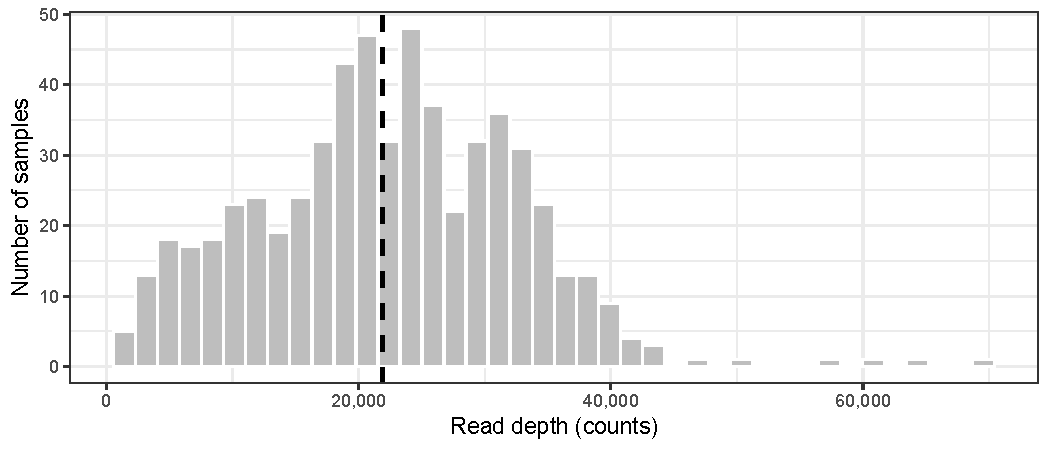
\includegraphics[width=\textwidth]{../ch07_application/figures/01_overview/thesis_seq_depth-1.pdf}
\caption{\textbf{Per-sample sequencing depth.} Distribution of sequencing depth across samples in the reduced PASTURE data set. The histogram shows the number of samples per read depth, with a median library size of 21{,}914 reads (dashed line) and a range from 1{,}456 to 69{,}556 reads.}
\label{fig:7app:library_size}
\end{figure}

%====================================
\subsection{Taxonomic aggregation and prevalence filtering}
\label{sec:7app:taxonomic_aggregation_filtering}
%====================================

After restricting the data set to the reduced analysis subset, ASVs with zero total counts within this subset are removed. Such ASVs occur only in samples outside the reduced data set and therefore do not provide information for the analyses in this chapter. At the ASV level, the original data set contains $p = 5834$ taxa, of which $p = 2045$ have at least one positive count in the reduced analysis subset.

The prevalence--abundance relationship at ASV level is shown in Figure~\ref{fig:7app:prevalence_abundance}. Most ASVs are observed in only a small fraction of samples, whereas a small number of taxa are both highly prevalent and abundant. This pattern is typical for infant gut microbiome data and illustrates why taxonomic aggregation and prevalence filtering are relevant preprocessing steps for the subsequent analyses. Low-prevalence taxa contribute strongly to sparsity, increase the influence of zero handling, and provide limited information for stable statistical estimation.

\begin{figure}[H]
\centering
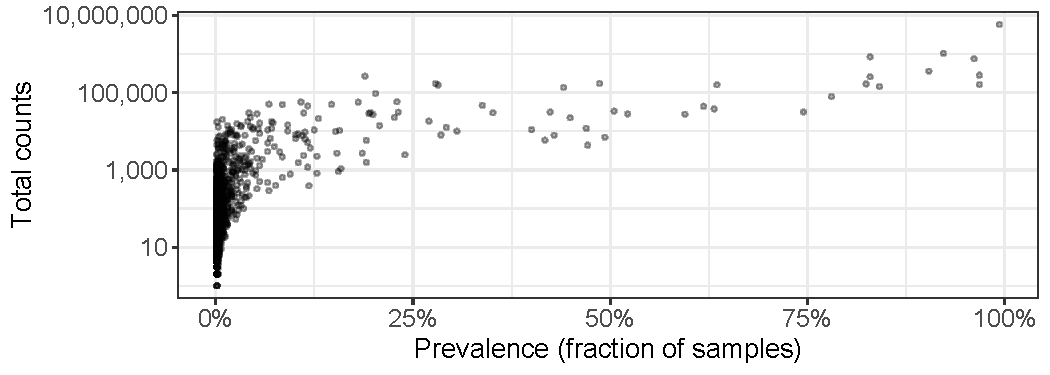
\includegraphics[width=\textwidth]{../ch07_application/figures/02_filtering/thesis_prevalence_asv-1.pdf}
\caption{\textbf{Prevalence--abundance relationship.} Each dot represents an amplicon sequence variant (ASV). The x-axis shows the proportion of samples in which the ASV is observed, i.e. has non-zero counts, and the y-axis shows the total number of counts across all samples. The y-axis is displayed on a log scale, while the axis labels correspond to the original count values.}
\label{fig:7app:prevalence_abundance}
\end{figure}

Table~\ref{tab:7app:taxonomic_overview} summarizes the number of taxa and the proportion of zero entries obtained at different taxonomic levels after restricting the data to the reduced analysis subset. As expected, aggregation to higher taxonomic ranks reduces both dimensionality and sparsity. However, aggregation also changes the biological and statistical target: an ASV-level feature represents an individual sequence variant, whereas a genus-level feature represents the combined signal of all ASVs assigned to the same genus.

\begin{table}[!ht]
\centering
\caption{\textbf{Number of taxa across taxonomic levels.} Number of taxa and proportion of zero entries obtained at different taxonomic levels after restricting the data to the reduced analysis subset and removing taxa with zero total counts.}
\label{tab:7app:taxonomic_overview}
\vspace{0.5em}
\begin{tabular}{lrr}
\toprule
Taxonomic level & Number of taxa & Zero entries (\%) \\
\midrule
ASV & 2045 & 98.2 \\
Genus & 235 & 89.7 \\
Family & 91 & 80.8 \\
Order & 52 & 73.8 \\
Class & 16 & 55.4 \\
Phylum & 10 & 54.9 \\
\bottomrule
\end{tabular}
\end{table}

All analyses in this application chapter are conducted at genus level unless stated otherwise. The ASV count table is therefore aggregated by summing counts over ASVs assigned to the same genus. The genus level provides a compromise between biological resolution, interpretability, and statistical stability: it is less sparse than the ASV-level table, but still sufficiently resolved to describe differences in the early-life gut microbiome at an interpretable taxonomic scale. The resulting unfiltered genus-level table contains $p = 235$ genera and is used for descriptive genus-level summaries and for the alpha diversity analysis.

At the genus level, the data are dominated by a small number of highly abundant taxa (Table~\ref{tab:7app:top_genera}). The most abundant genus is \emph{Bifidobacterium}, which is present in all samples and accounts for a large fraction of the mean relative abundance. Other prevalent genera include \emph{Escherichia-Shigella}, \emph{Streptococcus}, \emph{Bacteroides}, \emph{Enterococcus}, \emph{Blautia}, and a genus of the \emph{Enterobacteriaceae} family. These observations are consistent with previous studies on early-life gut microbiome development \citep{favier2003development}.

\begin{table}[!ht]
\centering
\caption{\textbf{Most abundant genera.} Top 10 most abundant genera in the reduced PASTURE data set ranked by mean relative abundance across samples before prevalence filtering. For each genus, the mean relative abundance, defined as the average proportion of counts assigned to a genus across samples, and the prevalence, defined as the proportion of samples in which the genus is observed, are reported.}
\label{tab:7app:top_genera}
\vspace{0.5em}
\begin{tabular}{lrr}
\toprule
Genus & Mean rel. abundance (\%) & Prevalence (\%) \\
\midrule
\emph{Bifidobacterium} & 63.8 & 100.0 \\
\emph{Escherichia-Shigella} & 5.9 & 97.3 \\
\emph{Streptococcus} & 4.9 & 99.3 \\
\emph{Bacteroides} & 4.6 & 90.5 \\
\emph{Enterobacteriaceae(F)} & 2.9 & 73.8 \\
\emph{Enterococcus} & 2.8 & 90.2 \\
\emph{[Ruminococcus] gnavus group} & 2.3 & 97.6 \\
\emph{Blautia} & 2.0 & 99.2 \\
\emph{Collinsella} & 1.3 & 85.0 \\
\emph{Lactobacillus} & 1.3 & 54.2 \\
\bottomrule
\end{tabular}
\end{table}

For all analyses except alpha diversity, an additional prevalence filter is applied at genus level. Genera observed in less than 1\% of the samples are removed. This threshold removes genera with too few non-zero observations to support stable statistical estimation, while retaining a broad genus-level representation of the microbiome. Table~\ref{tab:7app:prevalence_filtering} summarizes the effect of different prevalence thresholds on the number of retained genera and the proportion of zero entries. The 1\% filter reduces the number of genera from 235 to 117 and decreases the proportion of zero entries from 89.7\% to 79.6\%. More stringent thresholds would further reduce sparsity, but would also remove a large fraction of genera and thereby substantially narrow the taxonomic scope of the subsequent analyses.

\begin{table}[!ht]
\centering
\caption{\textbf{Effect of prevalence filtering on the genus-level count table.} Number of retained genera and proportion of zero entries for different prevalence thresholds. Prevalence is defined as the proportion of samples in which a genus has positive counts.}
\label{tab:7app:prevalence_filtering}
\vspace{0.5em}
\begin{tabular}{lrr}
\toprule
Prevalence threshold & Number of genera & Zero entries (\%) \\
\midrule
No prevalence filtering & 235 & 89.7 \\
$\geq 1\%$ of samples & 117 & 79.6 \\
$\geq 5\%$ of samples & 58 & 61.3 \\
$\geq 10\%$ of samples & 41 & 48.4 \\
$\geq 20\%$ of samples & 31 & 36.4 \\
\bottomrule
\end{tabular}
\end{table}

Although the 1\% prevalence filter reduces the overall proportion of zero entries, the retained genus-level table remains strongly sparse. Figure~\ref{fig:7app:zero_fraction_filtered_genera} shows the distribution of zero fractions across the 117 retained genera. Many genera are still absent from a large majority of samples, with a pronounced accumulation of zero fractions above 90\%. Thus, the filter removes only the most extremely rare genera and does not eliminate the need for zero-aware preprocessing and analysis methods in the subsequent sections.


\begin{figure}[!htb]
\centering
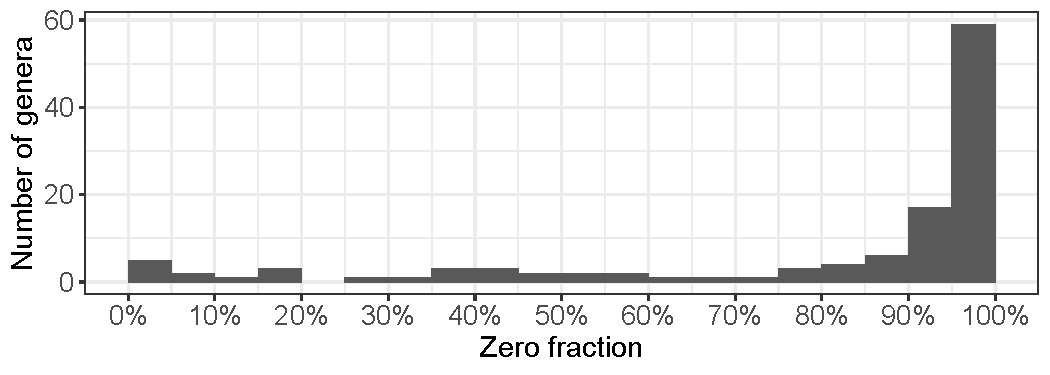
\includegraphics[width=0.75\textwidth]{../ch07_application/figures/02_filtering/thesis_zero_fraction_plot-1.pdf}
\caption{\textbf{Distribution of zero fractions after 1\% prevalence filtering.} The histogram shows, for each of the 117 genera retained after applying the 1\% prevalence filter, the proportion of samples with zero counts.}
\label{fig:7app:zero_fraction_filtered_genera}
\end{figure}

%====================================
\subsection{Default data set for downstream analyses}
\label{sec:7app:default_data}
%====================================

The downstream analyses in this chapter use the genus-level representation introduced in Section~\ref{sec:7app:taxonomic_aggregation_filtering}. Unless stated otherwise, analyses after the within-sample diversity section are based on the $1\%$ prevalence-filtered genus-level count table with $117$ retained genera. This table is referred to as the default analysis data set in the following sections. The main exception is the within-sample diversity analysis, which is computed before prevalence filtering because removing low-prevalence genera would directly change the target of richness and diversity estimation. If another taxonomic table, sample subset, or data transformation is used in a later section, this is stated explicitly.

The default analysis data set is represented on different scales depending on the analysis target. The choice of representation follows the preprocessing strategy summarized in Section~\ref{sec:2micro:preprocessing_choices_thesis} and is implemented here for the reduced PASTURE data set. Relative abundances are used for descriptive summaries and for analyses based on Bray--Curtis dissimilarity, because they provide an interpretable representation of the observed sample composition after adjustment for library size. For analyses requiring a log-ratio representation, counts are first converted to relative abundances, zeros are replaced by multiplicative replacement, and the resulting strictly positive compositions are transformed using the centered log-ratio transformation. This CLR representation is used for Aitchison distances, regression models for compositional responses, compositional equivalence, exploratory CLR-coordinate visualizations, the CLR-based part of the differential distribution analysis, and network analyses.

Analyses based on EBF duration require an additional distinction. When EBF duration is used as the main binary grouping variable, samples with missing EBF duration and the three samples in the sparse 1-month EBF category are excluded from the corresponding two-group comparison. The resulting contrast compares children without EBF ($n=179$) with children with EBF duration $\ge 2$ months ($n=375$). This exclusion is applied only in analyses that explicitly use this binary EBF contrast and is not a general filtering step applied to the entire chapter. To improve readability, the EBF duration $\geq 2$ months group is referred to as the ``EBF'' group and the EBF duration $=0$ months group as the ``non-EBF'' group in the following comparative analyses.

Figure~\ref{fig:7app:rel-clr-histogram-comparison} illustrates the effect of the relative-abundance and CLR representations for the most abundant genera. The left panels show relative abundances, which are bounded between zero and one and are often strongly concentrated near zero for sparse genera. The right panels show the corresponding CLR coordinates after multiplicative replacement. These values are no longer abundances in the original sense, but log-ratio coordinates relative to the sample-wise geometric mean. Originally zero observations are mapped to low CLR values whose location depends on the replacement rule and on the remaining composition of the same sample. The comparison emphasizes that downstream analyses based on CLR-transformed data operate in a different coordinate system and should be interpreted in terms of relative log-ratios rather than absolute microbial abundance.

\begin{figure}[!htb]
\centering
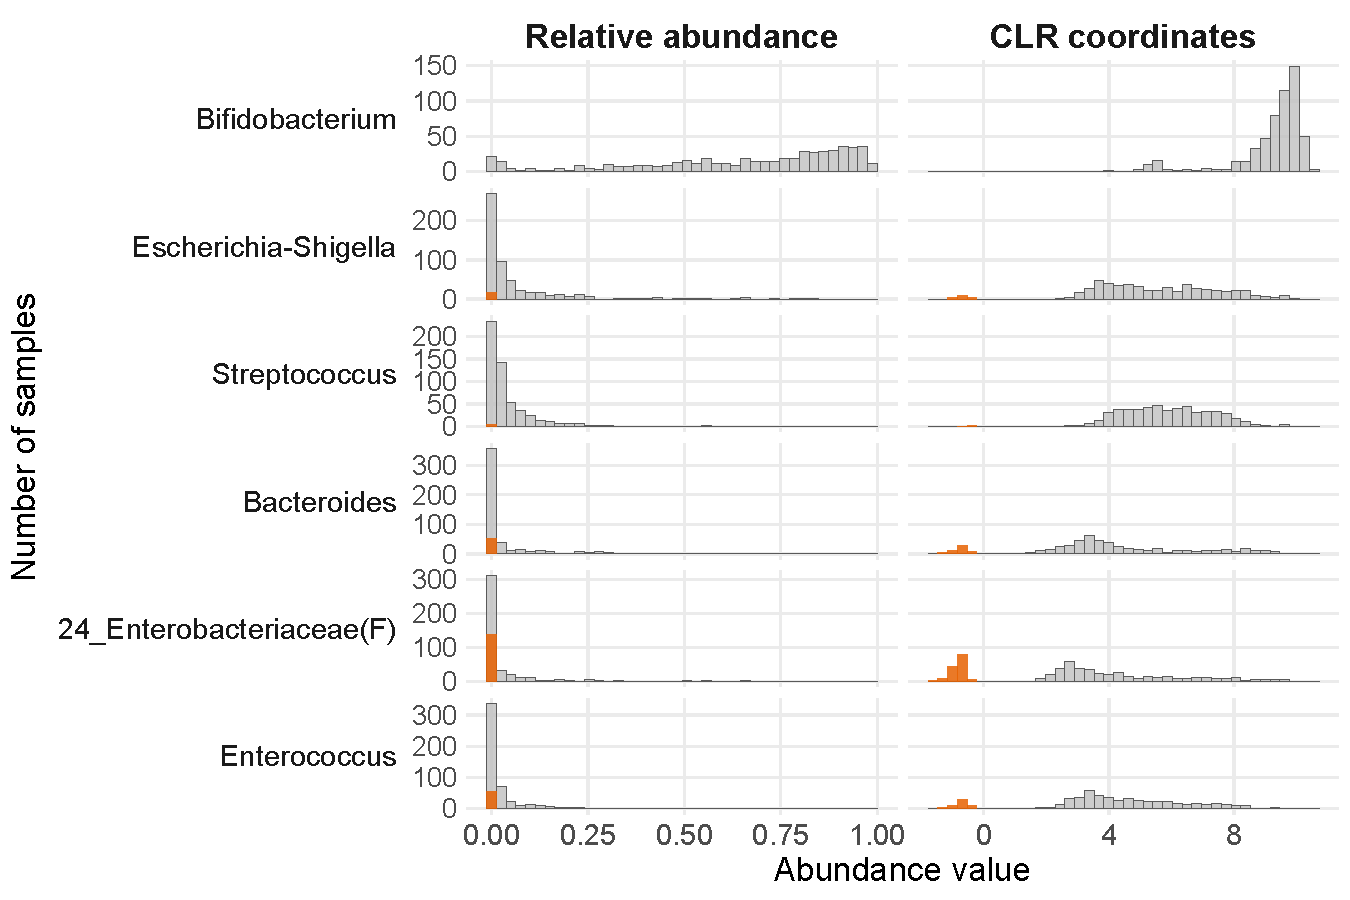
\includegraphics[width=\textwidth]{../ch07_application/figures/07_exploration/thesis_rel_to_clr_histogram_comparison-1.pdf}
\caption{\textbf{Relative abundances and CLR coordinates for the most abundant genera.} The left panels show relative abundances after total sum scaling, and the right panels show CLR coordinates after multiplicative replacement of zeros. Orange bars indicate samples in which the corresponding genus was originally absent before zero replacement. The figure illustrates that CLR transformation changes the coordinate representation of the data: values are interpreted as log-ratios relative to the sample-wise geometric mean and not as absolute abundances.}
\label{fig:7app:rel-clr-histogram-comparison}
\end{figure}

Taken together, the reduced data set retains the central statistical characteristics of microbiome sequencing data: unequal library sizes, compositional constraints, sparsity, and strong heterogeneity in taxon prevalence and abundance. The default genus-level analysis data set provides a common basis for the following sections, while deviations in taxonomic resolution, sample subset, or data representation are stated where they are required by the respective method. This structure supports a coherent analysis workflow from community-level exploration to feature-level testing and network-based comparison.

%%%%%%%%%%%%%%%%%%%%%%%%%%%%%%%%%%%%%
\section{Within-sample diversity}
\label{sec:7app:alpha}
%%%%%%%%%%%%%%%%%%%%%%%%%%%%%%%%%%%%%

Within-sample diversity, commonly referred to as \emph{alpha diversity}, provides a first aggregated view of microbial community structure by reducing each sample-specific taxon profile to a scalar summary. As introduced in Section~\ref{sec:3community:within_sample_div}, it can be characterized by richness, which reflects the number of taxa present in a sample, and by diversity indices such as Shannon entropy and the Gini--Simpson index, which additionally account for the distribution of abundances across taxa.

In this section, within-sample diversity in the reduced PASTURE data set is analyzed using the model-based estimators described in Chapter~\ref{ch:community}. We first compare classical and model-based richness estimates and assess their dependence on sequencing depth. We then investigate differences in diversity across cohort variables using rank-based tests.
To assess the robustness of these findings, asymptotic and permutation-based $p$-values are compared, including $p$-value refinement with the \texttt{permApprox} framework introduced in Chapter~\ref{ch:permapprox}. Finally, regression-based diversity models are used to incorporate covariates directly into the diversity estimation framework and to compare adjusted effects with the unadjusted group-wise analyses.

%====================================
\subsection{Analysis data}
\label{sec:7app:alpha:data}
%====================================

As stated in Section~\ref{sec:7app:default_data}, within-sample diversity is the main analysis in this chapter that is computed before prevalence filtering. All analyses in this section are therefore based on the unfiltered genus-level count table introduced in Section~\ref{sec:7app:taxonomic_aggregation_filtering}, comprising $592$ samples and $235$ genera. The additional $1\%$ prevalence filter used as the default in later sections is not applied here, because removing low-prevalence genera would directly change the target of richness and diversity estimation.

Although within-sample diversity is often computed at the ASV level, the analysis is performed at the genus level to maintain the taxonomic resolution used throughout the application chapter and to reduce the computational burden of model-based diversity estimation. The exploratory group-wise analyses consider all cohort variables summarized in Section~\ref{sec:7app:data}, including country, sex, mode of delivery, breastfeeding-related variables, prenatal smoking, and number of siblings.

As discussed in Chapter~\ref{ch:community}, rarefaction is not used as a preprocessing step. Instead, richness and diversity are estimated using the model-based approaches proposed by \citet{willis2018divnet,willis2022breakaway}, which account for sampling effort and uncertainty due to unobserved taxa. Consequently, no additional rarefaction, normalization, or prevalence filtering is applied to the count data in this section.

%====================================
\subsection{Comparison of richness estimators}
\label{sec:7app:alpha:rich_comparison}
%====================================

We compare three conceptually distinct notions of richness: (i) observed richness, defined as the number of detected genera per sample, (ii) sample-wise richness estimates obtained using the \texttt{breakaway} package \citep{willis2022breakaway} without covariates, and (iii) model-based richness predictions with \texttt{breakaway}, which are obtained from a regression model that incorporates covariates.

Observed richness is a purely empirical quantity that counts the number of non-zero taxa in each sample. As such, it is directly influenced by sequencing depth and does not account for unobserved low-abundance taxa (cf. Section~\ref{sec:3community:within:richness}). In contrast, \texttt{breakaway} estimates the total richness of a sample by extrapolating from the frequency count table, thereby correcting for taxa that are present but not observed. Importantly, when applied without covariates, \texttt{breakaway} produces \emph{independent, sample-wise estimates} that do not borrow information across samples.

Figure~\ref{fig:7app:alpha_obs_vs_breakaway} (left panel) compares observed richness to \texttt{breakaway} estimates obtained without covariates. The two measures are almost perfectly linearly related, indicating that the correction for unobserved taxa is negligible in this data set. Consequently, \texttt{breakaway} does not substantially alter the ranking of samples compared to observed richness. Similar results are obtained at the ASV level (not shown), suggesting that this behavior is not driven by the level of taxonomic aggregation.

\begin{figure}[H]
    \centering
    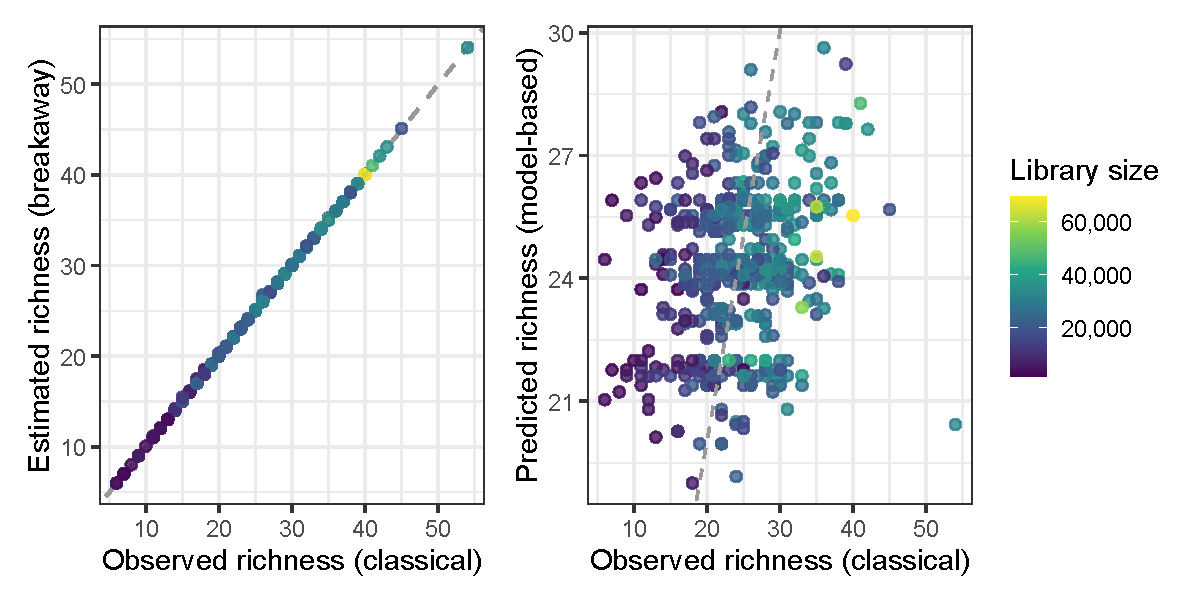
\includegraphics[width=\textwidth]{../ch07_application/figures/03_alpha_diversity/thesis_observed_vs_predicted_richness_libsize_combined-1.pdf}
    \caption{\textbf{Comparison of observed and model-based richness.} Left: observed richness versus \texttt{breakaway} estimates obtained without covariates. Right: observed richness versus model-based predicted richness obtained from a \texttt{breakaway} regression model with covariates. Points are colored by library size.}
    \label{fig:7app:alpha_obs_vs_breakaway}
\end{figure}

To understand this behavior, it is instructive to examine the frequency count structure underlying the breakaway estimator. Breakaway relies on the number of rare taxa, in particular singletons (taxa observed exactly once), to estimate the number of unobserved taxa. Figure~\ref{fig:7app:alpha_frequency_counts} shows the mean number of taxa per sample as a function of their observed frequency. Notably, the number of singletons is exactly zero across samples. As a consequence, the ratio-based estimators used by breakaway collapse to the observed richness, since the observed frequency count spectrum provides little information for estimating unobserved taxa. This explains the near identity between observed and breakaway richness in Figure~\ref{fig:7app:alpha_obs_vs_breakaway}.

The absence of singletons was observed not only at the genus level but also at the ASV level (not shown). Since singleton ASVs are commonly removed during denoising and error-correction procedures in amplicon sequence processing pipelines such as DADA2, this pattern is likely a consequence of the preprocessing applied to the sequencing data prior to the present analysis. As a result, the frequency count spectrum contains little information for extrapolating beyond the observed richness.

\begin{figure}[H]
    \centering
    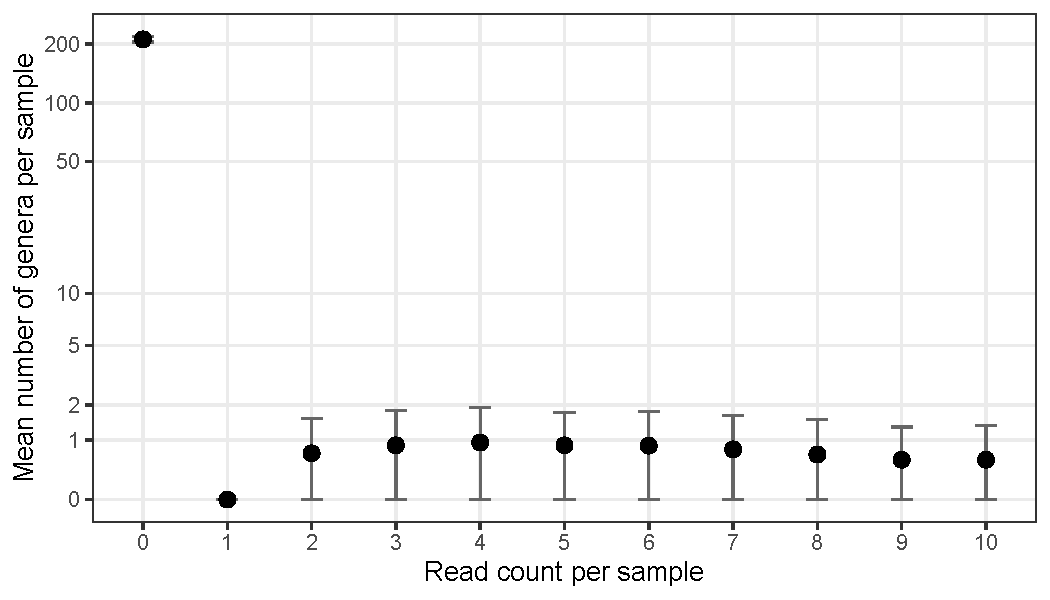
\includegraphics[width=0.9\textwidth]{../ch07_application/figures/03_alpha_diversity/thesis_freq_spectrum_genus-1.pdf}
    \caption{\textbf{Frequency count spectrum at genus level.} Mean number of genera per sample as a function of their observed frequency (read count per sample). Error bars indicate variability across samples. The absence of singletons (genera with one read count per sample) implies that no information about unobserved taxa is available for ratio-based richness estimation.}
    \label{fig:7app:alpha_frequency_counts}
\end{figure}

In a second step, richness is modeled as a function of covariates using the \texttt{betta()} function from \texttt{breakaway}. In contrast to the sample-wise estimation described above, this model is fitted across samples and yields \emph{predicted richness values} conditional on the covariates. These values therefore represent fitted expectations under the model rather than direct estimates of sample-specific richness.

The effect of this modeling step is illustrated in Figure~\ref{fig:7app:alpha_obs_vs_breakaway} (right panel). Compared to the near one-to-one relationship in the left panel, the predicted richness values exhibit substantially reduced variability and a compressed range. This behavior reflects the fact that regression-based predictions are shrunk towards the fitted mean structure and primarily capture systematic variation explained by the covariates. As a consequence, they no longer preserve the original between-sample variability present in the data.

This distinction is crucial for interpretation. While \texttt{breakaway} without covariates aims to estimate the underlying richness of each individual sample, the regression model targets the expected richness given the covariates. The resulting quantities therefore answer different statistical questions: one is a per-sample estimate, the other a model-based prediction.

For comparative analyses, this difference has direct methodological implications. Using model-based predicted richness for group comparisons would lead to circular inference, as the grouping variable is already used in the model fitting step. Any subsequent test would therefore assess differences that have been, at least partially, imposed by the model itself. To avoid this double use of information, all statistical comparisons in the following are based on the sample-wise richness estimates rather than on model-based predictions.

Model-based predictions nevertheless serve an important role for visualization and interpretation of covariate effects. They provide a smoothed representation of systematic trends and can help disentangle the influence of multiple covariates. However, they are not suitable as input for hypothesis testing in this setting.

Taken together, these results highlight two key points. First, at the genus level, the correction for unobserved taxa provided by breakaway has only a minor effect when applied without covariates. This is not merely an empirical observation but can be directly explained by the absence of singletons in the data, which eliminates the information required for extrapolation. Second, regression-based modeling substantially alters the scale and variability of richness by imposing a covariate-driven structure, which makes the resulting predictions fundamentally different from sample-wise richness estimates.

%====================================
\subsection{Within-sample diversity across cohort variables}
\label{sec:7app:alpha:diversity_measures}
%====================================

In addition to richness, we considered two complementary diversity indices that account for the distribution of abundances within samples: the Shannon index and the Gini--Simpson index. Both measures were estimated using the \texttt{DivNet} framework described in Section~\ref{sec:3community:within_sample_div}, which provides model-based diversity estimates while accounting for compositional dependencies among taxa. The \texttt{divnet()} function from the \texttt{DivNet} package \citep{willis2018divnet} was applied to the genus-level count table to estimate Shannon and Simpson diversity. For the log-ratio representation underlying the model, \textit{Bifidobacterium} was used as the reference taxon, as it exhibited 100\% prevalence across all samples. The Simpson index returned by \texttt{DivNet} was transformed into the Gini--Simpson index by computing $1 - \text{Simpson}$. While the Simpson index measures concentration or dominance, the Gini--Simpson index instead quantifies diversity, with larger values indicating a more even distribution of abundances across taxa.

To investigate whether within-sample diversity differs across cohort variables, we compared richness, Shannon diversity, and the Gini--Simpson index across all covariates available in the reduced data set: Country, Sex, C-section, BF duration, EBF duration, Smoking, and Siblings (Table~\ref{tab:7app:sample_characteristics}). For EBF duration, the three samples in the one-month category were excluded from the group comparison, because this category was too small to support an informative comparison. For each variable and diversity measure, an overall group effect was first assessed using a Kruskal--Wallis test based on its standard asymptotic chi-squared approximation. If the resulting $p$-value was significant at the $\alpha = 0.05$ level and the variable had more than two groups, pairwise comparisons between groups were additionally performed using asymptotic Wilcoxon rank-sum tests.

The resulting overall test statistics and asymptotic $p$-values are summarized in Table~\ref{tab:7app:perm_results}. Pairwise Wilcoxon results are not included in the table, but significant pairwise comparisons are annotated in the corresponding figures. Figure~\ref{fig:7app:alpha_div_excl_bf} shows the selected EBF duration comparison, while additional visualizations for the remaining cohort variables are provided in Appendix~\ref{sec:app:7app:alpha_remaining}, and also in the \href{https://github.com/stefpeschel/phd_thesis/tree/main/ch07_application}{\texttt{ch07\_application}} folder of the thesis repository described at the beginning of this chapter. The subsequent subsection evaluates whether the asymptotic $p$-values used for interpretation agree with permutation-based and \texttt{permApprox}-refined $p$-values.

The results indicate that within-sample diversity differs substantially across several cohort variables. In particular, BF duration, EBF duration, Smoking, and Country show significant associations with both diversity indices. In contrast, richness exhibits fewer significant associations and generally weaker effects, consistent with the findings of the previous subsection. Sex and Siblings do not show significant differences for any of the considered measures. For C-section, significant differences are observed for Shannon diversity and the Gini--Simpson index, whereas richness remains non-significant.

Among the considered variables, BF duration and EBF duration show the strongest associations with within-sample diversity, as reflected by the smallest asymptotic $p$-values in Table~\ref{tab:7app:perm_results}. These variables therefore represent promising candidates for further investigation and more detailed group comparisons in the subsequent sections.

For the downstream analyses, we aim to identify a grouping variable with two sufficiently large and balanced groups. In this regard, EBF duration provides a suitable choice. In particular, the comparison between the groups corresponding to no exclusive breastfeeding and at least two months of exclusive breastfeeding yields more balanced group sizes than the corresponding categorization based on BF duration (Table~\ref{tab:7app:sample_characteristics}).

Figure~\ref{fig:7app:alpha_div_excl_bf} shows the corresponding distributions of richness, Shannon diversity, and the Gini--Simpson index across the two EBF duration groups. While richness shows only minor differences between groups, both diversity indices indicate substantially lower diversity for at least two months of exclusive breastfeeding. The effect is particularly pronounced for the Shannon index, where the distributions are clearly shifted between groups. This pattern is in line with previous studies identifying infant feeding mode as a major determinant of early-life gut-microbiome composition and reporting lower gut microbial diversity among exclusively breastfed infants during early infancy \citep{ho2018metaanalysis,ma2020comparison,odiase2023gut}.

\begin{figure}[H]
\centering
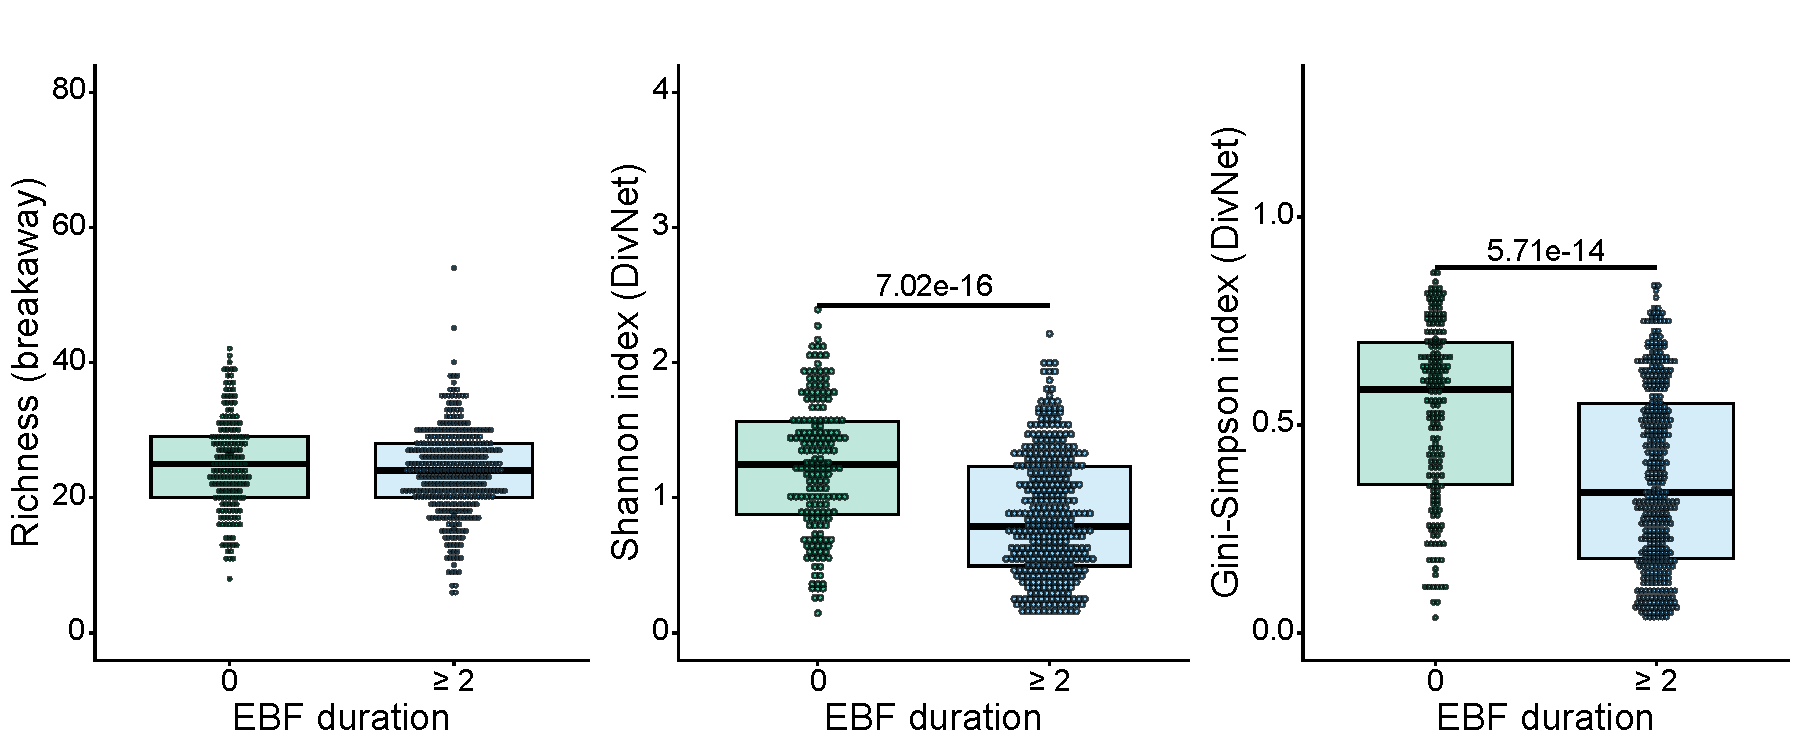
\includegraphics[width=\textwidth]{../ch07_application/figures/03_alpha_diversity/thesis_breast_excl_2m-1.pdf}
\caption{\textbf{Within-sample diversity by EBF duration.} Sample-wise estimates of richness, Shannon diversity, and the Gini--Simpson index for children with no exclusive breastfeeding and children with at least two months of exclusive breastfeeding. Richness was estimated using \texttt{breakaway}; Shannon diversity and the Gini--Simpson index were estimated using \texttt{DivNet}. Reported $p$-values are asymptotic Kruskal--Wallis $p$-values. The one-month category was excluded because it contained only three samples. Sample sizes are 179 for no exclusive breastfeeding and 375 for at least two months of exclusive breastfeeding.}
\label{fig:7app:alpha_div_excl_bf}
\end{figure}

%====================================
\subsection{Permutation-based inference and $p$-value refinement}
\label{sec:7app:alpha:permutation}
%====================================

The previous subsection relied on the standard asymptotic approximation of the Kruskal--Wallis test statistic, where the test statistic is approximated by a chi-squared distribution with degrees of freedom equal to the number of groups minus one. While this approximation is commonly used in practice, its validity may be affected by small or unbalanced group sizes, ties in the data, and deviations from the asymptotic regime. To assess the robustness of the obtained results, we therefore complemented the asymptotic inference by permutation-based testing.

For each cohort variable and diversity measure, the Kruskal--Wallis test statistic was recomputed under random permutations of the group labels to generate an empirical null distribution for the overall group effect. The test statistic was computed directly from the group-wise rank sums using the formulation introduced in Section~\ref{sec:3community:within:testing}. Permutation-based $p$-values were then computed from the number of permuted statistics greater than or equal to the observed statistic using the adjusted estimator in Equation~\eqref{eq:6perm:empirical_pvalue}. The comparison in this subsection focuses on the overall tests reported in Table~\ref{tab:7app:perm_results}. The pairwise Wilcoxon annotations shown in Figure~\ref{fig:7app:alpha_div_excl_bf} and Appendix~\ref{sec:app:7app:alpha_remaining} are based on asymptotic Wilcoxon rank-sum tests.

Although substantially fewer permutations would have been sufficient for the present analysis, we generated $10^6$ permutations for each overall test. In this setting, the computational cost of permutation testing is comparatively small because the within-sample diversity measures are computed only once and each permutation merely requires recomputation of the rank-based test statistic. The large number of permutations therefore provides an opportunity to directly assess how closely the asymptotic $p$-values agree with the empirical permutation distribution over several orders of magnitude.

The resulting $p$-values are summarized in Table~\ref{tab:7app:perm_results}. Overall, the empirical permutation $p$-values closely match the asymptotic $p$-values and typically agree up to the same order of magnitude, even for very small $p$-values. This close agreement provides reassurance that the asymptotic approximation yields similar inferential conclusions in the present setting. Thus, permutation-based inference does not appear to be necessary for obtaining materially different conclusions for these overall diversity tests.

Nevertheless, this setting provides a useful opportunity to evaluate the behavior of the \texttt{permApprox} framework in a low-dimensional setting. The empirical permutation $p$-values are bounded below by about $10^{-6}$ due to the finite number of permutations, whereas \texttt{permApprox} further refines the tail probabilities by fitting a generalized Pareto distribution to the upper tail of the permutation distribution under the support constraint proposed in Section~\ref{sec:6perm:constraint}. The refinement was performed using the default settings of the package, except that the number of starting exceedances was reduced to 5000 permutations (corresponding to 0.5\% of all permutations) to reduce runtime.

The refined $p$-values shown in the rightmost columns of Table~\ref{tab:7app:perm_results} remain close to the asymptotic $p$-values and are slightly more conservative for extremely small $p$-values. This behavior is desirable, as it avoids overly optimistic tail extrapolation while still extending the resolution beyond the empirical permutation limit. In the present analysis, the refinement does not alter the resulting significance decisions, which is expected given the close agreement between asymptotic and empirical permutation inference.

These results illustrate an important practical aspect of the proposed methodology. In the present setting, the asymptotic approximation already provides reliable inference, likely due to the comparatively large sample size and the absence of severe violations of the assumptions underlying the rank-based tests. In settings where these assumptions are less well satisfied, for example in the presence of smaller sample sizes, strongly imbalanced groups, or more irregular null distributions, permutation-based inference provides a robust alternative that does not rely on parametric approximations. In such cases, \texttt{permApprox} becomes particularly useful by refining extremely small empirical permutation $p$-values beyond the finite permutation resolution. As will be demonstrated in the subsequent sections, this refinement becomes increasingly relevant in more complex testing scenarios involving large-scale multiple testing and computationally expensive permutation procedures.


\begin{table}[H]
\centering
\caption{Kruskal--Wallis test results for within-sample diversity across cohort variables. $H$ is the Kruskal--Wallis test statistic. Richness was estimated using \texttt{breakaway}; Shannon and Gini--Simpson diversity were estimated using \texttt{DivNet}. $p$ (asymptotic) denotes the chi-squared approximation used for the exploratory interpretation; $p$ (permutation) denotes empirical permutation $p$-values based on $10^6$ permutations; $p$ (GPD-refined) denotes $p$-values obtained with \texttt{permApprox} for small empirical permutation $p$-values. $p$-values are rounded and shown in scientific notation with two digits after the decimal point. The smallest attainable empirical permutation $p$-value is $1/(10^6+1)$, which is displayed as $1.00\mathrm{e}{-06}$ after rounding.}
\label{tab:7app:perm_results}
\centering
\begin{threeparttable}
\begin{tabular}[t]{l@{\hspace{4em}}rlll}
\toprule
Measure & $H$ & $p$ (asymptotic) & $p$ (permutation) & $p$ (GPD-refined)\\
\midrule
\addlinespace[0.3em]
\multicolumn{5}{l}{\textbf{Country}}\\
\hspace{1em}Richness & 31.57 & 1.40e-07$^{***}$ & 1.00e-06$^{***}$ & 1.99e-07$^{***}$\\
\hspace{1em}Shannon & 40.06 & 2.00e-09$^{***}$ & 1.00e-06$^{***}$ & 3.01e-09$^{***}$\\
\hspace{1em}Gini-Simpson & 39.88 & 2.19e-09$^{***}$ & 1.00e-06$^{***}$ & 4.89e-09$^{***}$\\
\addlinespace[0.3em]
\multicolumn{5}{l}{\textbf{Sex}}\\
\hspace{1em}Richness & 1.79 & 1.80e-01 & 1.77e-01 & 1.77e-01\\
\hspace{1em}Shannon & 1.85 & 1.73e-01 & 1.72e-01 & 1.72e-01\\
\hspace{1em}Gini-Simpson & 2.10 & 1.47e-01 & 1.49e-01 & 1.49e-01\\
\addlinespace[0.3em]
\multicolumn{5}{l}{\textbf{C-section}}\\
\hspace{1em}Richness & 0.33 & 5.64e-01 & 5.64e-01 & 5.64e-01\\
\hspace{1em}Shannon & 4.86 & 2.74e-02$^{*}$ & 2.54e-02$^{*}$ & 2.50e-02$^{*}$\\
\hspace{1em}Gini-Simpson & 5.73 & 1.67e-02$^{*}$ & 1.35e-02$^{*}$ & 1.43e-02$^{*}$\\
\addlinespace[0.3em]
\multicolumn{5}{l}{\textbf{BF duration}}\\
\hspace{1em}Richness & 7.69 & 2.14e-02$^{*}$ & 2.12e-02$^{*}$ & 2.12e-02$^{*}$\\
\hspace{1em}Shannon & 83.47 & 7.51e-19$^{***}$ & 1.00e-06$^{***}$ & 1.44e-17$^{***}$\\
\hspace{1em}Gini-Simpson & 73.49 & 1.10e-16$^{***}$ & 1.00e-06$^{***}$ & 4.69e-15$^{***}$\\
\addlinespace[0.3em]
\multicolumn{5}{l}{\textbf{EBF duration}}\\
\hspace{1em}Richness & 2.73 & 9.84e-02$^{.}$ & 9.84e-02$^{.}$ & 9.84e-02$^{.}$\\
\hspace{1em}Shannon & 65.13 & 7.02e-16$^{***}$ & 1.00e-06$^{***}$ & 5.18e-14$^{***}$\\
\hspace{1em}Gini-Simpson & 56.47 & 5.71e-14$^{***}$ & 1.00e-06$^{***}$ & 5.04e-14$^{***}$\\
\addlinespace[0.3em]
\multicolumn{5}{l}{\textbf{Smoking}}\\
\hspace{1em}Richness & 3.95 & 4.70e-02$^{*}$ & 4.69e-02$^{*}$ & 4.69e-02$^{*}$\\
\hspace{1em}Shannon & 18.81 & 1.45e-05$^{***}$ & 1.30e-05$^{***}$ & 1.01e-05$^{***}$\\
\hspace{1em}Gini-Simpson & 18.08 & 2.12e-05$^{***}$ & 1.60e-05$^{***}$ & 1.47e-05$^{***}$\\
\addlinespace[0.3em]
\multicolumn{5}{l}{\textbf{Siblings}}\\
\hspace{1em}Richness & 1.41 & 4.94e-01 & 4.97e-01 & 4.97e-01\\
\hspace{1em}Shannon & 2.66 & 2.64e-01 & 2.61e-01 & 2.61e-01\\
\hspace{1em}Gini-Simpson & 3.04 & 2.18e-01 & 2.20e-01 & 2.20e-01\\
\bottomrule
\end{tabular}
\begin{tablenotes}
\item $^{***}:p<0.001$; $^{**}:p<0.01$; $^{*}:p<0.05$; $^{\textbf{.}}:p<0.1$.
\end{tablenotes}
\end{threeparttable}
\end{table}

%====================================
\subsection{Regression-based within-sample diversity analysis}
\label{sec:7app:alpha:regression}
%====================================

As a complementary approach to the group-wise comparisons, we fitted regression-based alpha diversity models using the \texttt{betta()} function from the \texttt{breakaway} package. The same modeling framework was already used in Section~\ref{sec:7app:alpha:rich_comparison} to obtain covariate-based richness predictions. Here, we focus on the regression coefficients rather than the predicted values, since the aim is to assess which covariates remain associated with alpha diversity when all variables are considered jointly.

The \texttt{betta()} function takes diversity estimates together with their estimated standard errors as input and fits a regression model that accounts for uncertainty in the estimated response. We applied this approach separately to richness, Shannon diversity, and the Gini--Simpson index. For richness, we used the estimates and standard errors obtained from \texttt{breakaway}; for Shannon diversity and the Gini--Simpson index, we used the estimates and standard errors obtained from \texttt{DivNet}. The model included all covariates considered in the group-wise analyses, namely country, sex, mode of delivery, breastfeeding duration, exclusive breastfeeding duration, prenatal smoking, and number of siblings. Samples with missing values in any of these covariates were excluded from the regression analysis.

Figure~\ref{fig:7app:alpha_betta} summarizes the resulting coefficient estimates and corresponding 95\% confidence intervals. For categorical variables with more than two levels, the first category was used as reference level. Positive coefficients indicate higher expected diversity compared to the reference category, whereas negative coefficients indicate lower expected diversity after adjustment for the remaining covariates.

\begin{figure}[H]
    \centering
    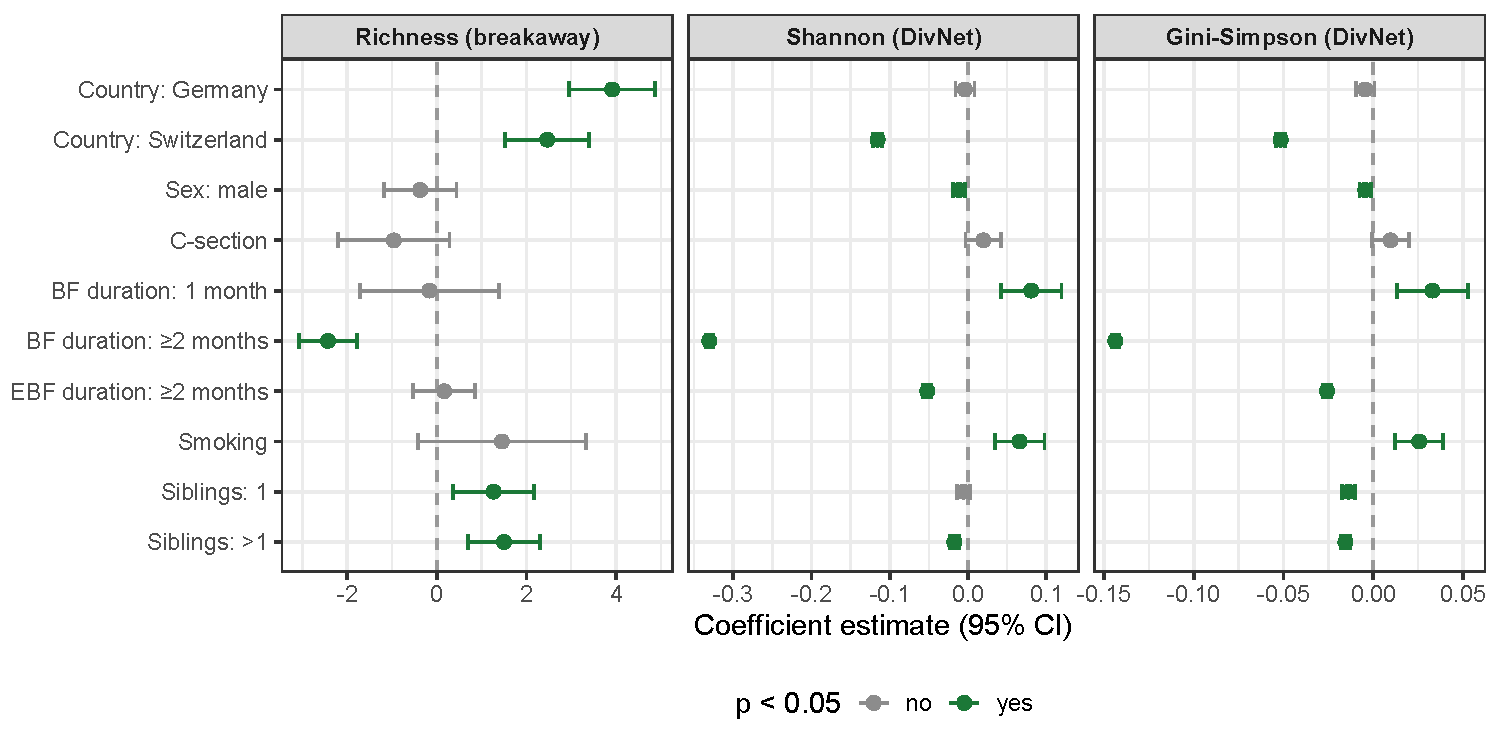
\includegraphics[width=\textwidth]{../ch07_application/figures/03_alpha_diversity/thesis_betta_forest_combined-1.pdf}
    \caption{Regression coefficients and corresponding 95\% confidence intervals obtained from the \texttt{betta()} models for richness, Shannon diversity, and the Gini--Simpson index. Green points indicate coefficients with $p < 0.05$.}
    \label{fig:7app:alpha_betta}
\end{figure}

Overall, the regression-based results are largely consistent with the group-wise comparisons summarized in Table~\ref{tab:7app:perm_results}. Breastfeeding-related variables, Smoking, and Country remain associated with alpha diversity after covariate adjustment. In particular, BF duration $\ge2$ months is associated with substantially lower richness, Shannon diversity, and Gini--Simpson diversity. EBF duration $\ge2$ months is also associated with lower Shannon and Gini--Simpson diversity, whereas its coefficient for richness is close to zero and not significant. This agrees with the group-wise comparisons, where EBF duration showed strong differences in diversity indices but not in richness. Because the two BF variables are closely related, the corresponding regression coefficients should be interpreted as conditional associations within the joint model rather than as independent marginal effects.

For Country, the regression model confirms differences in within-sample diversity, but the direction and magnitude depend on the measure considered. Compared to Austria (the reference country), Germany and Switzerland show higher richness, whereas Switzerland shows lower Shannon and Gini--Simpson diversity. This indicates that differences in richness and evenness do not necessarily point in the same direction, again emphasizing the importance of considering multiple diversity measures.

One notable discrepancy concerns the effect of C-section. In the marginal Kruskal--Wallis tests, both Shannon diversity and the Gini--Simpson index showed significant differences between delivery modes. In contrast, the corresponding regression coefficients are close to zero and no longer statistically significant.

To investigate this discrepancy further, Figure~\ref{fig:7app:alpha_csection_bf} compares BF duration distributions between delivery modes and additionally stratifies Shannon diversity by both variables. The left panel shows that vaginally delivered infants are more frequently represented in the long BF category, which is associated with lower diversity. The stratified boxplots in the right panel indicate that within BF strata, differences between delivery modes are substantially reduced, especially in the ``$\ge$ 2 months'' group, which contains the majority of the samples. This suggests that the apparent delivery mode effect observed in the unconditioned group comparisons is at least partly explained by differences in BF behavior.

This comparison illustrates the different targets of the two inferential strategies. The Kruskal--Wallis test assesses marginal group differences separately for each covariate, whereas the \texttt{betta()} models estimate associations conditioned on the remaining variables. The two approaches therefore answer related but not identical questions. In the present analysis, they lead to largely consistent conclusions, with the exception of delivery mode, where the regression model suggests that the marginal association is confounded by breast feeding duration.

\begin{figure}[H]
	\centering
	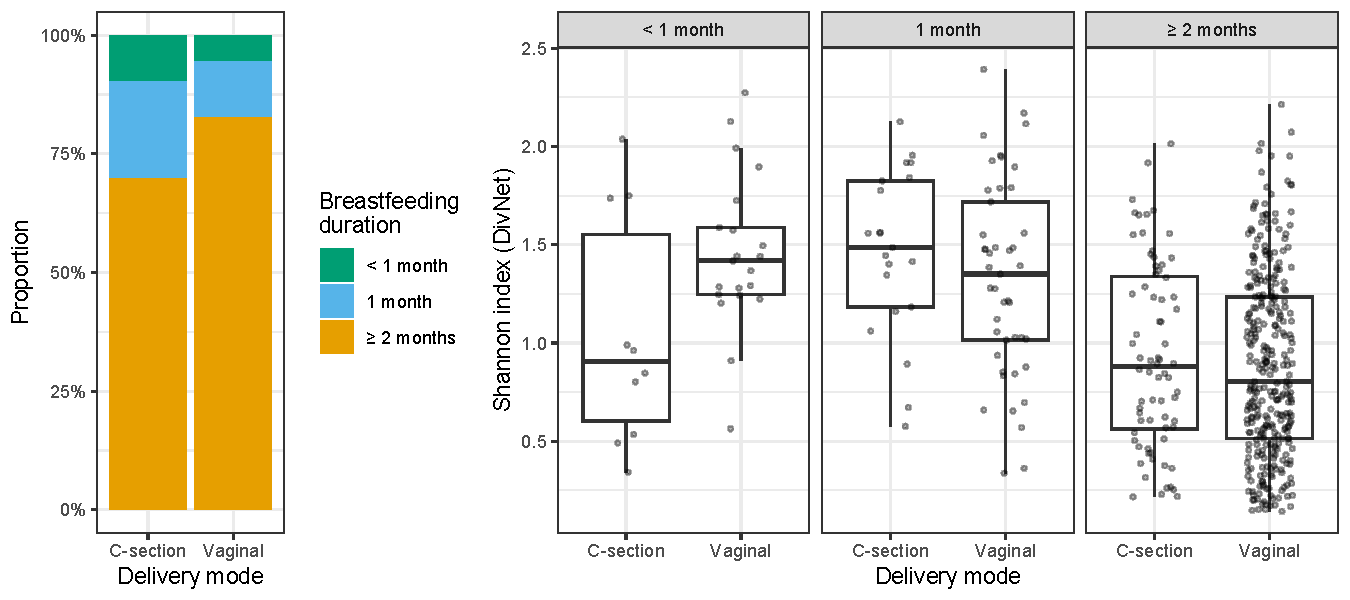
\includegraphics[width=\textwidth]{../ch07_application/figures/03_alpha_diversity/thesis_cesarean_breastfeed_confounding-1.pdf}
	\caption{\textbf{Diagnostic plots to investigate the effect of C-section.} Left: distribution of BF duration across delivery modes. Right: Shannon diversity stratified by BF duration and delivery mode. The apparent association between delivery mode and alpha diversity is reduced after accounting for BF duration.}
	\label{fig:7app:alpha_csection_bf}
\end{figure}

%%%%%%%%%%%%%%%%%%%%%%%%%%%%%%%%%%%%%
\section{Between-sample dissimilarity}
\label{sec:7app:beta}
%%%%%%%%%%%%%%%%%%%%%%%%%%%%%%%%%%%%%

The preceding within-sample diversity analyses summarized each sample by a single diversity value. We now turn to between-sample dissimilarity, which compares microbial profiles pairwise and therefore represents community structure through an $n \times n$ dissimilarity matrix rather than through one scalar per sample. The analysis uses the default prevalence-filtered genus-level data set and the relative-abundance and CLR representations defined in Section~\ref{sec:7app:default_data}.

As introduced in Section~\ref{sec:3community:between_sample_diss}, two complementary between-sample dissimilarities were considered. Bray--Curtis dissimilarity was computed from relative abundance profiles, whereas Aitchison distance was computed as Euclidean distance between CLR-transformed compositions after multiplicative replacement. The former provides a widely used ecological dissimilarity for abundance profiles, while the latter is aligned with the compositional perspective developed in Chapter~\ref{ch:microbiome}. In the following, these two distance matrices are used for exploratory ordination, PERMANOVA, and the analysis of within-group dispersion.

%====================================
\subsection{Exploratory ordination}
\label{sec:7app:beta:ordination}
%====================================

Principal coordinate analysis was used to obtain a low-dimensional visualization of the two dissimilarity matrices, following the approach described in Section~\ref{sec:3community:between:ordination}. All cohort variables summarized in Table~\ref{tab:7app:sample_characteristics} were inspected, using the short variable names introduced there: Country, Sex, C-section, BF duration, EBF duration, Smoking, and Siblings.

Overall, none of these variables produced a clearly separated clustering structure in the first two PCoA axes. This does not rule out associations with community composition, because PCoA displays only a low-dimensional projection of the full dissimilarity matrix and group differences may be distributed across several axes or expressed as gradual shifts rather than as distinct clusters. The ordination plots should therefore be interpreted as exploratory summaries rather than as formal evidence for or against group differences. The corresponding ordination plots for all cohort variables are available in the analysis material for this chapter, provided in the repository folder \href{https://github.com/stefpeschel/phd_thesis/tree/main/ch07_application}{\texttt{ch07\_application}}.

Because EBF duration was selected as the main grouping variable for the subsequent comparative analyses, Figure~\ref{fig:7app:beta_diss:pcoa-exclusive-bf} shows the PCoA plots colored by EBF duration. For Bray--Curtis dissimilarity, the first two axes explain $29.5\%$ and $8.9\%$ of the variation represented by the distance matrix. The ordination shows a dense cluster of samples at low values of the first coordinate and an increasingly broad spread towards higher values of the first coordinate. Samples from the different EBF duration categories overlap substantially, but there is a visible tendency for samples from children with EBF duration $\ge 2$ months to occur more frequently in the upper part of the point cloud, whereas samples with no EBF are more concentrated in the lower part. For Aitchison distance, the first two axes explain $8.2\%$ and $6.2\%$ of the variation. The point cloud is more symmetrically distributed around the center of the ordination and lacks the strong clustering at one side observed for Bray--Curtis. Nevertheless, a similar gradient is visible along the second coordinate: samples with EBF duration $\ge 2$ months occur more often at higher PCo2 values, whereas samples with no EBF are more frequent at lower PCo2 values. The groups still overlap considerably, indicating that EBF duration does not lead to a simple visual separation along the leading ordination axes.

Taken together, the ordination results suggest that differences related to EBF duration, if present, are expressed as gradual shifts rather than as clearly separated clusters. This motivates the formal distance-based analyses in the following subsections, where the full dissimilarity matrices are used instead of only their two-dimensional ordination representation.

\begin{figure}[!htb]
\centering
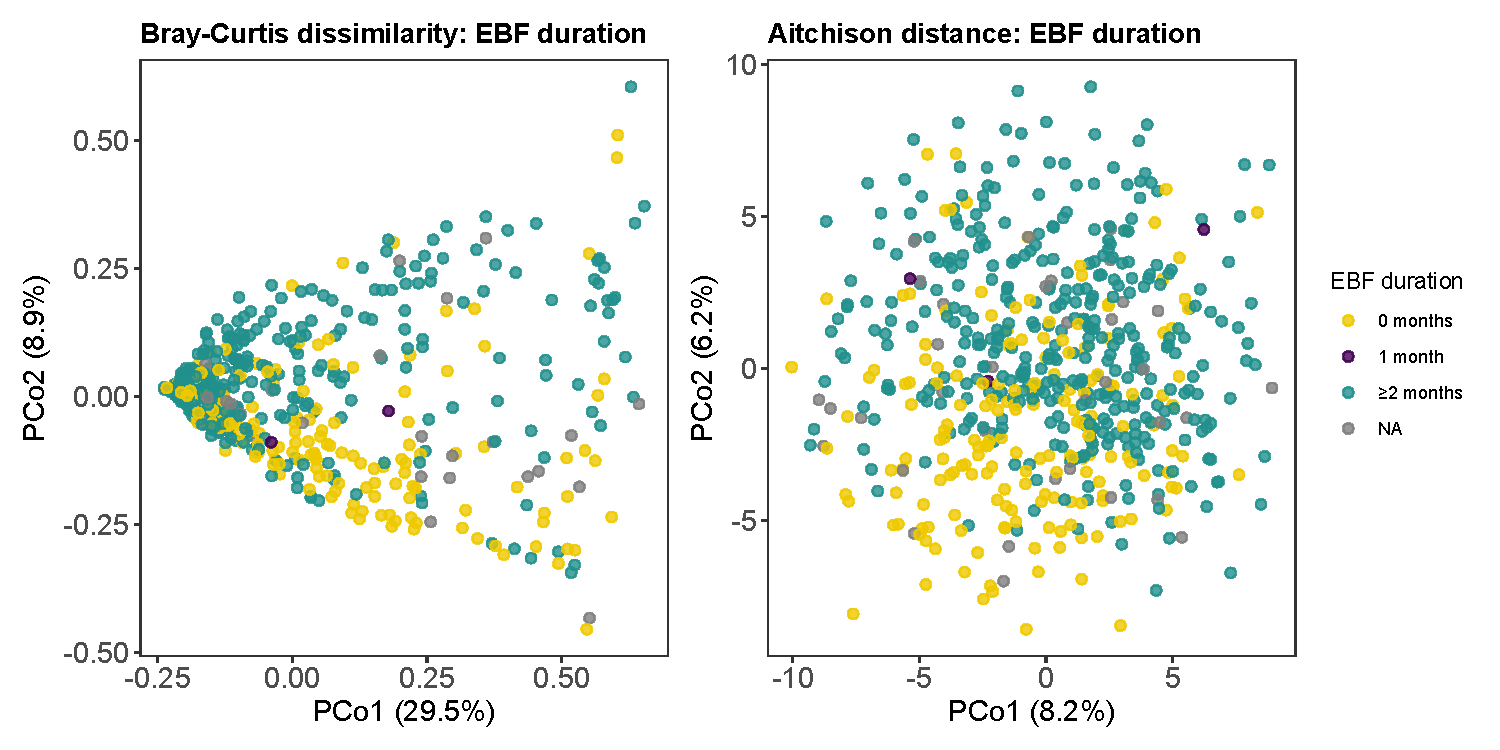
\includegraphics[width=\textwidth]{../ch07_application/figures/04_beta_diversity/thesis_PCoA_colored-5.pdf}
\caption{\textbf{Principal coordinate analysis by EBF duration.} Principal coordinate analysis of between-sample dissimilarities colored by EBF duration. The left panel shows Bray--Curtis dissimilarity computed from relative abundance profiles. The right panel shows Aitchison distance, computed as Euclidean distance after multiplicative replacement of zero counts followed by CLR transformation. Each point represents one stool sample, and the axis labels indicate the proportion of variation represented by the respective coordinate.}
\label{fig:7app:beta_diss:pcoa-exclusive-bf}
\end{figure}

%====================================
\subsection{PERMANOVA}
\label{sec:7app:beta:permanova}
%====================================

To formally assess whether cohort variables explain variation in the between-sample dissimilarity matrices, PERMANOVA was applied to both distance representations, following the distance-based testing framework described in Section~\ref{sec:3community:between:permanova}. The analysis was implemented using the \texttt{adonis2()} function from the \texttt{vegan} package \citep{oksanen2024vegan}. For each cohort variable and distance measure, a separate PERMANOVA model was fitted, and the observed pseudo-$F$ statistic was compared with a permutation distribution obtained from $999$ random permutations of the group labels. For EBF duration, the binary contrast defined in Section~\ref{sec:7app:default_data} was used. Samples with missing values for the respective cohort variable were excluded.

The resulting empirical $p$-values were subsequently refined using \texttt{permApprox}. The refinement used the default configuration described in Section~\ref{sec:6perm:workflow:default_config}, with three analysis-specific settings: a right-sided alternative was used because large pseudo-$F$ statistics indicate stronger evidence against the null hypothesis, the permutation distribution was centered around its median by setting \texttt{null\_center = ``median''}, and multiple testing adjustment was disabled. The reported values therefore correspond to nominal empirical and \texttt{permApprox}-refined $p$-values for each prespecified variable--distance combination. They are interpreted as variable-wise tests of association between each cohort variable and the respective dissimilarity matrix, rather than as a multiplicity-controlled family of simultaneous discoveries across all variables and distance measures.

Table~\ref{tab:7app:beta:permanova} summarizes the PERMANOVA results. For Bray--Curtis dissimilarity, all cohort variables except Sex show significant associations with community composition based on the refined $p$-values. The strongest evidence is observed for BF duration and EBF duration, followed by Country, Smoking, C-section, and Siblings. For Aitchison distance, all inspected cohort variables are significant at the $5\%$ level after $p$-value refinement, including Sex. The smallest refined $p$-values are again obtained for BF duration and EBF duration, indicating that breastfeeding-related variables explain the clearest variation in community composition among the variables considered.

\begin{table}[!htb]
\centering
\caption{\label{tab:7app:beta:permanova}\textbf{PERMANOVA results for between-sample dissimilarities.} PERMANOVA was applied separately to Bray--Curtis dissimilarity and Aitchison distance for all cohort variables. $n$ denotes the number of samples included in the respective test. Samples with missing values for the corresponding cohort variable were excluded, and for EBF duration the binary contrast defined in Section~\ref{sec:7app:default_data} was used. $F$ is the observed pseudo-$F$ statistic obtained with \texttt{adonis2}. \# exceed. denotes the number of permuted statistics greater than or equal to the observed statistic. $p$ (emp.) is the empirical permutation $p$-value based on $999$ permutations, and $p$ (GPD-refined) is the \texttt{permApprox}-refined $p$-value obtained from GPD tail approximation.}
\begin{threeparttable}
\begin{tabular}[t]{l@{\hspace*{1.5em}}rrr@{\hspace*{2em}}l@{\hspace*{2em}}l}
\toprule
Measure & $n$ & $F$ & \# exceed. & $p$ (emp.) & $p$ (GPD-refined)\\
\midrule
\addlinespace[0.3em]
\multicolumn{6}{l}{\textbf{Country}}\\
\hspace{1em}Bray--Curtis & 592 & 4.54 & 0 & 1.00e-03$^{**}$ & 1.18e-04$^{***}$\\
\hspace{1em}Aitchison & 592 & 2.58 & 0 & 1.00e-03$^{**}$ & 9.72e-14$^{***}$\\
\addlinespace[0.3em]
\multicolumn{6}{l}{\textbf{Sex}}\\
\hspace{1em}Bray--Curtis & 592 & 1.36 & 183 & 1.84e-01 & 1.84e-01\\
\hspace{1em}Aitchison & 592 & 1.45 & 33 & 3.40e-02$^{*}$ & 3.51e-02$^{*}$\\
\addlinespace[0.3em]
\multicolumn{6}{l}{\textbf{C-section}}\\
\hspace{1em}Bray--Curtis & 589 & 3.69 & 10 & 1.10e-02$^{*}$ & 7.56e-03$^{**}$\\
\hspace{1em}Aitchison & 589 & 2.48 & 0 & 1.00e-03$^{**}$ & 4.79e-07$^{***}$\\
\addlinespace[0.3em]
\multicolumn{6}{l}{\textbf{BF duration}}\\
\hspace{1em}Bray--Curtis & 580 & 14.30 & 0 & 1.00e-03$^{**}$ & 3.00e-11$^{***}$\\
\hspace{1em}Aitchison & 580 & 6.36 & 0 & 1.00e-03$^{**}$ & 3.91e-97$^{***}$\\
\addlinespace[0.3em]
\multicolumn{6}{l}{\textbf{EBF duration}}\\
\hspace{1em}Bray-Curtis & 554 & 19.58 & 0 & 1.00e-03$^{**}$ & 1.82e-08$^{***}$\\
\hspace{1em}Aitchison & 554 & 10.18 & 0 & 1.00e-03$^{**}$ & 1.18e-13$^{***}$\\
\addlinespace[0.3em]
\multicolumn{6}{l}{\textbf{Smoking}}\\
\hspace{1em}Bray--Curtis & 592 & 5.70 & 1 & 2.00e-03$^{**}$ & 6.81e-04$^{***}$\\
\hspace{1em}Aitchison & 592 & 3.09 & 0 & 1.00e-03$^{**}$ & 5.28e-10$^{***}$\\
\addlinespace[0.3em]
\multicolumn{6}{l}{\textbf{Siblings}}\\
\hspace{1em}Bray--Curtis & 503 & 2.23 & 20 & 2.10e-02$^{*}$ & 1.99e-02$^{*}$\\
\hspace{1em}Aitchison & 503 & 1.58 & 5 & 6.00e-03$^{**}$ & 1.80e-03$^{**}$\\
\bottomrule
\end{tabular}
\begin{tablenotes}
\item $^{***}:p<0.001$; $^{**}:p<0.01$; $^{*}:p<0.05$; $^{.}:p<0.1$.
\end{tablenotes}
\end{threeparttable}
\end{table}

The empirical permutation $p$-values illustrate the finite resolution of the permutation procedure. Whenever no permuted pseudo-$F$ statistic exceeds the observed value, the empirical $p$-value equals $1/(999+1)=0.001$. This occurs for several variables and for both distance measures. The \texttt{permApprox} refinement resolves this discreteness by modeling the upper tail of the corresponding permutation distribution. As a result, variables with the same empirical $p$-value can receive substantially different refined $p$-values, depending not only on the position of the observed statistic relative to the permutation distribution, but also on the shape and variability of that distribution.

This behavior is particularly visible for BF duration and EBF duration. For both variables, the observed pseudo-$F$ statistics are smaller for Aitchison distance than for Bray--Curtis dissimilarity, yet the \texttt{permApprox}-refined $p$-values are much smaller for Aitchison distance. This difference can be understood from the corresponding permutation distributions shown in Figure~\ref{fig:7app:beta_diss:permanova-permutation-distributions}. For the breastfeeding-related variables, the Aitchison permutation distributions are more concentrated, so that the observed statistics lie further in the extreme tail of their respective null distributions despite being numerically smaller than the Bray--Curtis pseudo-$F$ statistics. The refined $p$-values therefore reflect the extremeness of each observed statistic relative to its own distance-specific permutation distribution. The figure additionally includes C-section as a further early-life exposure related to birth mode. The corresponding permutation distributions for the remaining cohort variables are available in the \href{https://github.com/stefpeschel/phd_thesis/tree/main/ch07_application}{\texttt{ch07\_application}} folder of the thesis repository described at the beginning of this chapter.

\begin{figure}[!htb]
\centering
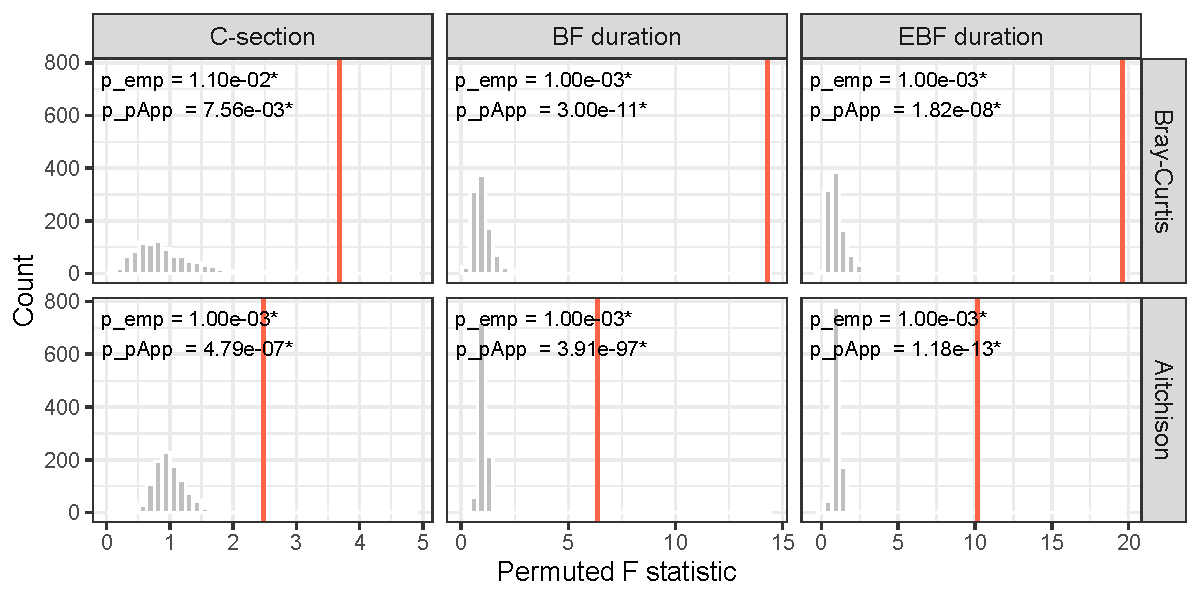
\includegraphics[width=\textwidth]{../ch07_application/figures/04_beta_diversity/thesis_permanova_permapprox_perm_dist_sel-1.pdf}
\caption{\textbf{PERMANOVA permutation distributions with $p$-value refinement.} Histograms show the permutation distributions of the PERMANOVA pseudo-$F$ statistic for each distance measure and three selected cohort variables: BF duration, EBF duration, and C-section. Red vertical lines indicate the observed pseudo-$F$ statistics. The displayed $p$-values correspond to the empirical permutation $p$-value and the \texttt{permApprox}-refined $p$-value. The breastfeeding-related variables illustrate that refined $p$-values depend on the position of the observed statistic relative to the full permutation distribution, and not only on the magnitude of the observed pseudo-$F$ statistic.}
\label{fig:7app:beta_diss:permanova-permutation-distributions}
\end{figure}

Taken together, the PERMANOVA results indicate that several cohort variables are associated with differences in overall community composition. The most consistent and strongest associations are observed for BF duration and EBF duration across both distance measures. Since PERMANOVA can also be sensitive to differences in within-group dispersion, the corresponding dispersion structure is examined in the following subsection using PERMDISP.

%====================================
\subsection{PERMDISP}
\label{sec:7app:beta:permdisp}
%====================================

PERMDISP was applied as described in Section~\ref{sec:3community:between:dispersion} to assess whether cohort variables were associated with differences in within-group dispersion. The same sample exclusions as in the PERMANOVA analysis were used. For EBF duration, this corresponds to the binary contrast defined in Section~\ref{sec:7app:default_data}. For each cohort variable and distance measure, distances of samples to their group centroid were computed and compared between groups. The analysis was implemented using the \texttt{betadisper()} and \texttt{permutest()} functions from the \texttt{vegan} package \citep{oksanen2024vegan}. Empirical $p$-values were computed using $999$ permutations and refined with \texttt{permApprox} using the same configuration as in the PERMANOVA analysis.

Table~\ref{tab:7app:beta:permdisp} summarizes the PERMDISP results. For Bray--Curtis dissimilarity, significant dispersion differences were observed for all variables except Sex. For Aitchison distance, dispersion differences were most pronounced for Country, BF duration, EBF duration, and Smoking, whereas C-section and Siblings showed weaker evidence and Sex showed no indication of dispersion differences. The strongest dispersion effects were again observed for the breastfeeding-related variables, particularly for Aitchison distance. These results indicate that the group differences detected by PERMANOVA should not be interpreted purely as shifts in multivariate location, because for several variables they are accompanied by differences in within-group dispersion.

\begin{table}[!htb]
\centering
\caption{\label{tab:7app:beta:permdisp}\textbf{PERMDISP results for between-sample dissimilarities.} PERMDISP was applied separately to Bray--Curtis dissimilarity and Aitchison distance for all cohort variables. $n$ denotes the number of samples included in the respective test. Samples with missing values for the corresponding cohort variable were excluded, and for EBF duration the binary contrast defined in Section~\ref{sec:7app:default_data} was used. $F$ is the observed test statistic for differences in distances to the group centroid. \# exceed. denotes the number of permuted statistics greater than or equal to the observed statistic. $p$ (emp.) is the empirical permutation $p$-value based on $999$ permutations, and $p$ (GPD-refined) is the \texttt{permApprox}-refined $p$-value obtained from GPD tail approximation.}
\begin{threeparttable}
\begin{tabular}[t]{l@{\hspace*{1.5em}}rrr@{\hspace*{2em}}l@{\hspace*{2em}}l}
\toprule
Measure & $n$ & $F$ & \# exceed. & $p$ (emp.) & $p$ (GPD-refined)\\
\midrule
\addlinespace[0.3em]
\multicolumn{6}{l}{\textbf{Country}}\\
\hspace{1em}Bray--Curtis & 592 & 10.60 & 4 & 5.00e-03$^{**}$ & 2.89e-03$^{**}$\\
\hspace{1em}Aitchison & 592 & 13.30 & 0 & 1.00e-03$^{**}$ & 2.22e-10$^{***}$\\
\addlinespace[0.3em]
\multicolumn{6}{l}{\textbf{Sex}}\\
\hspace{1em}Bray--Curtis & 592 & 2.67 & 215 & 2.16e-01 & 2.16e-01\\
\hspace{1em}Aitchison & 592 & 0.61 & 433 & 4.34e-01 & 4.34e-01\\
\addlinespace[0.3em]
\multicolumn{6}{l}{\textbf{C-section}}\\
\hspace{1em}Bray--Curtis & 589 & 8.87 & 34 & 3.50e-02$^{*}$ & 2.85e-02$^{*}$\\
\hspace{1em}Aitchison & 589 & 3.54 & 66 & 6.70e-02$^{.}$ & 6.93e-02$^{.}$\\
\addlinespace[0.3em]
\multicolumn{6}{l}{\textbf{BF duration}}\\
\hspace{1em}Bray--Curtis & 580 & 14.90 & 1 & 2.00e-03$^{**}$ & 5.88e-04$^{***}$\\
\hspace{1em}Aitchison & 580 & 32.10 & 0 & 1.00e-03$^{**}$ & 2.14e-26$^{***}$\\
\addlinespace[0.3em]
\multicolumn{6}{l}{\textbf{EBF duration}}\\
\hspace{1em}Bray-Curtis & 554 & 16.00 & 4 & 5.00e-03$^{**}$ & 4.21e-03$^{**}$\\
\hspace{1em}Aitchison & 554 & 61.04 & 0 & 1.00e-03$^{**}$ & 2.78e-14$^{***}$\\
\addlinespace[0.3em]
\multicolumn{6}{l}{\textbf{Smoking}}\\
\hspace{1em}Bray--Curtis & 592 & 6.74 & 47 & 4.80e-02$^{*}$ & 4.63e-02$^{*}$\\
\hspace{1em}Aitchison & 592 & 15.70 & 0 & 1.00e-03$^{**}$ & 2.63e-04$^{***}$\\
\addlinespace[0.3em]
\multicolumn{6}{l}{\textbf{Siblings}}\\
\hspace{1em}Bray--Curtis & 503 & 5.88 & 42 & 4.30e-02$^{*}$ & 4.77e-02$^{*}$\\
\hspace{1em}Aitchison & 503 & 2.63 & 83 & 8.40e-02$^{.}$ & 8.03e-02$^{.}$\\
\bottomrule
\end{tabular}
\begin{tablenotes}
\item $^{***}:p<0.001$; $^{**}:p<0.01$; $^{*}:p<0.05$; $^{.}:p<0.1$.
\end{tablenotes}
\end{threeparttable}
\end{table}


Figure~\ref{fig:7app:beta:centroid-distances} visualizes the PERMDISP results for the same three selected variables as above: BF duration, EBF duration, and C-section. The corresponding plots for the remaining cohort variables are available in the \href{https://github.com/stefpeschel/phd_thesis/tree/main/ch07_application}{\texttt{ch07\_application}} folder of the thesis repository described at the beginning of this chapter. For BF duration and EBF duration, the boxplots indicate clear differences in the heterogeneity of samples around their respective group centroids. This is especially visible for Aitchison distance, where groups with shorter or no breastfeeding tend to show larger distances to the centroid than the longer breastfeeding groups. C-section shows a weaker but still visible difference in dispersion, particularly for Bray--Curtis dissimilarity. These results indicate that the corresponding PERMANOVA findings should be interpreted as differences in overall group structure, while acknowledging that part of the signal may be attributable to differences in within-group dispersion rather than only to shifts in group centroids.

\begin{figure}[!htb]
\centering
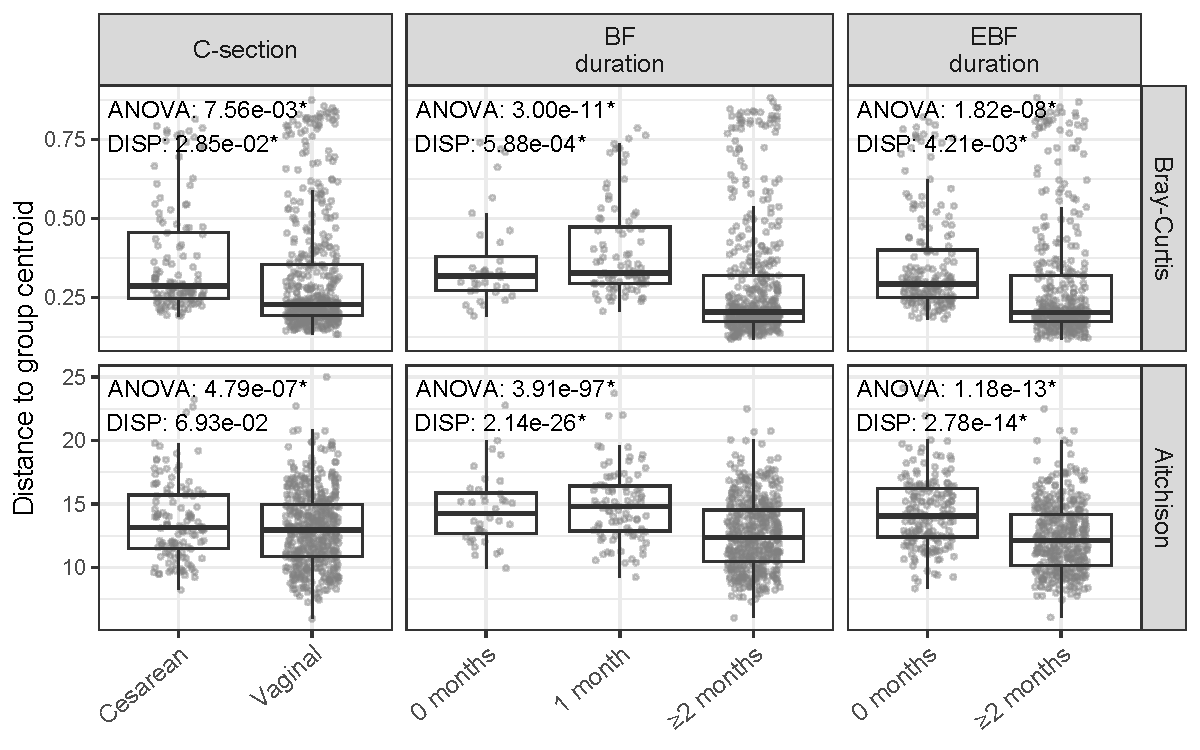
\includegraphics[width=\textwidth]{../ch07_application/figures/04_beta_diversity/thesis_beta_centroid_dist_sel-1.pdf}
\caption{\label{fig:7app:beta:centroid-distances}\textbf{Distances to group centroids for selected cohort variables.} Boxplots show the distances of samples to their respective group centroid for BF duration, EBF duration, and C-section. The upper row shows Bray--Curtis dissimilarity, and the lower row shows Aitchison distance. Points represent individual samples. The annotations report the \texttt{permApprox}-refined $p$-values from PERMANOVA and PERMDISP.}
\end{figure}

Overall, the PERMDISP analysis shows that dispersion differences are present for several cohort variables and are particularly pronounced for the breastfeeding-related variables. Thus, the corresponding PERMANOVA results should not be interpreted solely as evidence for shifts in group centroids. Instead, they indicate differences in the overall structure of the microbial community profiles, which may reflect both changes in average composition and differences in within-group heterogeneity. This observation is relevant for the subsequent analyses, because BF duration and EBF duration remain the variables with the most consistent community-level signal, but their effects appear to involve both location and dispersion components.

%%%%%%%%%%%%%%%%%%%%%%%%%%%%%%%%%%%%%
\section{Regression models for compositional responses}
\label{sec:7app:regression}
%%%%%%%%%%%%%%%%%%%%%%%%%%%%%%%%%%%%%

As a model-based complement to the distance-based analyses, CLR-based multivariate regression was applied to the genus-level microbiome profiles. The analysis followed the framework described in Section~\ref{sec:3community:regression} and used the default CLR representation defined in Section~\ref{sec:7app:default_data}. Whereas PERMANOVA assessed each cohort variable in a separate one-variable model, the regression approach allowed all covariates to be included jointly and each covariate to be tested conditionally on the others.

The regression model included the same cohort variables as the preceding community-level analyses, namely Country, Sex, C-section, BF duration, EBF duration, Smoking, and Siblings, as summarized in Table~\ref{tab:7app:sample_characteristics}. To ensure that all full-versus-reduced model comparisons were based on the same samples, a complete-case data set was constructed across all model covariates. In addition, the binary EBF contrast defined in Section~\ref{sec:7app:default_data} was used, so that the three samples with EBF duration of 1 month were excluded. The final regression analysis was therefore based on $n=484$ samples and $p=117$ genus-level taxa.

The fitted full model yields one coefficient for each model term and each CLR coordinate. Figure~\ref{fig:7app:regression:coefficient-heatmap} shows a reduced coefficient heatmap for the $20$ genera with the largest maximum absolute coefficient across all model terms. The heatmap is descriptive and is not used for taxon-level inference. It nevertheless provides a compact overview of the multivariate effect pattern and shows that the strongest fitted coefficients are not concentrated in a single covariate, but occur across several early-life variables. For categorical covariates, rows correspond to contrasts relative to the respective reference category. Positive coefficients indicate larger CLR values for the corresponding genus-level taxon relative to the sample-wise geometric mean, whereas negative coefficients indicate smaller CLR values on the same scale. The complete heatmap including all genus-level taxa is available in the \href{https://github.com/stefpeschel/phd_thesis/tree/main/ch07_application}{\texttt{ch07\_application}} folder of the thesis repository described at the beginning of this chapter.

\begin{figure}[!htb]
\centering
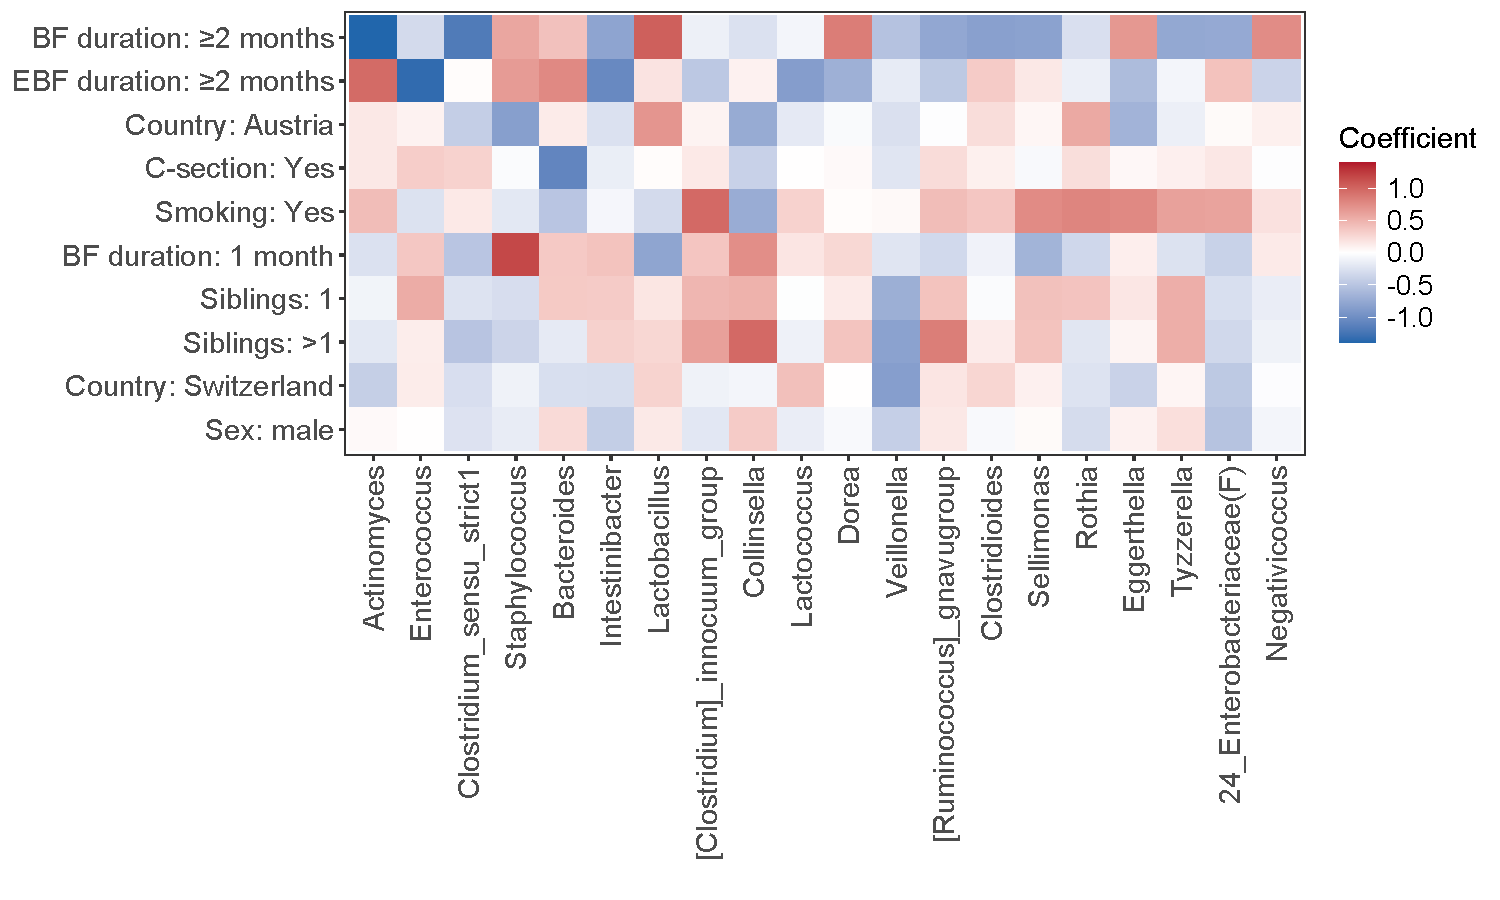
\includegraphics[width=\textwidth]{../ch07_application/figures/05_regression/thesis_coefficient_heatmap_top20-1.pdf}
\caption{\label{fig:7app:regression:coefficient-heatmap}\textbf{Reduced coefficient heatmap for CLR-based multivariate regression.} The heatmap shows fitted regression coefficients for the $20$ genus-level taxa with the largest maximum absolute coefficient across all model terms. Rows correspond to model terms, and columns correspond to genus-level taxa. For categorical covariates, coefficients represent contrasts relative to the reference category. Red values indicate positive coefficients on the CLR scale, whereas blue values indicate negative coefficients. The heatmap is descriptive and is not used for taxon-level inference.}
\end{figure}

For inference, each covariate was tested by comparing the full model with a reduced model in which the respective covariate was omitted, as described in Section~\ref{sec:3community:regression:testing}. The test statistic $t_j$ was defined as the reduction in multivariate residual sum of squares when covariate $j$ was included in the model. Larger values therefore indicate that the covariate explains more variation in the CLR-transformed microbial profile, conditional on the other covariates in the model. For each covariate, an empirical permutation $p$-value was computed from $999$ random permutations of the corresponding covariate. The resulting $p$-values were refined using \texttt{permApprox} with the same configuration as in the PERMANOVA analysis, namely a right-sided test, median centering of the permutation distribution, and no multiple testing adjustment. The reported $p$-values are therefore interpreted as nominal variable-wise $p$-values for the prespecified covariates.


The regression-based global tests in Table~\ref{tab:7app:regression:global-tests} identify EBF duration, Country, and BF duration as the strongest covariates, with no permuted statistic exceeding the observed statistic in $999$ permutations. The GPD refinement separates these three empirical $p$-values, which are all equal to $0.001$ before refinement. The smallest refined $p$-value is obtained for EBF duration, followed by Country and BF duration. Smoking also shows evidence of an association with the CLR-transformed microbial composition, whereas Siblings shows weaker evidence and Sex and C-section show no clear association after conditioning on the other covariates in the joint model.

\begin{table}[H]
\centering
\caption{\textbf{Permutation-based global tests in multivariate regression.} The table summarizes global covariate tests from the CLR-based multivariate regression model. All tests were performed on the same complete-case data set with $n=484$ samples and $117$ genus-level taxa. The statistic $t_j$ is the reduction in multivariate residual sum of squares when the covariate is added to the model. \# exceed. denotes the number of permuted statistics greater than or equal to the observed statistic. $p$ (emp.) is the empirical permutation $p$-value based on $999$ permutations, and $p$ (GPD-refined) is the \texttt{permApprox}-refined $p$-value obtained from GPD tail approximation.}
\label{tab:7app:regression:global-tests}
\centering
\begin{threeparttable}
\begin{tabular}[t]{lrrll}
\toprule
Variable & $t_j$ & \# exceed & $p$ (emp.) & $p$ (GPD-refined)\\
\midrule
Country & 699.03 & 0 & 1.00e-03$^{**}$ & 3.51e-06$^{***}$\\
Sex & 225.51 & 107 & 1.08e-01 & 1.08e-01\\
C-section & 217.65 & 147 & 1.48e-01 & 1.48e-01\\
BF duration & 641.49 & 0 & 1.00e-03$^{**}$ & 4.14e-05$^{***}$\\
EBF duration & 450.95 & 0 & 1.00e-03$^{**}$ & 8.78e-07$^{***}$\\
Smoking & 274.78 & 29 & 3.00e-02$^{*}$ & 2.41e-02$^{*}$\\
Siblings & 436.92 & 77 & 7.80e-02$^{.}$ & 7.22e-02$^{.}$\\
\bottomrule
\end{tabular}
\begin{tablenotes}
\item $^{***}:p<0.001$; $^{**}:p<0.01$; $^{*}:p<0.05$; $^{.}:p<0.1$.
\end{tablenotes}
\end{threeparttable}
\end{table}

These results partly agree with the distance-based PERMANOVA analysis, in which breastfeeding-related variables also showed the most consistent community-level associations. At the same time, the regression model has a different interpretation: each covariate is tested conditionally on the remaining covariates in the model, whereas the preceding PERMANOVA analyses considered separate one-variable models. The weaker regression signal for C-section therefore does not contradict the PERMANOVA result, but suggests that its contribution is less pronounced after accounting for the other early-life variables included in the multivariate model. Overall, the compositional-response regression supports the relevance of breastfeeding-related variables while providing a complementary model-based view of community-level covariate effects.

%%%%%%%%%%%%%%%%%%%%%%%%%%%%%%%%%%%%%
\section{Compositional equivalence}
\label{sec:7app:compositional-equivalence}
%%%%%%%%%%%%%%%%%%%%%%%%%%%%%%%%%%%%%

As a final community-level comparison, compositional equivalence was applied to selected two-group contrasts. In contrast to PERMANOVA, which operates on pairwise sample dissimilarities, compositional equivalence compares group mean composition in CLR space and summarizes the largest standardized coordinate-wise mean difference by a single global statistic, as described in Section~\ref{sec:3community:compositional_equivalence}. The analysis used the default CLR representation defined in Section~\ref{sec:7app:default_data}.

Because compositional equivalence is formulated as a two-group comparison, the analysis was restricted to selected binary or binarized contrasts. C-section, Sex, and Smoking were already binary variables. For BF duration and EBF duration, the main contrast compared samples with no breastfeeding to samples with breastfeeding duration $\ge 2$ months, omitting the sparse 1-month category as described in Section~\ref{sec:7app:default_data}. For Siblings, the variable was collapsed into children without siblings and children with at least one sibling. Country was omitted because this analysis focused on biologically interpretable two-group contrasts, whereas Country is a three-level cohort variable that may capture geographic, cohort-specific, and technical differences. The resulting contrast definitions are summarized in Table~\ref{tab:7app:comp-equivalence:contrasts}.

\begin{table}[H]
\centering
\caption{\textbf{Definition of selected two-group contrasts for compositional equivalence.} Group 1 and group 2 define the direction of the signed standardized CLR mean differences shown in Figure~\ref{fig:7app:comp-equivalence:top10-ebf}. Samples with missing values for the corresponding variable were excluded; for BF duration and EBF duration, the sparse 1-month category was additionally omitted.}
\label{tab:7app:comp-equivalence:contrasts}
\begin{tabular}[t]{llrlr}
\toprule
Contrast     & Group 1  & $n_1$ & Group 2 & $n_2$\\
\midrule
C-section    & Cesarean & 121 & Vaginal & 468\\
BF duration  & 0 months & 36 & $\ge 2$ months & 456\\
EBF duration & 0 months & 179 & $\ge 2$ months & 375\\
Sex          & Female   & 294 & Male & 298\\
Smoking      & No       & 529 & Yes & 63\\
Siblings     & 0        & 46 & $\ge 1$ & 457\\
\bottomrule
\end{tabular}
\end{table}

For each contrast, group differences were first evaluated coordinate-wise on the CLR scale. The resulting coordinate-wise contributions $m_i$, defined in Equation~\ref{eq:3community:comp_equivalence:coordinate_contribution}, form the building blocks of the global compositional equivalence statistic. They are therefore useful for describing which taxa contribute most to the maximum statistic, but are not interpreted as separate taxon-level hypothesis tests. Since $m_i$ is based on a squared mean difference, it does not contain information about the direction of the contrast. For visualization, the direction was therefore added through the signed standardized CLR mean difference $(\bar{y}_i^{(1)}-\bar{y}_i^{(2)})/\sqrt{\hat{\gamma}_{ii}}$, where positive values indicate larger CLR means in group 1 and negative values indicate larger CLR means in group 2. Since EBF duration was selected as the main grouping variable for subsequent comparative analyses, Figure~\ref{fig:7app:comp-equivalence:top10-ebf} shows the ten genera with the largest coordinate-wise contributions for this contrast. The corresponding plots for the remaining contrasts are available in the \href{https://github.com/stefpeschel/phd_thesis/tree/main/ch07_application}{\texttt{ch07\_application}} folder of the thesis repository described at the beginning of this chapter.

\begin{figure}[!htb]
\centering
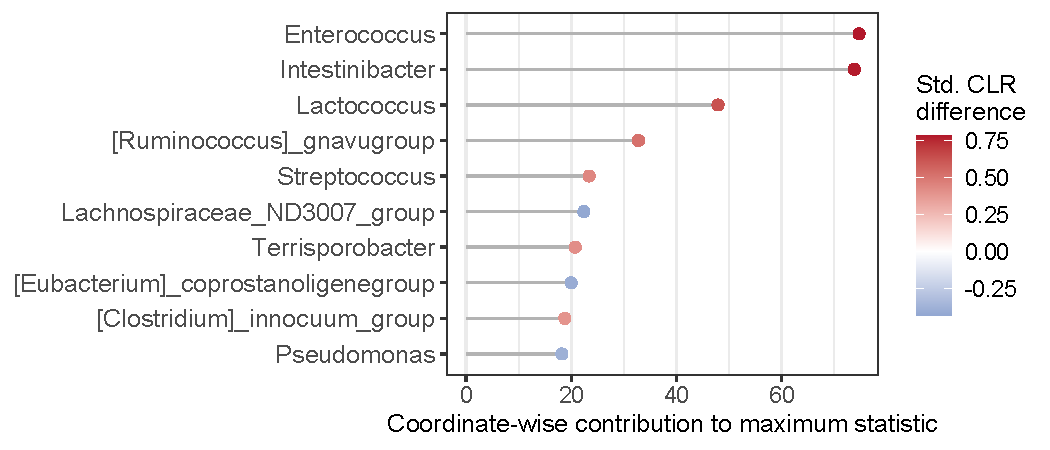
\includegraphics[width=0.85\textwidth]{../ch07_application/figures/06_comp_equivalence/thesis_taxon_contrast_top10_selected-1.pdf}
\caption{\label{fig:7app:comp-equivalence:top10-ebf}\textbf{Top coordinate-wise contributions for EBF duration.} The plot shows the ten genera with the largest coordinate-wise contributions $m_i$ from Equation~\ref{eq:3community:comp_equivalence:coordinate_contribution} for the contrast between no EBF and EBF duration $\ge 2$ months. Points show the squared, sample-size-weighted contribution to the maximum statistic. Colors indicate the signed standardized CLR mean difference and therefore encode the direction of the contrast. Positive values correspond to larger CLR means in group 1, as defined in Table~\ref{tab:7app:comp-equivalence:contrasts}.}
\end{figure}

For EBF duration, group 1 corresponds to children without EBF and group 2 to children with EBF duration $\ge 2$ months. Thus, positive signed standardized CLR mean differences indicate larger CLR values in the no-EBF group. The largest coordinate-wise contributions are observed for \emph{Enterococcus} and \emph{Intestinibacter}, followed by \emph{Lactococcus} and the \emph{[Ruminococcus] gnavus group}. Most of the largest signed differences are positive, indicating that the strongest coordinate-wise differences are driven by genera with higher relative representation, on the CLR scale, among children without EBF. Although the formal focus of the compositional equivalence test is the community-level maximum statistic, these taxon-wise contributions provide a useful descriptive link to the subsequent feature-level analyses.

The global compositional equivalence statistic $M_n$ was then computed as the maximum over all coordinate-wise contributions, as defined in Equation~\ref{eq:3community:comp_equivalence:maximum_statistic}. \citet{cao2018twosample} show that the centered statistic $M_n - 2\log(p) + \log\log(p)$ can be approximated by a Gumbel distribution under asymptotic assumptions, where $p$ denotes the number of CLR coordinates. These assumptions are not necessarily fulfilled in finite, sparse microbiome data. Indeed, \citet{sommer2022randomizationbased} compare this asymptotic approximation with permutation-based null distributions in their Supplementary Figure~J and show that the Gumbel approximation can differ markedly from the empirical permutation distribution, with corresponding differences in $p$-values. We performed the same comparison for the PASTURE contrasts in Appendix Figure~\ref{fig:app:7app:comp_equivalence_gumbel_comparison}. The corresponding asymptotic Gumbel $p$-values are included alongside the permutation-based $p$-values in Table~\ref{tab:7app:comp-equivalence:pvals}. As in \citep{sommer2022randomizationbased}, the permutation distributions were not uniformly well approximated by the Gumbel distribution, and the asymptotic $p$-values differed from the permutation-based $p$-values for several contrasts.

Therefore, the following inference follows the randomization-based approach of \citet{sommer2022randomizationbased} rather than relying on the asymptotic Gumbel approximation. For each contrast, the observed value of $M_n$ was compared with a permutation distribution obtained from $999$ random permutations of the group labels. Since large values of $M_n$ indicate stronger evidence against equality of mean CLR composition, a right-sided test was used. The resulting empirical $p$-values were refined with \texttt{permApprox} using the same configuration as in the preceding community-level analyses, including median centering of the permutation distribution and no multiple testing adjustment. The reported $p$-values are therefore interpreted as nominal $p$-values for the selected two-group contrasts.

The results in Table~\ref{tab:7app:comp-equivalence:pvals} indicate clear differences in mean CLR composition for C-section, BF duration, and EBF duration. The strongest signal is observed for EBF duration, for which the observed statistic is substantially larger than for the other contrasts and exceeds all permuted statistics. This extremeness cannot be expressed by the empirical permutation $p$-value, which is limited by the number of permutations, but is reflected in the much smaller GPD-refined $p$-value. BF duration and C-section also show significant differences, although their refined $p$-values are considerably less extreme. In contrast, Sex, Smoking, and Siblings show no evidence against equality of mean CLR composition for the selected two-group contrasts.

\begin{table}[H]
\centering
\caption{\textbf{Compositional equivalence results for selected contrasts.} The group definitions and corresponding sample sizes are given in Table~\ref{tab:7app:comp-equivalence:contrasts}. $M_n$ is the maximum standardized squared CLR mean difference. $M_n^c = M_n - 2\log(p) + \log\log(p)$ is the centered statistic used for the asymptotic Gumbel approximation. \# exceed: number of permuted statistics $\geq$ observed. $p$ (emp.): empirical permutation $p$-value ($999$ permutations); $p$ (GPD-ref.): $p$-value refined with \texttt{permApprox}; $p$ (asym.): asymptotic Gumbel $p$-value.}
\label{tab:7app:comp-equivalence:pvals}
\centering
\begin{threeparttable}
\begin{tabular}[t]{lrrrlll}
\toprule
Contrast & $M_n$ & $M_n^c$ & \# exceed & $p$ (emp.) & $p$ (GPD-ref.) & $p$ (asym.)\\
\midrule
C-section & 25.06 & 17.09 & 0 & 1.00e-03$^{**}$ & 5.26e-04$^{***}$ & 1.09e-04$^{***}$\\
BF duration & 33.16 & 25.19 & 3 & 4.00e-03$^{**}$ & 2.99e-03$^{**}$ & 1.91e-06$^{***}$\\
EBF duration & 74.72 & 66.75 & 0 & 1.00e-03$^{**}$ & 2.31e-66$^{***}$ & 1.78e-15$^{***}$\\
Sex & 9.79 & 1.83 & 157 & 1.58e-01 & 1.58e-01 & 2.03e-01\\
Smoking & 13.91 & 5.95 & 119 & 1.20e-01 & 1.20e-01 & 2.84e-02$^{*}$\\
\addlinespace
Siblings & 14.17 & 6.21 & 123 & 1.24e-01 & 1.24e-01 & 2.50e-02$^{*}$\\
\bottomrule
\end{tabular}
\begin{tablenotes}
\item $^{***}:p<0.001$; $^{**}:p<0.01$; $^{*}:p<0.05$; $^{.}:p<0.1$.
\end{tablenotes}
\end{threeparttable}
\end{table}

Overall, compositional equivalence supports the central role of breastfeeding-related variables in the PASTURE application. In particular, EBF duration shows a strong difference in mean CLR composition between children without EBF and children with EBF duration $\ge 2$ months. Together with the PERMANOVA, PERMDISP, and regression results, this motivates using EBF duration as the main grouping variable for the subsequent feature-level and network-based analyses.

%%%%%%%%%%%%%%%%%%%%%%%%%%%%%%%%%%%%%
\section{Exploratory feature-level analysis}
\label{sec:7app:feature-level-exploration}
%%%%%%%%%%%%%%%%%%%%%%%%%%%%%%%%%%%%%

The preceding community-level analyses identified the breastfeeding-related variables as the most consistent variables associated with differences in the infant gut microbiome. Both BF duration and EBF duration showed strong signals across the community-level analyses. In the PERMANOVA and PERMDISP analyses presented in Section~\ref{sec:7app:beta}, the effects were larger for BF duration, whereas EBF duration yielded smaller $p$-values in the regression and compositional equivalence analyses presented in Sections~\ref{sec:7app:regression} and~\ref{sec:7app:compositional-equivalence}. Since a binary grouping based on BF duration would result in more unbalanced group sizes, EBF duration was selected as the main grouping variable for the subsequent feature-level and network-based analyses. The following comparative analyses therefore use the binary EBF contrast defined in Section~\ref{sec:7app:default_data}, comparing children without EBF ($n=179$) with children with EBF duration $\ge 2$ months ($n=375$).

As a first step, exploratory taxon-level summaries were used to characterize the genus-level composition of the default analysis data set and the two EBF groups. Relative abundances were used for descriptive composition summaries, whereas CLR coordinates were used for visualizing transformed taxon profiles. Both representations are defined in Section~\ref{sec:7app:default_data}. The exploratory analyses are descriptive and are not intended to provide formal taxon-level inference.

Figure~\ref{fig:7app:exploration:prevalence-abundance} first gives an overview of the retained genera without considering the EBF grouping. It displays each genus by its prevalence and mean relative abundance in the filtered genus-level data set. Most retained genera have low mean relative abundance and moderate prevalence, whereas a smaller set of dominant genera is both highly prevalent and comparatively abundant. \emph{Bifidobacterium} is located in the upper right region, indicating high prevalence and high mean relative abundance. Other dominant genera, including \emph{Escherichia-Shigella}, \emph{Streptococcus}, \emph{Bacteroides}, \emph{Enterococcus}, and the \emph{[Ruminococcus] gnavus group}, also stand out from the remaining low-abundance genera. This plot provides the feature-level background for the subsequent group-specific summaries.

\begin{figure}[!htb]
\centering
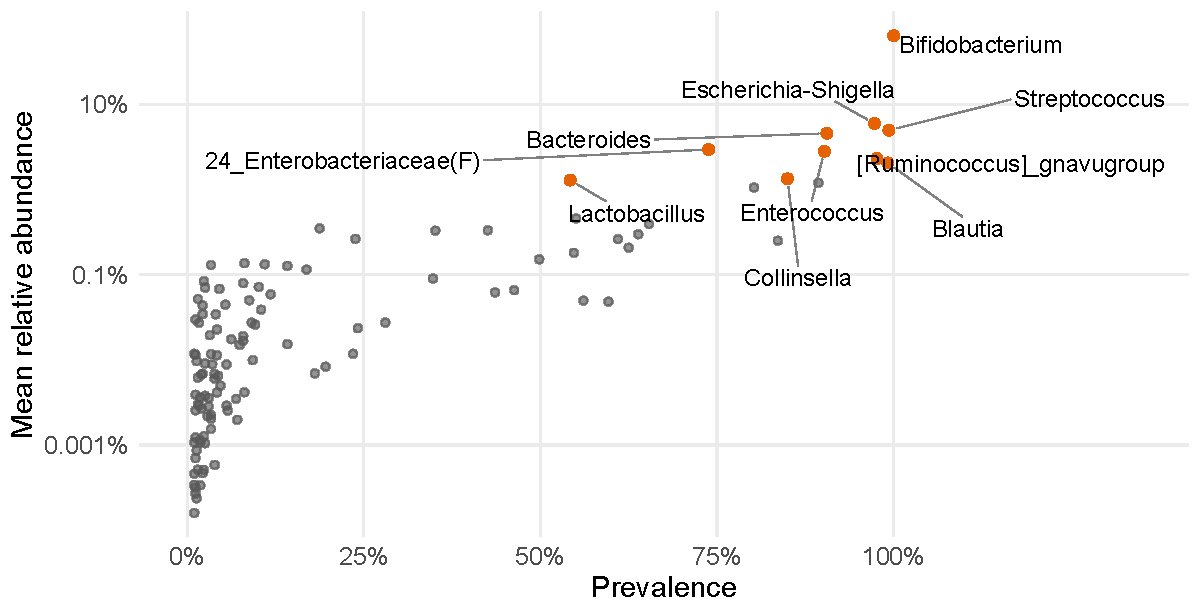
\includegraphics[width=\textwidth]{../ch07_application/figures/07_exploration/thesis_prevalence_abundance-1.pdf}
\caption{\label{fig:7app:exploration:prevalence-abundance}\textbf{Prevalence and mean relative abundance of retained genera.} Each point represents one genus after prevalence filtering. The highlighted and labeled points show the ten genera with the largest mean relative abundances. The y-axis is displayed on a logarithmic scale to show both dominant and low-abundance genera.}
\end{figure}

The following plots focus on the comparison between the two EBF groups. Figure~\ref{fig:7app:exploration:composition-barplot} shows the mean relative abundance of the dominant genera by EBF group. The composition is dominated by \emph{Bifidobacterium} in both groups, reflecting the characteristic dominance of this genus in the early infant gut. The remaining genera contribute smaller proportions, with visible differences between the non-EBF and EBF groups for several taxa, including \emph{Bacteroides}, \emph{Enterococcus}, \emph{Streptococcus}, and \emph{Escherichia-Shigella}. Since this plot is based on relative abundances, the displayed patterns may be affected by compositional effects and should not be interpreted as absolute abundance changes. The CLR coordinates shown in Figure~\ref{fig:7app:exploration:clr-violin} provide a complementary log-ratio view of the same group comparison. The group labeled ``not compared'' is shown for completeness and contains samples not used in the binary EBF comparison.

\begin{figure}[!htb]
\centering
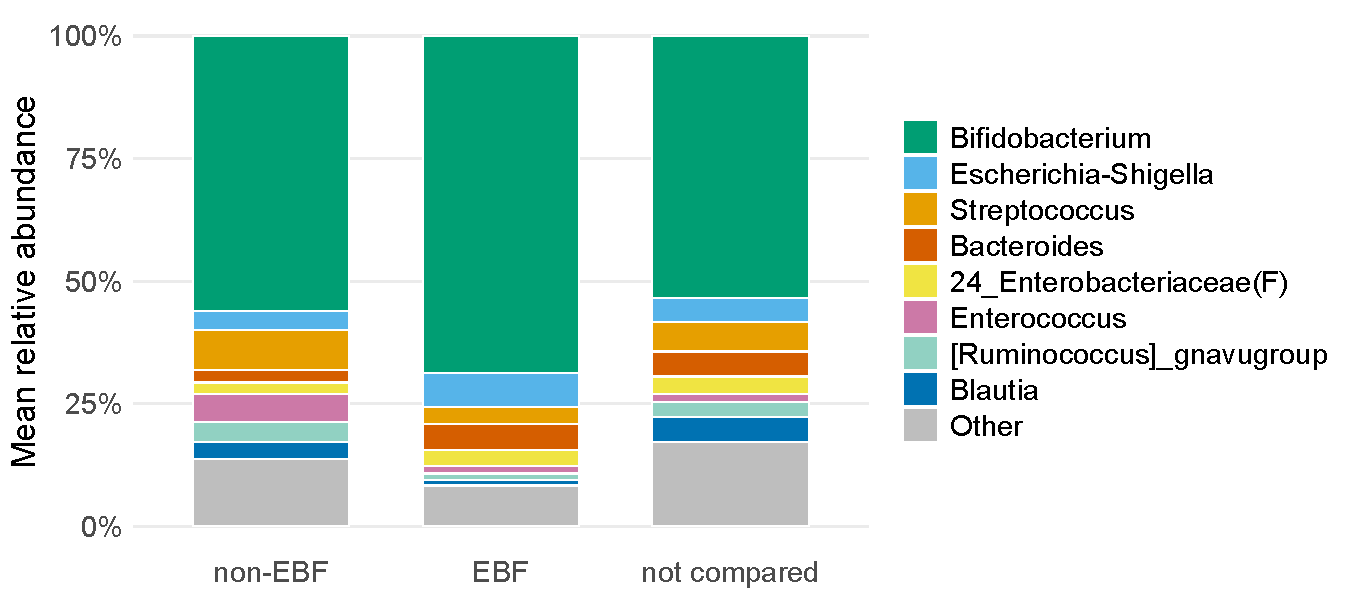
\includegraphics[width=\textwidth]{../ch07_application/figures/07_exploration/thesis_relative_abundance_barplot-1.pdf}
\caption{\label{fig:7app:exploration:composition-barplot}\textbf{Mean genus-level composition by EBF group.} Stacked bars show the mean relative abundances of the dominant genera in the non-EBF group, the EBF group, and samples not included in the EBF comparison. The category ``Other'' summarizes all remaining genera. The plot is descriptive and is based on relative abundances.}
\end{figure}

Figure~\ref{fig:7app:exploration:clr-violin} shows the distributions of CLR coordinates for six dominant genera in the two EBF groups. This representation is closer to the transformed scale used in the following feature-level analyses and avoids interpreting relative-abundance differences as absolute abundance changes. The violin plots indicate differences not only in location but also in distributional shape and variability between the two EBF groups. For example, \emph{Enterococcus} shows higher CLR coordinates in the non-EBF group, whereas \emph{Bacteroides} tends to show higher CLR coordinates in the EBF group. These patterns suggest that feature-level comparisons should not be restricted to mean differences alone. Instead, differential abundance and differential distribution analyses may provide complementary information.

\begin{figure}[!htb]
\centering
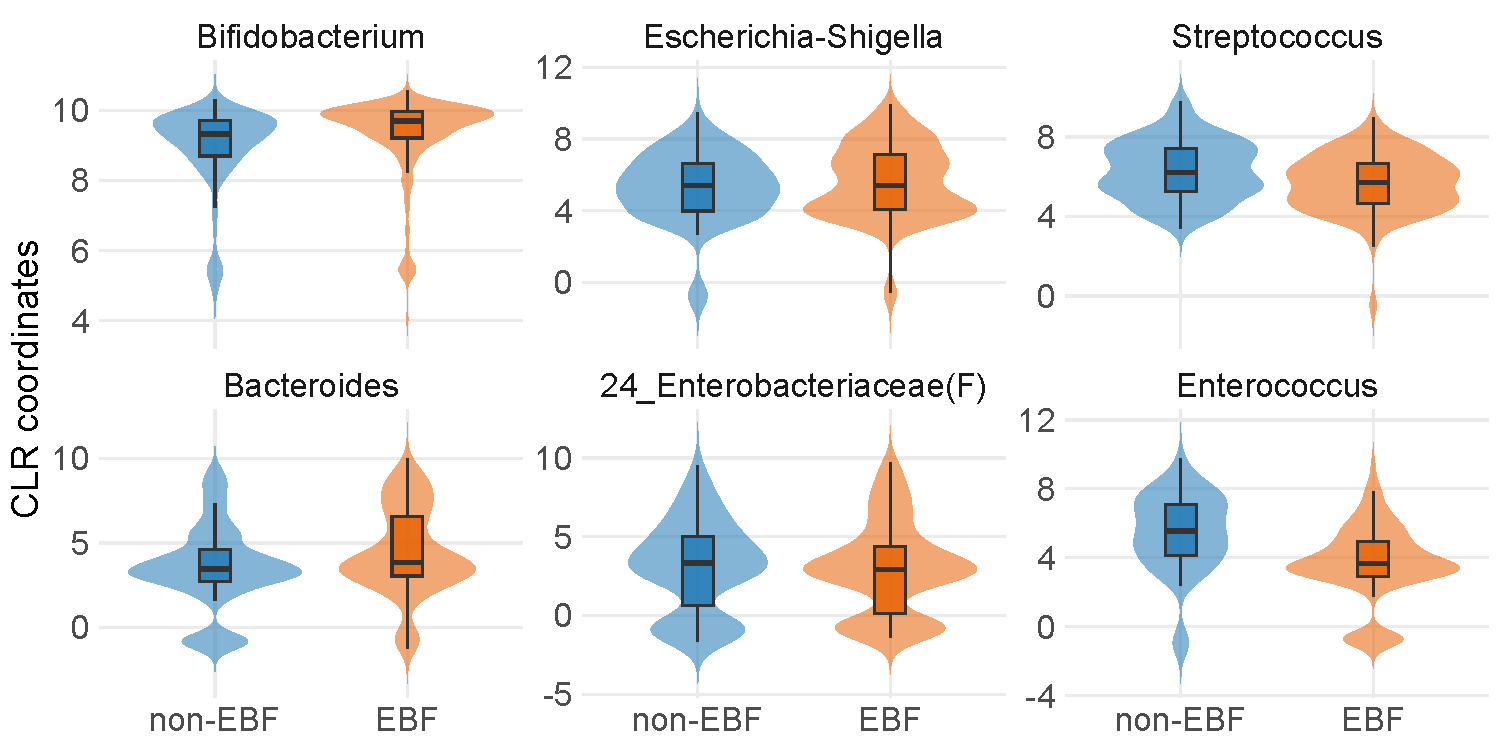
\includegraphics[width=\textwidth]{../ch07_application/figures/07_exploration/thesis_selected_taxon_violin-1.pdf}
\caption{\textbf{CLR coordinates of selected dominant genera by EBF group.} Violin plots and embedded boxplots show the distributions of CLR coordinates for six dominant genera in the non-EBF and EBF groups. Zeros were handled by multiplicative replacement before CLR transformation. The plot is descriptive and does not represent feature-level hypothesis tests.}
\label{fig:7app:exploration:clr-violin}
\end{figure}

Taken together, the exploratory feature-level summaries show visible group differences in the relative-abundance composition and CLR-coordinate distributions of several dominant genera. These observations are consistent with the community-level results but remain descriptive. Formal feature-level comparisons are therefore performed in the following sections using differential abundance and differential distribution analyses.

%%%%%%%%%%%%%%%%%%%%%%%%%%%%%%%%%%%%%
\section{Differential abundance analysis}
\label{sec:7app:differential-abundance}
%%%%%%%%%%%%%%%%%%%%%%%%%%%%%%%%%%%%%

The exploratory feature-level summaries in the previous section suggested visible differences between the two EBF groups for several dominant genera. To formally assess feature-wise abundance differences, differential abundance analysis was performed using DACOMP, as introduced in Section~\ref{sec:4feature:dacomp}. The method is implemented in the R package \texttt{dacomp} \citep{Brill2021dacomp}. The analysis used the binary EBF contrast defined in Section~\ref{sec:7app:default_data}, comparing children without EBF ($n=179$) with children with EBF duration $\ge 2$ months ($n=375$).

%====================================
\subsection{Analysis setup and DACOMP reference set}
\label{sec:7app:differential-abundance:setup}
%====================================

DACOMP was applied to the genus-level count matrix corresponding to the default analysis data set defined in Section~\ref{sec:7app:default_data}, yielding $n=554$ samples and $117$ retained genera. This is a method-specific deviation from the CLR-based representation used in the preceding community-level analyses. DACOMP uses a count-based reference framework: compositionality is addressed by comparing each tested taxon relative to a set of taxa selected to be comparatively stable across samples, while differences in library size are handled through a method-specific subsampling step within the testing procedure. The resulting differential abundance statements are therefore relative to the corresponding reference structure and should not be interpreted as statements about absolute microbial abundances. We used \texttt{dacomp}'s ability to test all retained taxa, including taxa selected for the reference set. When such a reference taxon was itself tested, it was temporarily removed from the reference set for that test.

The reference selection step is summarized in Figure~\ref{fig:7app:da:reference-score}. The diagnostic plot shows the DACOMP reference score against the prevalence of each retained genus. Genera selected as reference taxa are shown in green, while the remaining genera are shown in grey. In total, $91$ of the $117$ retained genera were selected as reference taxa using a minimum total reference abundance criterion of $50$. Most reference taxa have low to moderate prevalence and low DACOMP scores, indicating comparatively stable behavior according to the reference-selection criterion. A few highly prevalent genera, including \emph{Bifidobacterium}, \emph{Blautia}, and \emph{Akkermansia}, were also selected as reference taxa.

\begin{figure}[!htb]
\centering
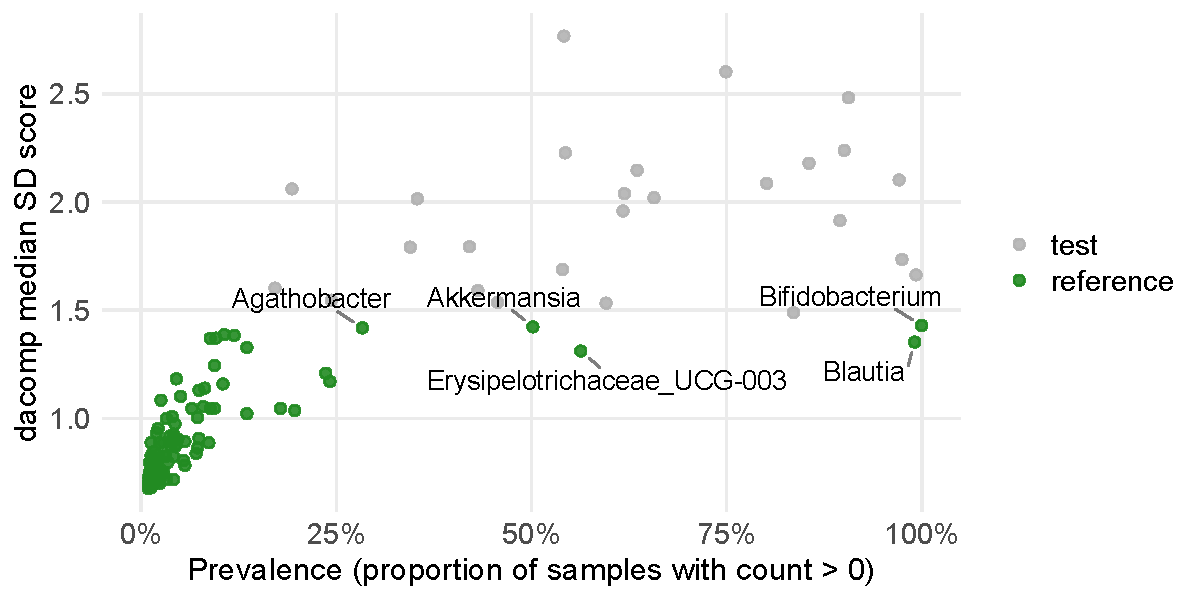
\includegraphics[width=0.9\textwidth]{../ch07_application/figures/08_diff_abundance/thesis_dacomp_reference_score_plot-1.pdf}
\caption{\label{fig:7app:da:reference-score}\textbf{DACOMP reference-score diagnostic.} Each point represents one retained genus. The x-axis shows the prevalence, defined as the proportion of samples with a positive count, and the y-axis shows the DACOMP median standard-deviation score used for reference selection. Green points indicate genera selected for the reference set, and grey points indicate genera not selected as reference taxa. Labeled genera are selected reference taxa with prevalence of at least $25\%$.}
\end{figure}

%====================================
\subsection{Permutation resolution and p-value refinement}
\label{sec:7app:differential-abundance:pvalue-refinement}
%====================================

\begin{figure}[H]
	\centering
	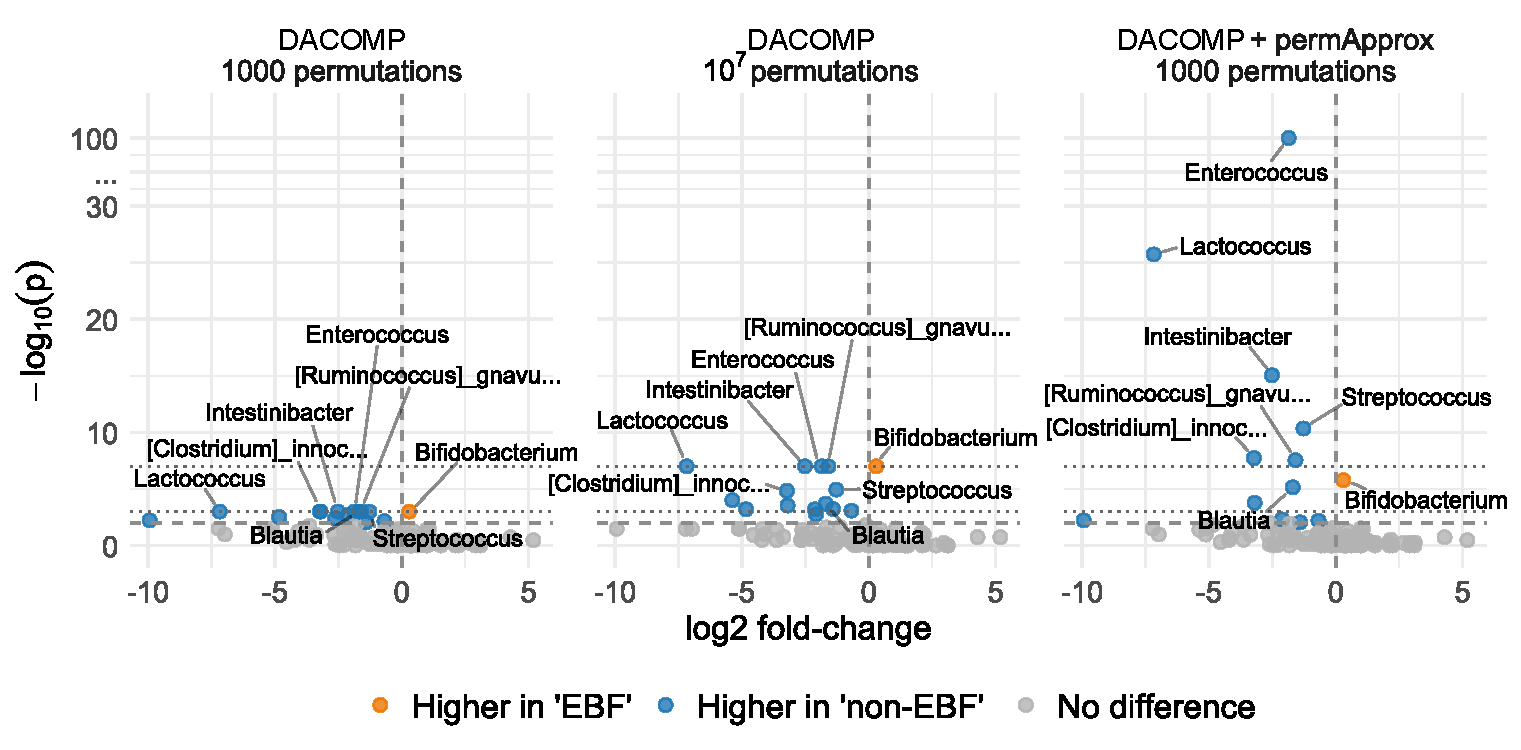
\includegraphics[width=\textwidth]{../ch07_application/figures/08_diff_abundance/thesis_volcano_plot_raw-2.pdf}
	\caption{\label{fig:7app:da:volcano}\textbf{Differential abundance analysis with DACOMP and \texttt{permApprox}.} Volcano plots show log$_2$ fold-changes of mean relative abundance, computed as EBF versus non-EBF, against raw differential abundance $p$-values. The left panel shows empirical DACOMP $p$-values obtained with $1000$ permutations, the middle panel shows empirical DACOMP $p$-values obtained with $10^7$ permutations, and the right panel shows constrained \texttt{permApprox}-refined $p$-values obtained from the $1000$-permutation DACOMP run. Orange points indicate genera with higher mean relative abundance in the EBF group, and blue points indicate genera with higher mean relative abundance in the non-EBF group. Grey points have raw $p$-values above $\alpha=0.01$. The horizontal dashed line marks $\alpha=0.01$ for visual reference. The two dotted horizontal lines indicate the smallest empirical $p$-values attainable with $1000$ and $10^7$ permutations, respectively.}
\end{figure}

After reference selection, DACOMP was run with different permutation budgets to evaluate the effect of finite permutation resolution. The main comparison considered DACOMP with $1000$ permutations, DACOMP with $10^7$ permutations, and DACOMP with $1000$ permutations followed by constrained \texttt{permApprox} refinement. Since the DACOMP statistic is non-negative and larger values indicate stronger evidence against the null hypothesis, $p$-value approximation was performed as a right-tailed problem. The constrained \texttt{permApprox} workflow was applied to the observed and permuted DACOMP statistics using the support-constrained GPD tail approximation described in Chapter~\ref{ch:permapprox}. We used the default configuration described in Section~\ref{sec:6perm:workflow:default_config}, which also corresponds to the default settings of the R implementation. Thus, the empirical $p$-values from the $1000$-permutation DACOMP run were retained in the bulk, whereas small tail $p$-values were refined by constrained GPD approximation.

Figure~\ref{fig:7app:da:volcano} compares the raw $p$-values obtained from the three differential abundance analyses. Raw $p$-values are shown in this plot to display the effect of permutation \text{resolution} and tail approximation without conflating it with multiplicity correction. The corresponding adjusted $p$-values are reported in Appendix Table~\ref{tab:app:7app:diff_abundance_adj_pvalues}. With $1000$ permutations, several taxa reach the empirical lower bound of the permutation $p$-values, so that the strongest effects cannot be distinguished on the $p$-value scale. Increasing the permutation budget to $10^7$ resolves the empirical tail more finely and separates the strongest signals. In this run, \emph{Lactococcus}, \emph{Intestinibacter}, \emph{Enterococcus}, the \emph{[Ruminococcus] gnavus group}, and \emph{Bifidobacterium} appear among the taxa with the smallest raw $p$-values, followed by the \emph{[Clostridium] innocuum group}, \emph{Streptococcus}, and \emph{Blautia}. The constrained \texttt{permApprox} refinement based on only $1000$ permutations identifies largely the same set of taxa as strongest tail signals, but the exact ordering and magnitude of the refined $p$-values differ for some taxa.

\begin{figure}[H]
	\centering
	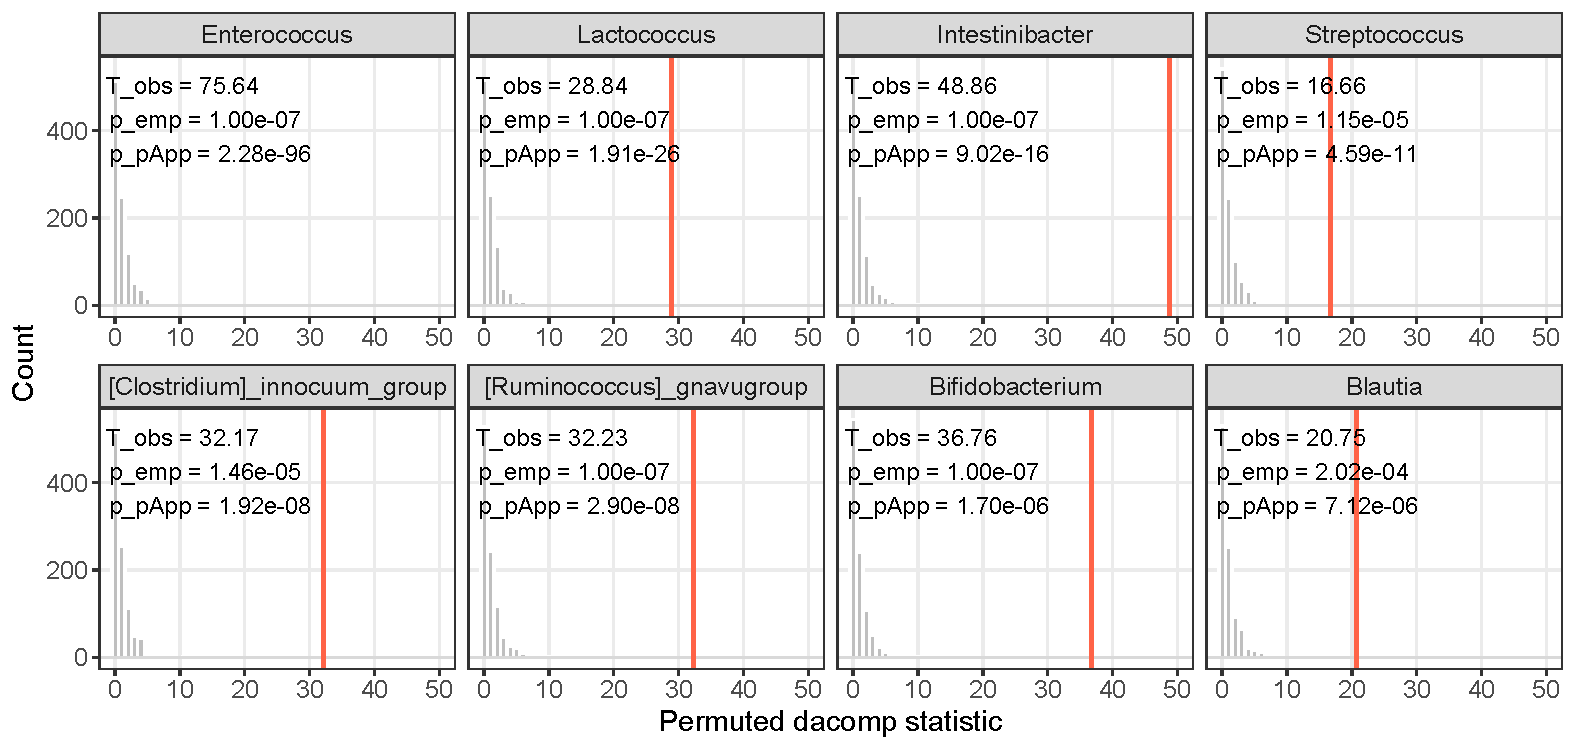
\includegraphics[width=\textwidth]{../ch07_application/figures/08_diff_abundance/thesis_permutation_distribution_plot-1.pdf}
	\caption{\label{fig:7app:da:perm-dist}\textbf{Permutation distributions for selected genera.} Histograms show the permutation distributions of the DACOMP test statistic for the eight genera labeled in Figure~\ref{fig:7app:da:volcano}. Red vertical lines indicate the observed test statistics. The empirical $p$-values shown in the panels are based on the $10^7$-permutation DACOMP run, while the \texttt{permApprox} $p$-values are obtained from the constrained GPD refinement of the $1000$-permutation run. The x-axis is restricted to the interval from $0$ to $50$ for better readability. Observed test statistics outside this range are therefore not visible as vertical lines.}
\end{figure}


The permutation distributions in Figure~\ref{fig:7app:da:perm-dist} illustrate why the $p$-value ranking is not determined by the observed test statistic alone. The panels show the empirical permutation distributions for the eight labeled taxa, together with the observed DACOMP statistic. For \emph{[Clostridium] innocuum group} and the \emph{[Ruminococcus] gnavus group}, the observed DACOMP statistics are almost identical and the permutation distributions have a similar shape, which makes the similar \texttt{permApprox}-refined $p$-values plausible. In contrast, differences between taxa such as \emph{Streptococcus} and \emph{Bifidobacterium} reflect more subtle aspects of the permutation distribution, including the spread of the null distribution, the frequency of large permuted statistics, and the location of the observed statistic relative to the fitted tail. Thus, the refined $p$-value is not a monotone transformation of the observed statistic alone, but combines information from the observed statistic and the estimated tail behavior of the permutation distribution.


The comparison between the empirical $10^7$-permutation $p$-values and the \texttt{permApprox}-refined $p$-values should not be interpreted as an expectation of exact numerical agreement. Both approaches depend on the sampled permutation statistics, and their tail behavior can vary with the random seed. The purpose of the comparison is instead to assess whether the tail approximation translates the observed statistic and the \text{available} permutation distribution into a meaningful refined $p$-value at a much lower computational cost. In this application, the constrained \texttt{permApprox} analysis removes the empirical lower bound of the $1000$-permutation run, separates strong tail signals that are indistinguishable under the smaller permutation budget, and yields results that are broadly coherent with the much more expensive $10^7$-permutation analysis.

%====================================
\subsection{Runtime comparison}
\label{sec:7app:differential-abundance:runtime}
%====================================

The runtime comparison in Table~\ref{tab:7app:da:runtime} illustrates the computational motivation for this refinement. DACOMP with $1000$ permutations required only $1.69$ seconds, but its smallest attainable empirical $p$-value is limited by the coarse permutation grid. Increasing the number of permutations to $10^6$ already required $1675.86$ seconds, corresponding to approximately $27.93$ minutes, while the $10^7$-permutation run required $20963.69$ seconds, corresponding to approximately $5.82$ hours. In contrast, the combined runtime of DACOMP with $1000$ permutations and constrained \texttt{permApprox} refinement was $8.89$ seconds. Thus, compared with the $1000$-permutation DACOMP run alone, the constrained \texttt{permApprox} refinement added only a small absolute runtime overhead, while providing continuous tail $p$-values below the empirical lower bound of the $1000$-permutation analysis.

\begin{table}[!htb]
\centering
\caption{\label{tab:7app:da:runtime}\textbf{Runtime comparison for DACOMP and $p$-value refinement.} Runtime was measured for DACOMP with different permutation budgets and for the combined workflow consisting of DACOMP with $1000$ permutations followed by constrained \texttt{permApprox} refinement. Computations were run on a Linux-based compute node equipped with an Intel Xeon E7-4850 v4 CPU (2.10 GHz) and 170 GB RAM.}
\begin{tabular}{lrrr}
\toprule
Method & Permutations & Runtime (seconds) & Runtime \\
\midrule
DACOMP & $1000$ & $1.69$ & $0.03$ min \\
DACOMP & $10^6$ & $1675.86$ & $27.93$ min \\
DACOMP & $10^7$ & $20963.69$ & $5.82$ h~~~\, \\
DACOMP + \texttt{permApprox} & $1000$ & $8.89$ & $0.15$ min \\
\bottomrule
\end{tabular}
\end{table}

%====================================
\subsection{Descriptive characterization of selected genera}
\label{sec:7app:differential-abundance:selected-genera}
%====================================

The preceding analyses identified eight genera with particularly small differential abundance $p$-values. To relate these formal DACOMP results to the observed data patterns, Figure~\ref{fig:7app:da:rarefied-boxplots} displays the corresponding group-wise distributions on the DACOMP-rarefied count scale. This visualization is descriptive and does not constitute an \text{additional} inferential analysis. Rather, it shows the data representation underlying the DACOMP test statistics and complements the CLR-coordinate violin plots in Figure~\ref{fig:7app:exploration:clr-violin}, which were used for exploratory inspection before formal testing.

For most selected genera, the rarefied-count distributions are consistent with the direction of the differential abundance effects shown in the volcano plot. \emph{Enterococcus}, \emph{Lactococcus}, \emph{Intestinibacter}, \emph{Streptococcus}, the \emph{[Ruminococcus] gnavus group}, and \emph{Blautia} tend to show higher counts among children without EBF, whereas \emph{Bifidobacterium} tends to show higher counts in children with EBF duration of at least two months. Thus, the strongest DACOMP signals largely agree with the descriptive patterns previously observed on the CLR scale, while being evaluated here on the rarefied count representation used for the formal test.

The \emph{[Clostridium] innocuum group} illustrates why differential abundance alone does not fully characterize the nature of a group difference. Its distribution is marked by many zero counts and a pronounced upper tail, rather than by a simple shift in mean counts. This pattern motivates the subsequent differential distribution analysis, which can additionally capture differences in zero prevalence, variability, and tail behavior.

\begin{figure}[!htb]
\centering
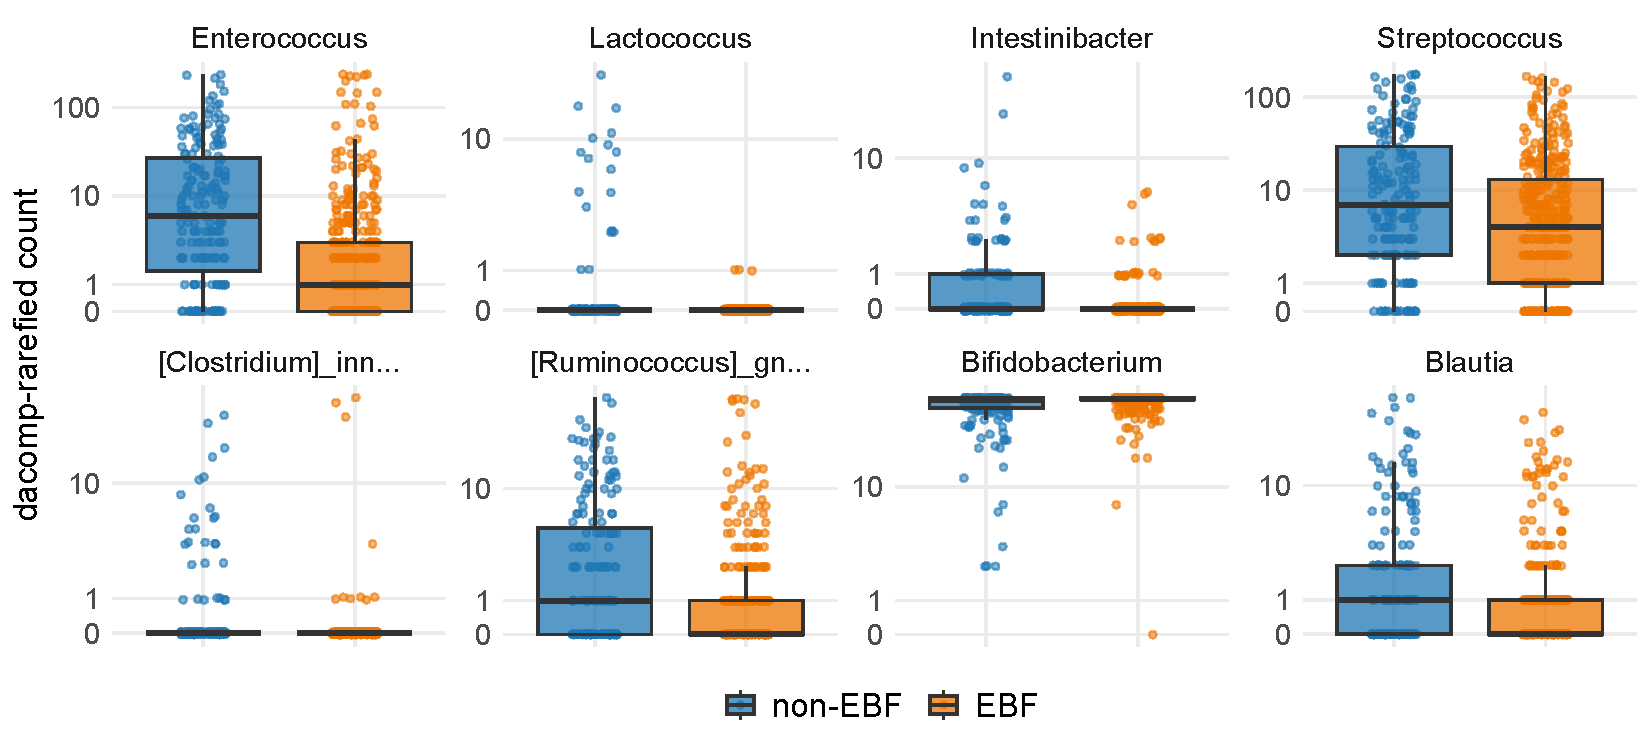
\includegraphics[width=\textwidth]{../ch07_application/figures/08_diff_abundance/thesis_rarefied_count_boxplots_with_zeros-1.pdf}
\caption{\label{fig:7app:da:rarefied-boxplots}\textbf{DACOMP-rarefied counts for selected genera.} Boxplots show group-wise DACOMP-rarefied counts for the eight genera highlighted in the differential abundance volcano plot. Points represent individual samples. The y-axis is displayed on a logarithmic scale, while the axis labels show the original count values. The plot is descriptive and illustrates the group-wise count patterns underlying the DACOMP test statistics.}
\end{figure}

%%%%%%%%%%%%%%%%%%%%%%%%%%%%%%%%%%%%%
\section{Differential distribution analysis}
\label{sec:7app:differential-distribution}
%%%%%%%%%%%%%%%%%%%%%%%%%%%%%%%%%%%%%

%====================================
\subsection{Analysis setup and adapted \texttt{waddR} workflow}
\label{sec:7app:differential-distribution:setup}
%====================================

The differential abundance analysis in the previous section focused on relative abundance shifts of individual genera. As a complementary feature-level analysis, we next assessed whether the marginal distributions of individual genera differed between the two EBF groups. This analysis was performed using the Wasserstein-based \texttt{waddR} framework introduced in Section~\ref{sec:4feature:diffdist}. In contrast to differential abundance testing, differential distribution testing is sensitive not only to location shifts, but also to differences in variability, tail behavior, zero prevalence, and more general distributional shape. The analysis used the binary EBF contrast and the default genus-level data set defined in Section~\ref{sec:7app:default_data}, comparing children without EBF ($n=179$) with children with EBF duration $\ge 2$ months ($n=375$).

Two differential distribution analyses were conducted. The first analysis followed the adapted two-stage approach described in Section~\ref{sec:4feature:diffdist_waddr_microbiome}. In this approach, the zero component was defined on the original count scale and tested whether the prevalence of zero counts differed between the two EBF groups. The non-zero component used the squared 2-Wasserstein statistic on CLR-transformed values, but only among samples in which the corresponding genus had a positive original count. Thus, original counts determined whether an observation entered the non-zero stage, whereas CLR coordinates defined the distributional values being compared. The $p$-values from the zero and non-zero components were combined using Fisher's method to be in line with the original \texttt{waddR} approach. Only the non-zero Wasserstein component was refined using \texttt{permApprox}, because this is the permutation-based part for which the observed and permuted Wasserstein statistics are available.

The second analysis was a one-stage complete-CLR approach. Here, \texttt{waddR} was applied directly to the complete CLR-transformed distributions, including samples with original zero counts through their multiplicative-replacement CLR values. This analysis does not separate zero prevalence from the remaining distributional shape. It is therefore less aligned with the two-stage interpretation of \texttt{waddR}, but it provides a useful contrast because it tests the full CLR-coordinate distribution in a single Wasserstein test. It also makes the connection to the zero-$p$-value problem visible, because all original zeros remain part of the distribution through their replaced CLR values.

For the \texttt{permApprox} refinements, $p$-value approximation was performed as a right-tailed problem, since larger Wasserstein statistics indicate stronger evidence against equality of distributions. The default \texttt{permApprox} configuration described in Section~\ref{sec:6perm:workflow:default_config} was used, with one modification: the approximation threshold was set to $0.01$. This choice was made to align the refinement step with the original \texttt{waddR} tail-approximation rule, which fits a GPD when fewer than $10$ exceedances are observed among $999$ permutations. Thus, the empirical \texttt{waddR} $p$-values were retained outside the extreme tail, whereas small Wasserstein $p$-values were refined by constrained GPD approximation.

%====================================
\subsection{Zero $p$-values and constrained tail approximation}
\label{sec:7app:differential-distribution:zero-pvalues}
%====================================

In the single-cell application of the \texttt{permApprox} study, the original \texttt{waddR} tail approximation produced a considerable number of zero $p$-values \citep{peschel2026permapprox}. In that setting, zero $p$-values arose for two different reasons: some were caused by numerical rounding, whereas others were caused by bounded GPD support under negative shape estimates. The latter case cannot be resolved by numerical post-processing alone and motivated the support-constrained GPD approximation described in Chapter~\ref{ch:permapprox}. In the present PASTURE analysis, this behavior was less pronounced, most likely because the microbiome application has substantially fewer tests and less extreme tail probabilities than the single-cell example.

In the adapted two-stage analysis, no zero $p$-values were observed for the non-zero Wasserstein component. In the one-stage complete-CLR analysis, however, \texttt{waddR} returned zero $p$-values for $5$ of the $116$ taxa for which a finite $p$-value was available, and one additional NA $p$-value. Recomputing the tail $p$-values from the exported observed and permuted Wasserstein statistics with constrained \texttt{permApprox} yielded finite, non-zero $p$-values for all $117$ taxa.


Figure~\ref{fig:7app:dd:pvalue-comparison} shows this zero-$p$-value diagnostic for the one-stage complete-CLR analysis. The left panel shows the $p$-values returned by \texttt{waddR}, including five zero $p$-values and one NA value. The right panel shows the corresponding $p$-values after constrained \texttt{permApprox} refinement. The originally zero and NA values are resolved, and no zero $p$-values remain. This provides a small but relevant example of the zero-$p$-value problem discussed in Chapter~\ref{ch:permapprox}, and illustrates how the constrained GPD approximation can be used to obtain finite tail probabilities for the same observed and permuted test statistics.

\begin{figure}[!htb]
\centering
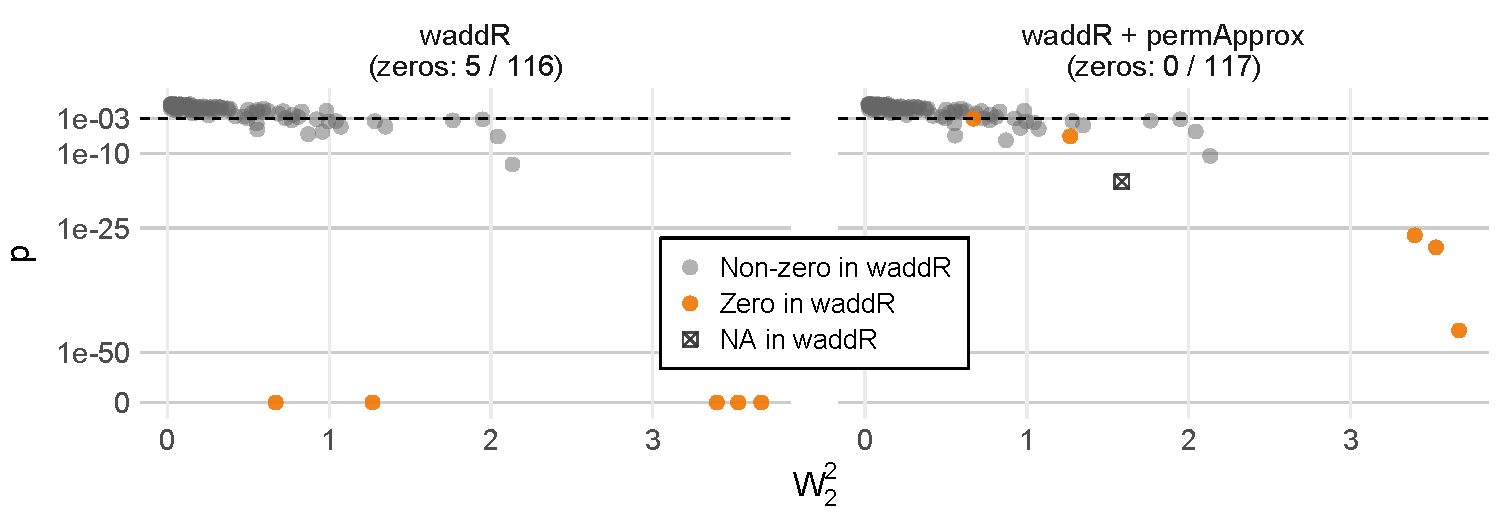
\includegraphics[width=\textwidth]{../ch07_application/figures/09_diff_distribution/thesis_pvalues_complete_clr_waddr_permapprox_constrained_only-1.pdf}
\caption{\label{fig:7app:dd:pvalue-comparison}\textbf{Comparison of \texttt{waddR} and constrained \texttt{permApprox} $p$-values for the one-stage complete-CLR analysis.} Each point represents one genus. The x-axis shows the observed squared 2-Wasserstein statistic $W_2^2$, and the y-axis shows the raw $p$-value on a logarithmic scale. The left panel shows $p$-values returned by \texttt{waddR}, and the right panel shows $p$-values obtained by constrained \texttt{permApprox} refinement from the same observed and permuted Wasserstein statistics. The dashed horizontal line marks the empirical lower bound $1/(B+1)$ for $B=999$ permutations. Zero $p$-values are mapped to the lower plotting boundary for visualization.}
\end{figure}

%====================================
\subsection{Differential distribution results}
\label{sec:7app:differential-distribution:results}
%====================================

The differential distribution results are summarized in Figure~\ref{fig:7app:dd:volcano}. In contrast to a classical volcano plot based on a single effect statistic, each panel displays the native statistic of the corresponding \texttt{waddR} component on the x-axis. For the non-zero \text{distribution} component and the complete-CLR analysis, this is the squared 2-Wasserstein statistic $W_2^2$, and the displayed $p$-values are constrained \texttt{permApprox}-refined $p$-values. For the zero-prevalence component, the x-axis shows the absolute zero-stage statistic $|Z_0|$. For the combined two-stage result, the x-axis shows the combined statistic $C$ obtained from Fisher's method. The y-axis shows the corresponding raw $p$-values on the $-\log_{10}$ scale, while point colors indicate significance after Benjamini--Hochberg adjustment at $\alpha=0.01$. The number of testable taxa differs between panels because not all component statistics could be computed for all genera. For example, \emph{Coprobacillus} had only zero counts in one EBF group and therefore no non-zero Wasserstein statistic. This pattern is instead represented in the zero-prevalence component. Conversely, \emph{Bifidobacterium} had no zero counts and therefore no zero-stage statistic.

The non-zero distribution component identified $15$ of $116$ testable genera as significant after adjustment. These signals include several genera that were already prominent in the differential abundance analysis, such as \emph{Intestinibacter}, \emph{Enterococcus}, \emph{Blautia}, \emph{Streptococcus}, and the \emph{[Ruminococcus] gnavus group}. The zero-prevalence component identified $5$ of $116$ testable genera, including \emph{Lactococcus}, \emph{Haemophilus}, \emph{Leuconostoc}, \emph{Terrisporobacter}, and \emph{Lactobacillus}. Combining the two components yielded $20$ significant genera among $115$ testable genera. Thus, the adapted two-stage result separates distributional differences among originally observed values from differences in the probability of observing a zero count, while the combined statistic summarizes both sources of evidence when both component $p$-values are available.

The one-stage complete-CLR analysis identified $23$ of $117$ genera as significant after adjustment. The strongest signals included \emph{Intestinibacter}, \emph{Enterococcus}, \emph{Lactococcus}, the \emph{[Ruminococcus] gnavus group}, the \emph{[Clostridium] innocuum group}, and \emph{Blautia}. The overlap between the adapted two-stage and complete-CLR approaches indicates that both analyses capture a common set of distributional differences between the EBF groups. At the same time, the approaches are not identical: the two-stage analysis separates zero prevalence from the distribution among originally observed values, whereas the one-stage analysis treats the replaced CLR values of originally zero counts as part of the full distribution. Consequently, the corresponding statistics and $p$-values should not be interpreted as directly interchangeable.

\begin{figure}[!htb]
\centering
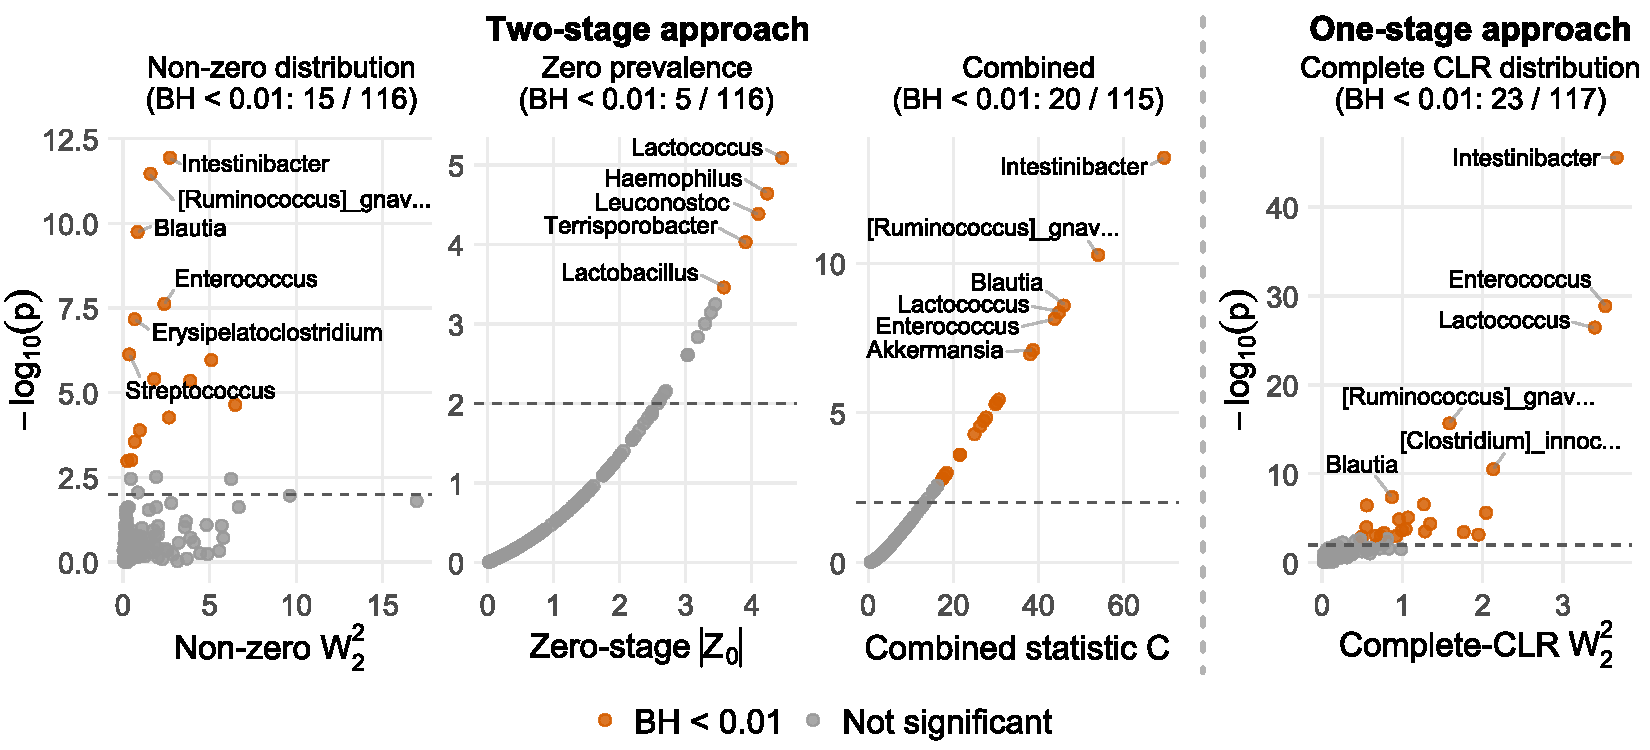
\includegraphics[width=\textwidth]{../ch07_application/figures/09_diff_distribution/thesis_volcano_two_stage_one_stage_native-2.pdf}
\caption{\label{fig:7app:dd:volcano}\textbf{Differential distribution analysis with adapted two-stage and one-stage \texttt{waddR} approaches.} The first three panels show the adapted two-stage approach: the non-zero distribution component, the zero-prevalence component, and the combined result. The fourth panel shows the one-stage complete-CLR analysis. The x-axis displays the native statistic of the respective test component: the squared 2-Wasserstein statistic $W_2^2$ for the non-zero distribution and complete-CLR analyses, the absolute zero-stage statistic $|Z_0|$ for the zero-prevalence analysis, and the combined statistic $C$ for the combined two-stage result. For the two Wasserstein-based panels, $p$-values are constrained \texttt{permApprox}-refined $p$-values. The y-axis shows raw $p$-values on the $-\log_{10}$ scale. Orange points indicate taxa with Benjamini--Hochberg-adjusted $p$-values below $\alpha=0.01$ within the respective panel, and grey points indicate non-significant taxa. The dashed horizontal line marks $\alpha=0.01$ for visual reference. Panel subtitles report the number of significant taxa and the number of taxa for which the respective statistic and $p$-value could be computed. The totals differ between panels because some component statistics are undefined for taxa with only zero counts in one group or no zero counts at all.}
\end{figure}

The adjusted $p$-values for the adapted two-stage components, the combined two-stage analysis, and the one-stage complete-CLR analysis are reported in Appendix Table~\ref{tab:app:7app:diff_distribution_pvalues_all_approaches}. The table confirms the visual impression from Figure~\ref{fig:7app:dd:volcano}: the strongest combined two-stage signals are dominated by genera that also appeared in the differential abundance analysis, but the differential distribution analysis additionally highlights whether the signal is driven by the non-zero distribution, by zero prevalence, or by both. This distinction is useful because a genus can show a similar abundance shift in a differential abundance analysis while differing in the distributional mechanism that produces this shift.

%====================================
\subsection{Distribution diagnostics for selected genera}
\label{sec:7app:differential-distribution:diagnostics}
%====================================

To further inspect the strongest distributional signals, Figure~\ref{fig:7app:dd:diagnostics} shows distribution diagnostics for the four genera with the smallest constrained \texttt{permApprox} $p$-values in the one-stage complete-CLR analysis. The top row shows histograms of CLR coordinates by EBF group, the middle row shows empirical quantile functions, and the bottom row shows the corresponding permutation distributions of the squared Wasserstein statistic. For \emph{Intestinibacter}, \emph{Enterococcus}, \emph{Lactococcus}, and the \emph{[Ruminococcus] gnavus group}, the observed test statistic lies far in the right tail of the permutation distribution. The histograms and quantile functions show that the group differences are not restricted to a single location shift, but also involve differences in the shape and upper tail of the CLR-coordinate distributions. In particular, the non-EBF group tends to show a stronger upper tail for these genera, which is consistent with the differential abundance results and with the exploratory CLR-coordinate visualizations in Section~\ref{sec:7app:feature-level-exploration}.

\begin{figure}[!htb]
\centering
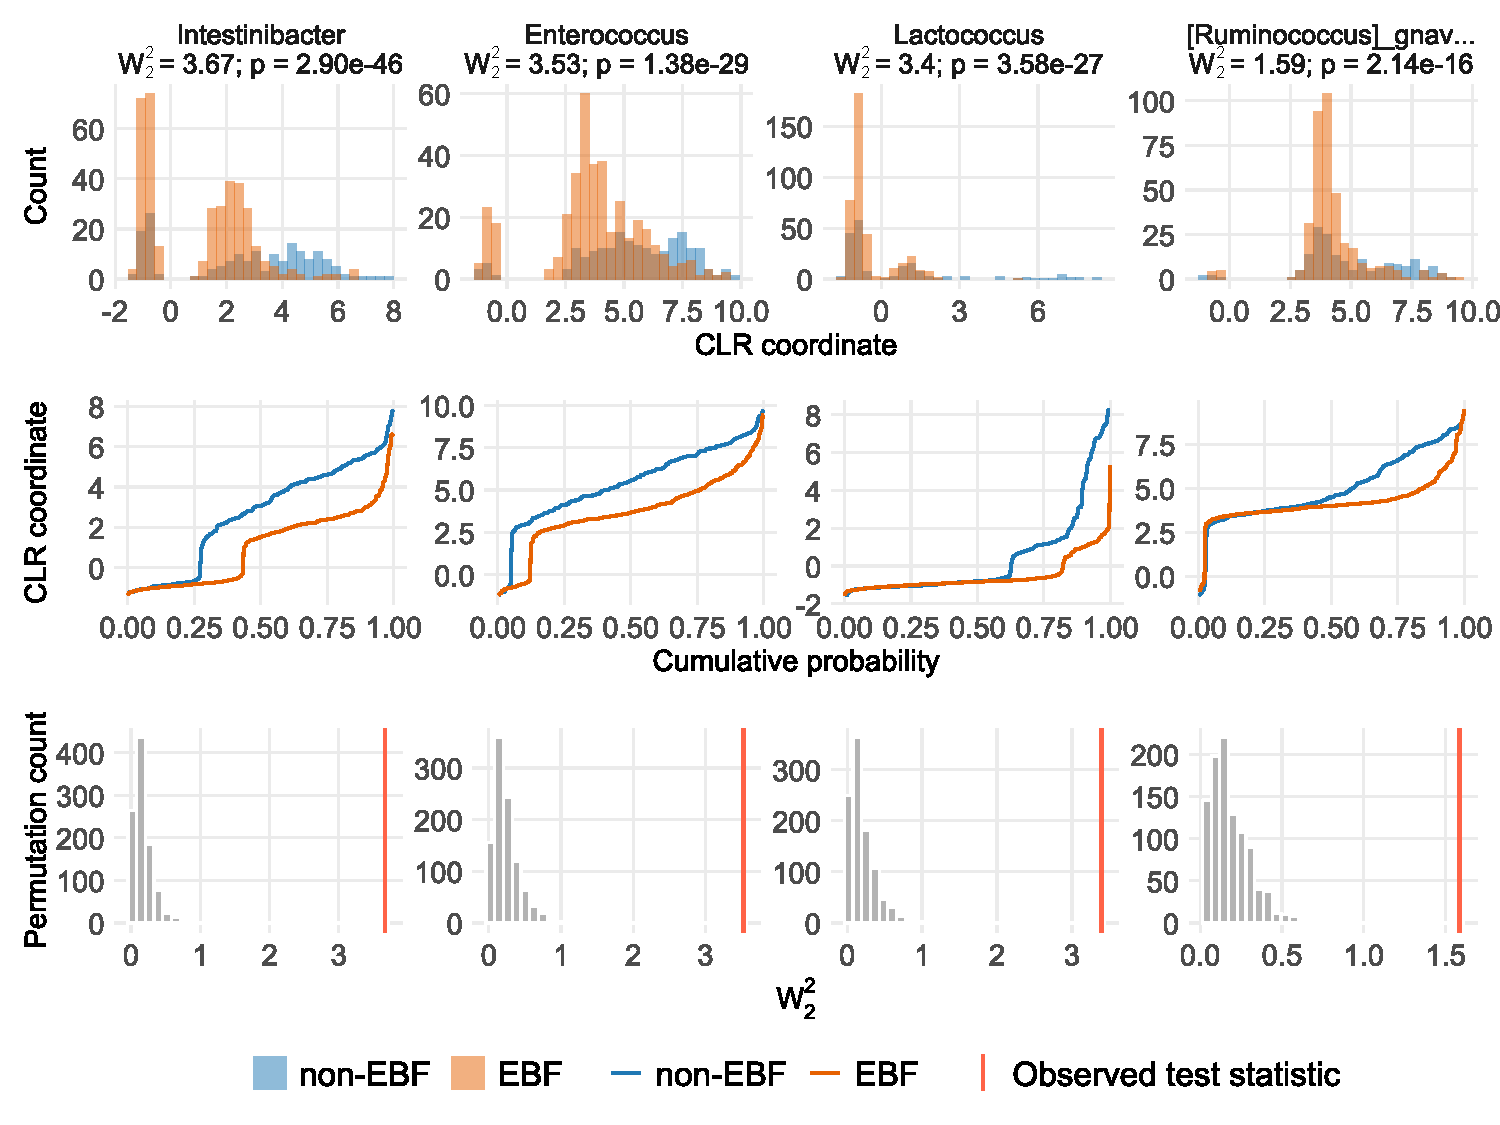
\includegraphics[width=\textwidth]{../ch07_application/figures/09_diff_distribution/thesis_selected_taxa_complete_clr_distribution_diagnostics-2.pdf}
\caption{\label{fig:7app:dd:diagnostics}\textbf{Distribution diagnostics for selected genera in the one-stage complete-CLR analysis.} The figure shows the four genera with the smallest constrained \texttt{permApprox} $p$-values in the one-stage complete-CLR differential distribution analysis. The top row shows histograms of CLR coordinates by EBF group, the middle row shows empirical quantile functions, and the bottom row shows permutation distributions of the squared 2-Wasserstein statistic $W_2^2$. Red vertical lines indicate the observed test statistics. Panel titles report the observed $W_2^2$ statistic and the constrained \texttt{permApprox} $p$-value.}
\end{figure}

%%%%%%%%%%%%%%%%%%%%%%%%%%%%%%%%%%%%%
\section{Network analysis}
\label{sec:7app:networks}
%%%%%%%%%%%%%%%%%%%%%%%%%%%%%%%%%%%%%

The preceding analyses identified genera whose abundance, zero prevalence, or transformed marginal distribution differed between children without EBF and children with EBF duration of at least two months, again referred to as ``non-EBF'' and ``EBF'' groups. These results describe which individual genera show feature-level differences between the two EBF groups, but microbial communities are not merely collections of separate individuals. Genera occur within a joint ecological environment in which their abundances may correlate with those of other community members. Association network analysis addresses this relational aspect by representing genera as nodes and their estimated associations as edges. It thereby shifts attention from marginal, taxon-wise differences to the relationships between genera within the microbial community.

The analysis begins with a baseline network constructed from the complete data set, followed by a comparison of networks estimated separately for the EBF and non-EBF group. Analyzing the baseline network allows us to identify genera with pronounced estimated associations in the complete data set and to characterize the overall network structure of the microbial community. The group comparison assesses whether individual associations or broader network characteristics differ between the EBF groups. In both analyses, we revisit genera highlighted in the preceding sections: we examine whether highly abundant genera occupy notable positions or show distinctive local connectivity in the baseline network, and whether genera with differential abundance or differential distribution are also involved in differential associations between the EBF groups. Such overlap may provide an informative synthesis across analysis targets, although differential abundance or distribution does not imply differential association.

%====================================
\subsection{Baseline association network}
\label{sec:7app:network:baseline}
%====================================

The baseline network was constructed from the complete default data set introduced in Section~\ref{sec:7app:default_data}, which comprises $117$ genera and $592$ samples. Network construction was performed with \texttt{NetCoMi}'s \texttt{netConstruct()} function. As in the preceding analyses, counts were transformed to relative abundances, zeros were replaced by multiplicative replacement, and the resulting compositions were CLR-transformed. Conditional associations were estimated with SPIEC-EASI using the Meinshausen--Bühlmann neighborhood-selection approach described in Section~\ref{sec:5net:net_constr:spieceasi}. A sequence of $30$ regularization parameters was considered, and the final regularization level was selected by the Stability Approach to Regularization Selection using $30$ subsamples and a stability threshold of $0.1$. The directed neighborhood estimates were symmetrized using the average of the two corresponding regression coefficients. The resulting edge weights are therefore symmetrized MB regression coefficients rather than partial correlations. In the following, they are referred to as estimated associations. Their signs indicate the direction of the estimated conditional association, whereas their magnitudes remain specific to the regression-coefficient scale. Because SPIEC-EASI estimates a sparse conditional-dependence structure and selects the regularization level internally by StARS, no additional sparsification was applied.

Figure~\ref{fig:7app:network:association_distribution} summarizes the estimated association matrix. Of the $\binom{117}{2} = 6786$ possible genus pairs, $124$ received a non-zero estimated association, whereas the remaining $6662$ pairs were set to zero by the SPIEC-EASI procedure. The resulting network is therefore sparse, with an edge density of approximately $1.8\%$. The non-zero estimated associations are predominantly positive and modest in magnitude, while negative associations occur less frequently.

\begin{figure}[!htb]
\centering
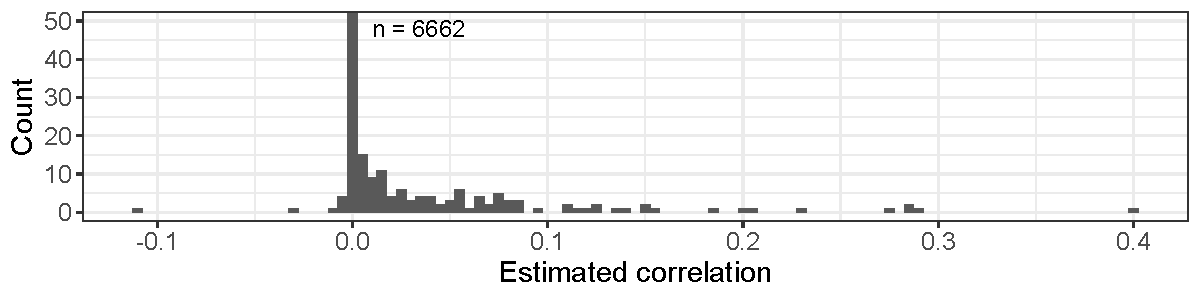
\includegraphics[width=\textwidth]{../ch07_application/figures/10_network_analysis/thesis_single_association_histrogram-1.pdf}
\caption{\textbf{Distribution of estimated associations in the baseline network.} The histogram shows the distribution of estimated associations, including the zero-valued entries resulting from SPIEC-EASI sparsification. The annotation reports the number of associations estimated as zero by the sparsity-inducing procedure.}
\label{fig:7app:network:association_distribution}
\end{figure}

The resulting network was analyzed with \texttt{netAnalyze()} to compute global and node-level characteristics, including component structure, centrality measures, and hub taxa. Figure~\ref{fig:7app:network:baseline_network}, created with \texttt{NetCoMi}'s \texttt{plot()} function, provides an initial visual summary of these characteristics. Node colors represent phylum rather than the detected network clusters because the clustering primarily separates the disconnected components and would therefore add little information beyond the graph layout. Node sizes are proportional to the mean CLR coordinate across samples and therefore summarize the average relative log-ratio abundance of each genus on the transformed scale.

The network consists of one large connected component as well as several smaller components on the right-hand side of the plot. In addition, $31$ of the $117$ genera are singletons. To improve readability, singleton genera are omitted from the visualization unless they are explicitly labeled. The degree distribution shown in Figure~\ref{fig:7app:network:degree_distribution} confirms the heterogeneous connectivity apparent in the network plot: most genera have only few connections, whereas a small number of genera have substantially larger degrees. The network is therefore sparse overall, but its connected structure is dominated by a limited set of highly connected nodes.

The hub taxa identified by \texttt{netAnalyze()} were \emph{8\_Comamonadaceae(F)}, \emph{Blastococcus}, \emph{Brevundimonas}, \emph{Lachnospira}, \emph{Lachnospiraceae ND3007 group}, and \emph{Stenotrophomonas}. Hubs were defined as genera with eigenvector centrality above the empirical $95\%$ quantile. Due to their high connectivity, these taxa also occupy central positions in the network plot. Notably, these genera have comparatively small node sizes, corresponding to low mean CLR coordinates. Their apparent network prominence should therefore be interpreted cautiously, because associations among sparse genera may be sensitive to multiplicative zero replacement before CLR transformation.

In contrast, several genera highlighted in the preceding abundance and differential-distribution analyses show only few and comparatively weak estimated associations, and some occur in smaller connected components. \emph{Bifidobacterium} as the most abundant genus has a few edges but does not have a central position in the network. Its three negative associations with genera highlighted in the preceding analyses are nevertheless notable and suggest a potential relational pattern that complements the marginal feature-level results. The subsequent network comparison examines whether these associations, hub characteristics, and broader network properties differ when the data are analyzed separately for the two EBF groups.

\begin{figure}[H]
\centering
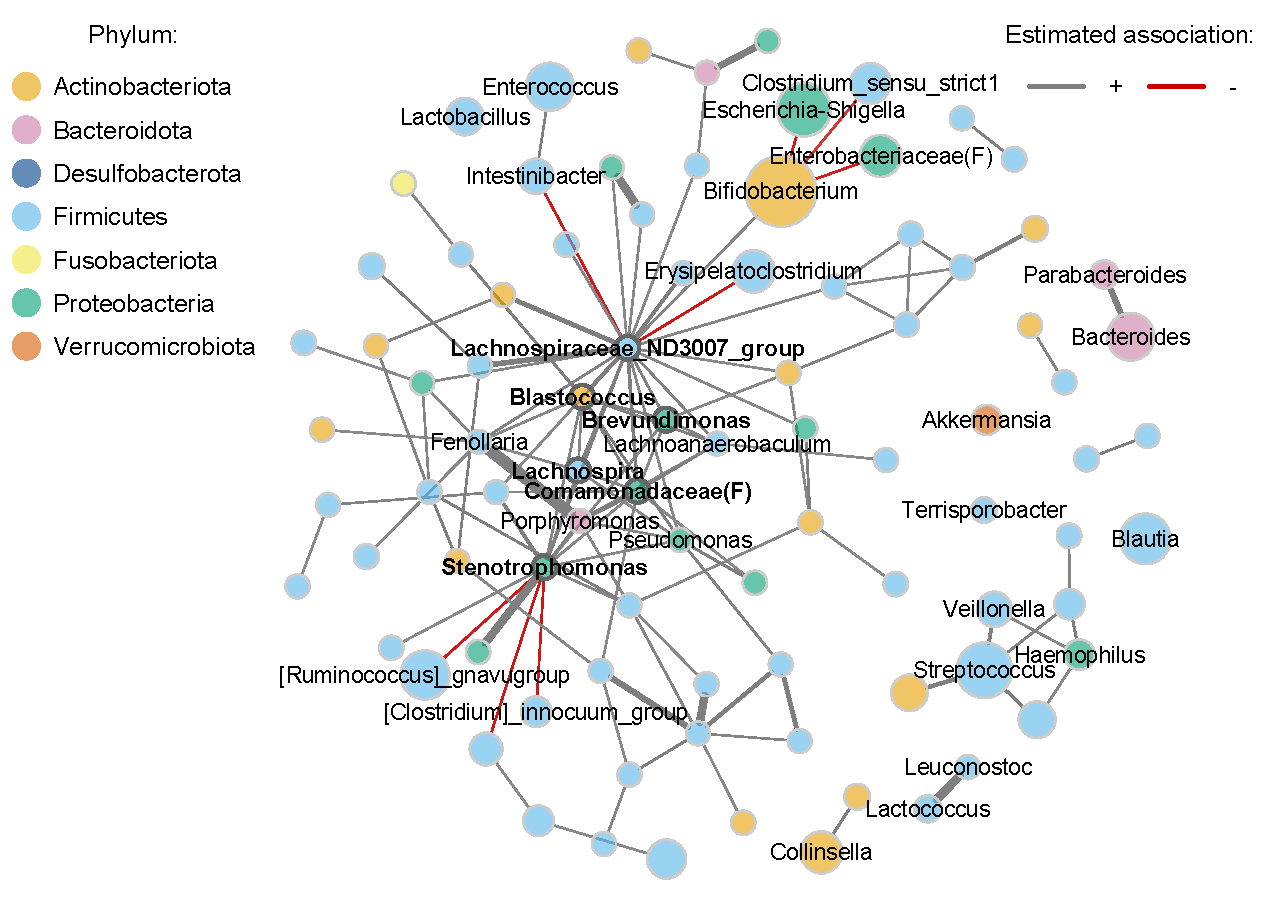
\includegraphics[width=\textwidth]{../ch07_application/figures/10_network_analysis/thesis_single_net_plot_baseline-1.pdf}
\caption{\textbf{Baseline association network for the complete default data set.} Nodes represent genera and are colored according to phylum. Node sizes are proportional to the mean CLR coordinate across samples. Gray and red edges indicate positive and negative estimated SPIEC-EASI associations, respectively. Labels identify highly abundant genera, genera highlighted in the differential abundance or differential distribution analyses, genera with high eigenvector centrality, and the three genera negatively associated with \emph{Bifidobacterium}.}
\label{fig:7app:network:baseline_network}
\end{figure}

\begin{figure}[H]
\centering
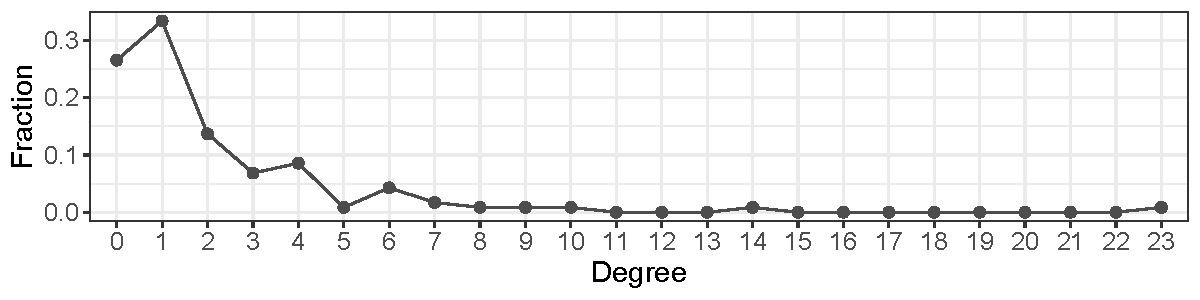
\includegraphics[width=\textwidth]{../ch07_application/figures/10_network_analysis/thesis_single_degree_distribution-1.pdf}
\caption{\textbf{Degree distribution of the baseline association network.} The degree of a genus is the number of genera to which it is connected, i.e., has a non-zero estimated association.}
\label{fig:7app:network:degree_distribution}
\end{figure}

\begin{figure}[H]
\centering
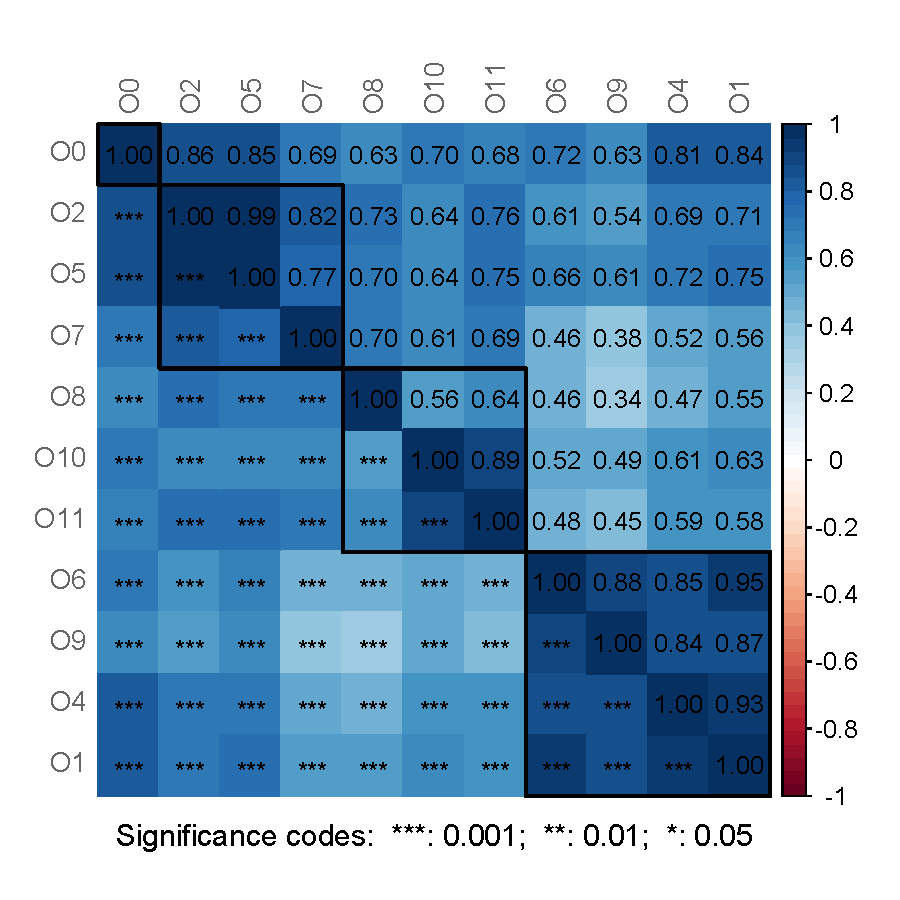
\includegraphics[width=0.9\textwidth]{../ch07_application/figures/10_network_analysis/thesis_single_gcm-1.pdf}
\caption{\textbf{Graphlet correlation matrix of the baseline association network.} Entries show Spearman correlations between graphlet orbit counts across genera. Significance symbols refer to tests of non-zero correlation performed with Fisher's z-test.}
\label{fig:7app:network:baseline_gcm_heatmap}
\end{figure}

Finally, Figure~\ref{fig:7app:network:baseline_gcm_heatmap} shows the corresponding graphlet correlation matrix (GCM). The matrix is dominated by strong positive correlations between graphlet orbit counts, indicating that genera participating frequently in one orbit also tend to participate frequently in several others. Compared with the GCMs of the standard networks shown in Figures~\ref{fig:5net:net_analysis:gcm_example} and \ref{fig:app:5net:gcm_network_models}, the PASTURE GCM is most similar overall to the standard Barabási--Albert (BA) network. This is notable because the modified BA network in Figure~\ref{fig:5net:net_analysis:gcm_example} was deliberately augmented with peripheral nodes to obtain a structure that appears more similar to empirical networks. In that modified network, the additional peripheral nodes weaken the correlations of certain peripheral orbit roles, in particular O6 and O9, with the remaining orbit counts. However, the local role of peripheral nodes differs between the two networks. In the modified BA network, the added peripheral nodes frequently occur in triangle- and star-related graphlets, which weakens the correlations of orbits O6 and O9 to other orbits. In the PASTURE network, by contrast, peripheral genera more often occupy endpoint positions in chain-like graphlets. 

The PASTURE GCM also shares some features with the stochastic block model, including pronounced positive correlations among orbit counts in the lower-right part of the matrix. At the same time, the strong correlation block involving O0, O2, O5, and O7 is more pronounced in the stochastic block model heatmap than that of the PASTURE network. Thus, the PASTURE GCM combines features visible in several standard network models, however, these similarities should not be interpreted as evidence that the microbial association network follows a particular generative network model. Rather, the GCM provides a descriptive summary of local network structure that complements the degree and centrality measures and serves as an additional reference for the subsequent comparison of the EBF-group-specific networks.

%====================================
\subsection{Sensitivity to network-construction choices}
\label{sec:7app:network:sensitivity}
%====================================

The baseline network revealed several pronounced estimated associations among genera with low mean CLR coordinates. As these genera were also characterized by high zero fractions before we replaced them, their apparent network prominence may be sensitive to choices made during preprocessing. We therefore examined how the estimated network changes under alternative preprocessing and association-estimation approaches. First, we considered stronger prevalence filters, which remove low-prevalence genera before network construction and allow us to assess which associations among the remaining genera are retained. Second, we compared alternative zero-replacement procedures as a less restrictive approach to handling sparse taxa. Finally, we consider alternative association-estimation methods to investigate how strongly the estimated network depends on the selected measure.

Throughout this subsection, the network constructed in Section~\ref{sec:7app:network:baseline} is used as the baseline network. To facilitate visual comparison, all alternative networks use the same node layout and labeling as the baseline network whenever the corresponding genera are retained.

%------------------------------------
\subsubsection{Prevalence filtering}
\label{sec:7app:network:sensitivity:prevalence}
%------------------------------------

The baseline network was constructed after applying the $1\%$ prevalence filter. Figure~\ref{fig:7app:network:combined_prevalence} compares this network with networks estimated after applying more stringent prevalence filters of $5\%$ and $10\%$. The same preprocessing, SPIEC-EASI MB estimation procedure, and StARS-based regularization selection were used in all three analyses. Only the set of retained genera differed.

The more stringent filters remove the low-prevalence genera that formed several of the highly connected regions in the baseline network. Consequently, these genera and their estimated associations no longer appear in the networks constructed after $5\%$ and $10\%$ filtering. At the same time, several associations among more prevalent genera are recovered. For example, the component centered on \emph{Streptococcus} in the lower-right part of the network remains visible under both stronger filters. Two negative associations involving \emph{Bifidobacterium} are also retained, namely those with \emph{Clostridium sensu stricto 1} and \emph{Enterobacteriaceae(F)}.

The stronger filters therefore reduce the uncertainty associated with associations involving extremely sparse taxa, but this comes at a substantial loss of taxonomic information. Of the $117$ genera retained after $1\%$ filtering, only $58$ remain after applying the $5\%$ filter and $41$ after applying the $10\%$ filter. Thus, stricter filtering yields smaller and visually simpler networks, but it also excludes many genera that may be biologically relevant and that contributed to the structure of the baseline network.

\begin{figure}[!htb]
\centering
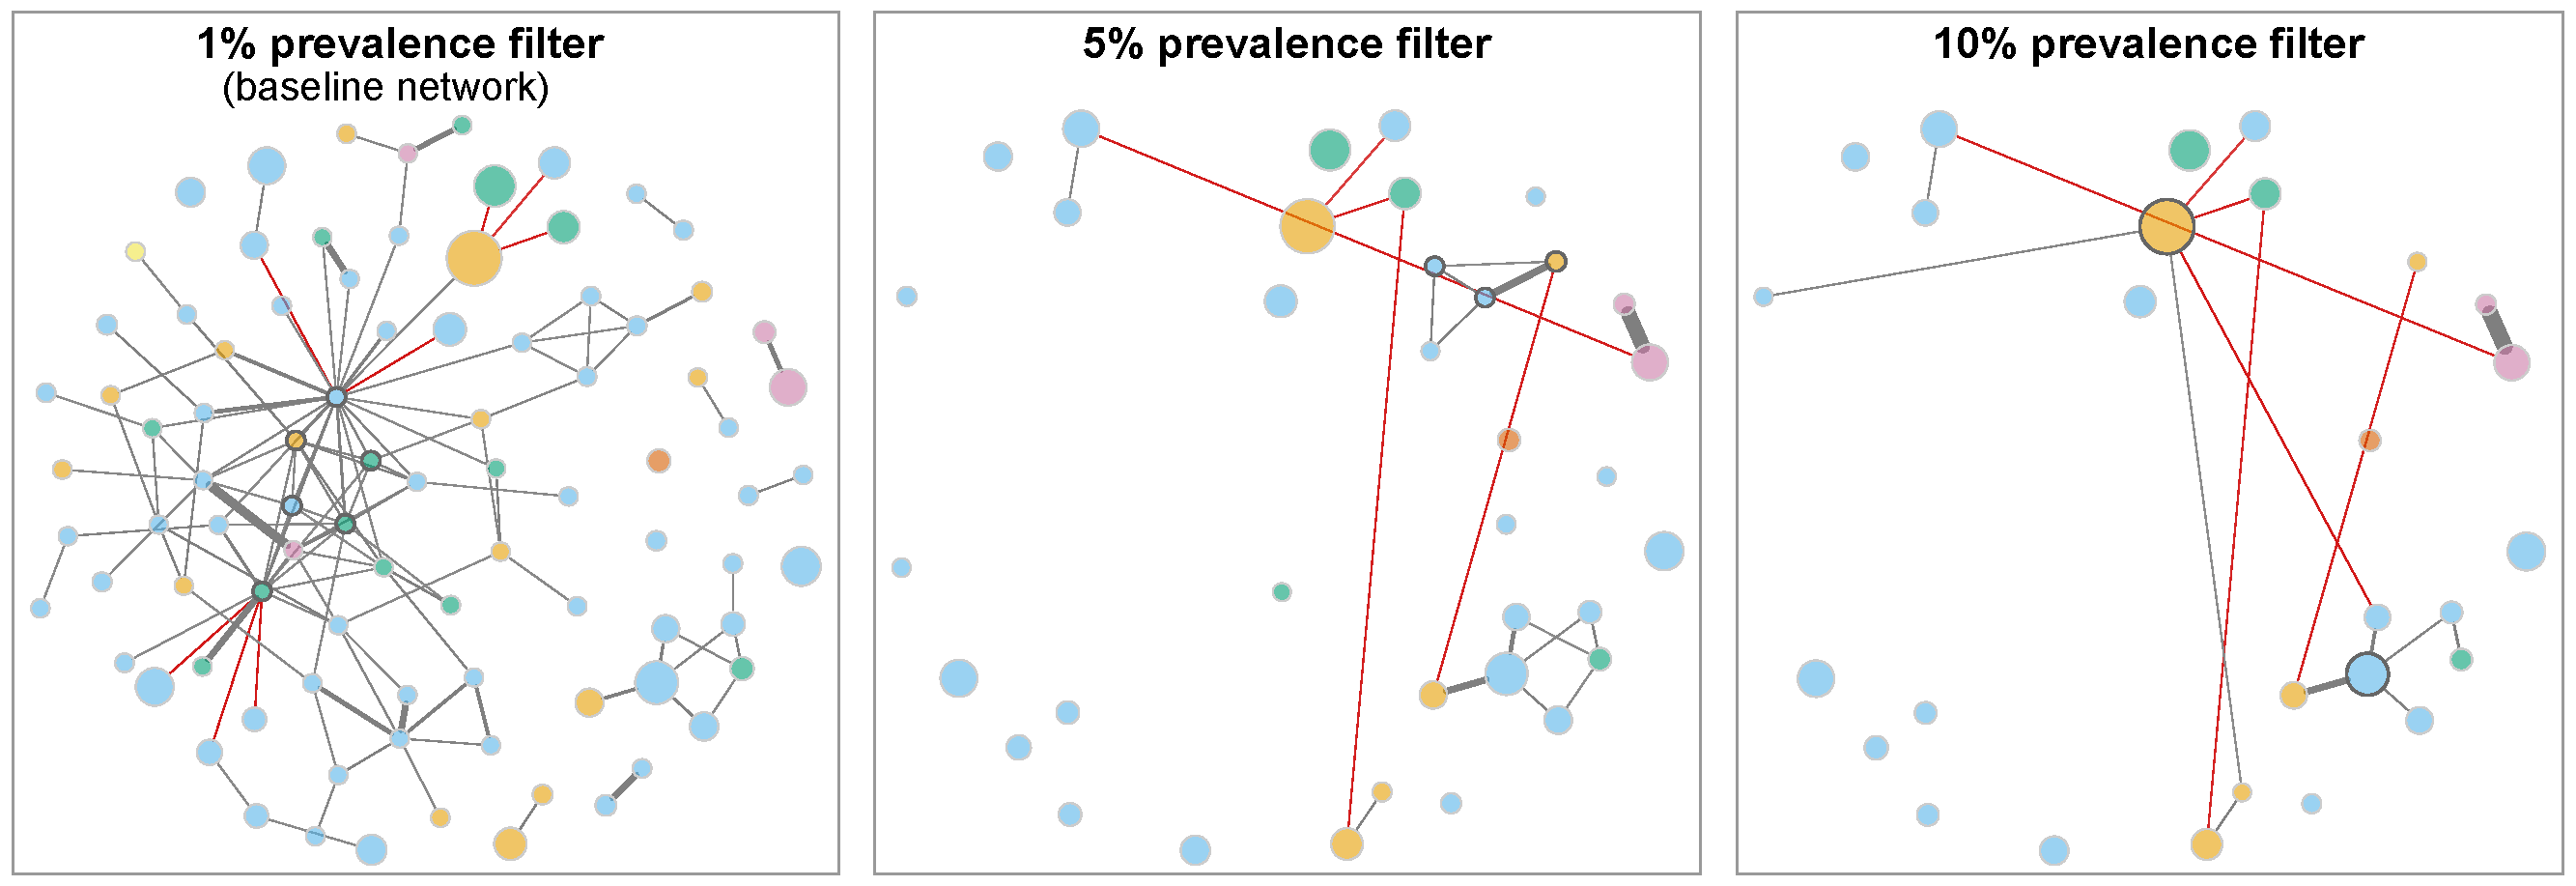
\includegraphics[width=\textwidth]{../ch07_application/figures/10_network_analysis/thesis_combined_networks_prevalence.pdf}
\caption{\textbf{Association networks obtained with different prevalence filters.} Networks were estimated from data filtered at $1\%$, $5\%$, and $10\%$ prevalence using the same preprocessing and SPIEC-EASI MB workflow. The $1\%$ network corresponds to the baseline network. Nodes represent genera and are colored according to phylum, whereas node sizes are proportional to the mean CLR coordinate across samples. Node positions and labels were kept consistent across panels where possible to facilitate comparison. Genera removed by a stricter prevalence filter are not shown in the corresponding network.}
\label{fig:7app:network:combined_prevalence}
\end{figure}

%------------------------------------
\subsubsection{Zero replacement}
\label{sec:7app:network:sensitivity:zero_repl}
%------------------------------------

The baseline network contains several pronounced associations among genera with low mean CLR coordinates and high zero fractions. One possible explanation is that these associations are partly induced by the zero-replacement step preceding CLR transformation. In particular, multiplicative replacement assigns the same small replacement value to zero entries when a common detection limit is used. Genera that are absent in many of the same samples may therefore receive highly similar imputed values, which can affect subsequent association estimation. This possibility cannot be assessed from the baseline network alone. We therefore repeated network construction with three alternative zero-replacement procedures while retaining the $1\%$ prevalence filter, CLR transformation, SPIEC-EASI MB estimation, and all remaining network-construction settings.

As a simple diagnostic approach, zeros were replaced by independently drawn pseudo-counts between zero and the upper bound used for multiplicative replacement, namely $0.65$ times the minimum non-zero relative abundance. Only zero entries were modified. This approach is not intended as a principled imputation method, but deliberately disrupts the common replacement pattern induced by assigning identical pseudo-counts to zero entries. As shown in the left panel of Figure~\ref{fig:7app:network:combined_zero_repl}, the dense region of associations among low-abundance genera disappears under this procedure. This result indicates that these associations are sensitive to the particular treatment of zero entries.

\begin{figure}[H]
	\centering
	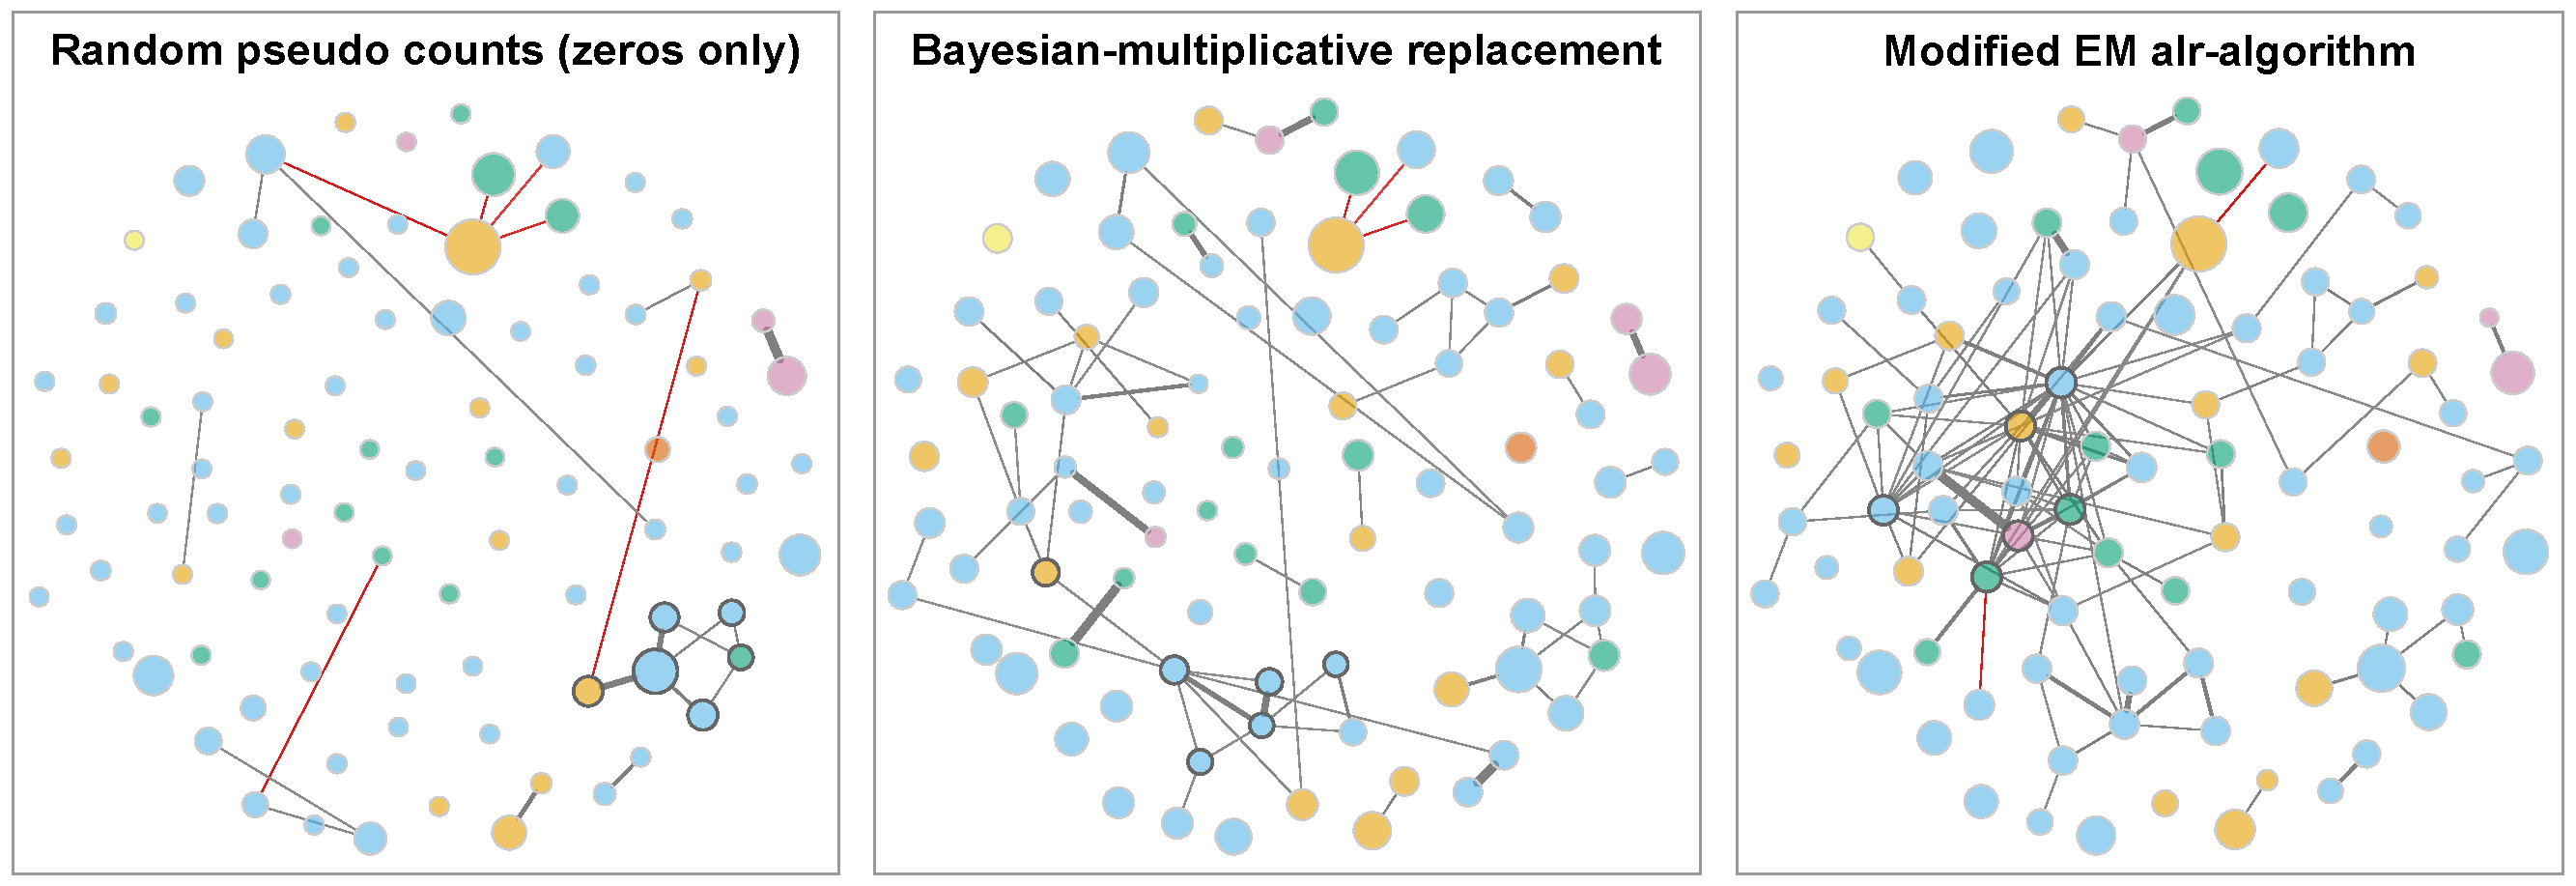
\includegraphics[width=\textwidth]{../ch07_application/figures/10_network_analysis/thesis_combined_networks_zero_repl.pdf}
	\caption{\textbf{Association networks obtained with alternative zero-replacement procedures.} All networks were constructed from the data set filtered at $1\%$ prevalence using CLR transformation and the same SPIEC-EASI MB workflow as for the baseline network. The panels show results after random pseudo-count replacement of zero entries, Bayesian-multiplicative replacement, and the modified EM alr-algorithm, respectively. Nodes represent genera and are colored according to phylum, whereas node sizes are proportional to the mean CLR coordinate across samples. Node positions and labels were kept consistent with the baseline network where possible to facilitate comparison.}
	\label{fig:7app:network:combined_zero_repl}
\end{figure}


The second approach used Bayesian-multiplicative replacement, as described in Section~\ref{sec:2micro:zeros}. This method models the observed counts using a Dirichlet-multinomial framework and derives replacement values from a posterior distribution whose Dirichlet parameters are estimated from the complete count matrix. In contrast to the random pseudo-count approach, it therefore provides a model-based treatment of count zeros while remaining computationally inexpensive. The corresponding network in the center panel of Figure~\ref{fig:7app:network:combined_zero_repl} likewise does not reproduce the highly connected low-abundance region observed in the baseline network. At the same time, several associations among more prevalent genera remain visible, including the component centered on \emph{Streptococcus}.

Finally, the modified EM alr-algorithm described in Section~\ref{sec:2micro:zeros} was applied. This procedure imputes zeros through an expectation-maximization algorithm on additive log-ratio coordinates and explicitly incorporates the estimated covariance structure. Here, it produced a markedly denser network and retained several associations among low-abundance genera, as shown in the right panel of Figure~\ref{fig:7app:network:combined_zero_repl}. Thus, accounting for multivariate dependence during imputation does not necessarily reduce sensitivity to sparse taxa and may itself induce substantial changes in the inferred network.

Overall, the comparison demonstrates that the apparent prominence of low-abundance genera in the baseline network depends strongly on the chosen zero-replacement method. The random pseudo-count and Bayesian-multiplicative approaches weaken this pattern, whereas the modified EM alr-algorithm yields an even denser low-abundance subnetwork. These results do not identify a uniquely correct replacement procedure, but they show that associations involving highly sparse genera should be interpreted cautiously. The next subsection therefore examines whether this sensitivity persists when the association-estimation method itself is changed.


We additionally considered a variant of multiplicative replacement in which the detection limit was determined separately for each sample rather than globally across the complete data set. Specifically, the replacement value in each sample was based on $0.65$ times the smallest non-zero relative abundance observed in that sample. The corresponding network is not shown here but is provided in the thesis repository. This analysis produced an even denser subnetwork among the low-abundance hub taxa than the baseline procedure. Such behavior is consistent with the fact that the replacement value now varies across samples and is partly determined by sample-specific sequencing depth and sparsity. When several rare genera are simultaneously absent from the same sample, they receive the same sample-specific replacement value and may therefore share an artificial abundance pattern across samples after CLR transformation. The result further illustrates that associations among highly sparse genera can be strongly affected not only by whether zeros are replaced, but also by how the replacement value is defined.

%------------------------------------
\subsubsection{Association estimation}
\label{sec:7app:network:sensitivity:association}
%------------------------------------

Two further approaches are particularly relevant when the aim is to make network estimation less sensitive to potentially zero-induced spurious associations: the sparse-plus-low-rank (SLR) decomposition proposed by \citet{kurtz2019disentangling} and implemented in \texttt{SpiecEasi}, and SPRING \citep{yoon2019microbial}, which is implemented in an R package of the same name. As explained in Section~\ref{sec:5net:net_construction}, both methods estimate sparse conditional-dependence networks, but they address different potential sources of spurious association. The SLR approach represents the inverse covariance structure as the sum of a sparse component and a low-rank component, where the latter captures variation attributable to a small number of unobserved factors. SPRING, in contrast, estimates a latent correlation matrix under a truncated Gaussian copula model and avoids external zero replacement by using the modified CLR transformation described in Section~\ref{sec:2micro:clr_with_zeros:mCLR}.

For SPIEC-EASI SLR estimation, candidate ranks from $2$ to $5$ were considered for the low-rank component, and the rank minimizing the extended Bayesian information criterion (eBIC) was selected. We used $\gamma = 0.5$, a commonly used conservative default for eBIC-based high-dimensional graph selection. The resulting eBIC values and heatmaps of the fitted low-rank components are provided in the thesis repository. The remaining SPIEC-EASI settings were identical to those of the baseline analysis, with a $\lambda$ path of length $30$, $30$ StARS subsamples, and a stability threshold of $0.1$. For SPRING, the same StARS settings were used. No additional sparsification was applied because both procedures incorporate stability-based model selection.

Figure~\ref{fig:7app:network:combined_association} compares the baseline SPIEC-EASI MB network with the networks estimated using SPIEC-EASI SLR and SPRING. The baseline network is repeated in the left panel to facilitate comparison. Both alternative approaches yield markedly different edge sets from the MB network and from the preceding preprocessing-based sensitivity analyses. In particular, the SLR network contains many negative estimated associations, whereas the SPRING network shows a distinct mixture of positive and negative edges. Importantly, the additional associations in both networks are primarily located among genera with moderate or high mean CLR coordinates rather than among the low-abundance genera that formed the highly connected region of the baseline network. This pattern is consistent with the purpose of both approaches: the SLR model can attribute shared broad-scale variation to the low-rank component, whereas SPRING avoids the common pseudo-value structure introduced by multiplicative zero replacement.

The common layout in Figure~\ref{fig:7app:network:combined_association} is useful for locating differences relative to the baseline network, but it does not necessarily provide the clearest visualization of either alternative network. Network plots based on their respective spring layouts, including the corresponding labels and annotations, are therefore provided in Appendix~\ref{sec:app:7app:net_analysis}.

\begin{figure}[!htb]
\centering
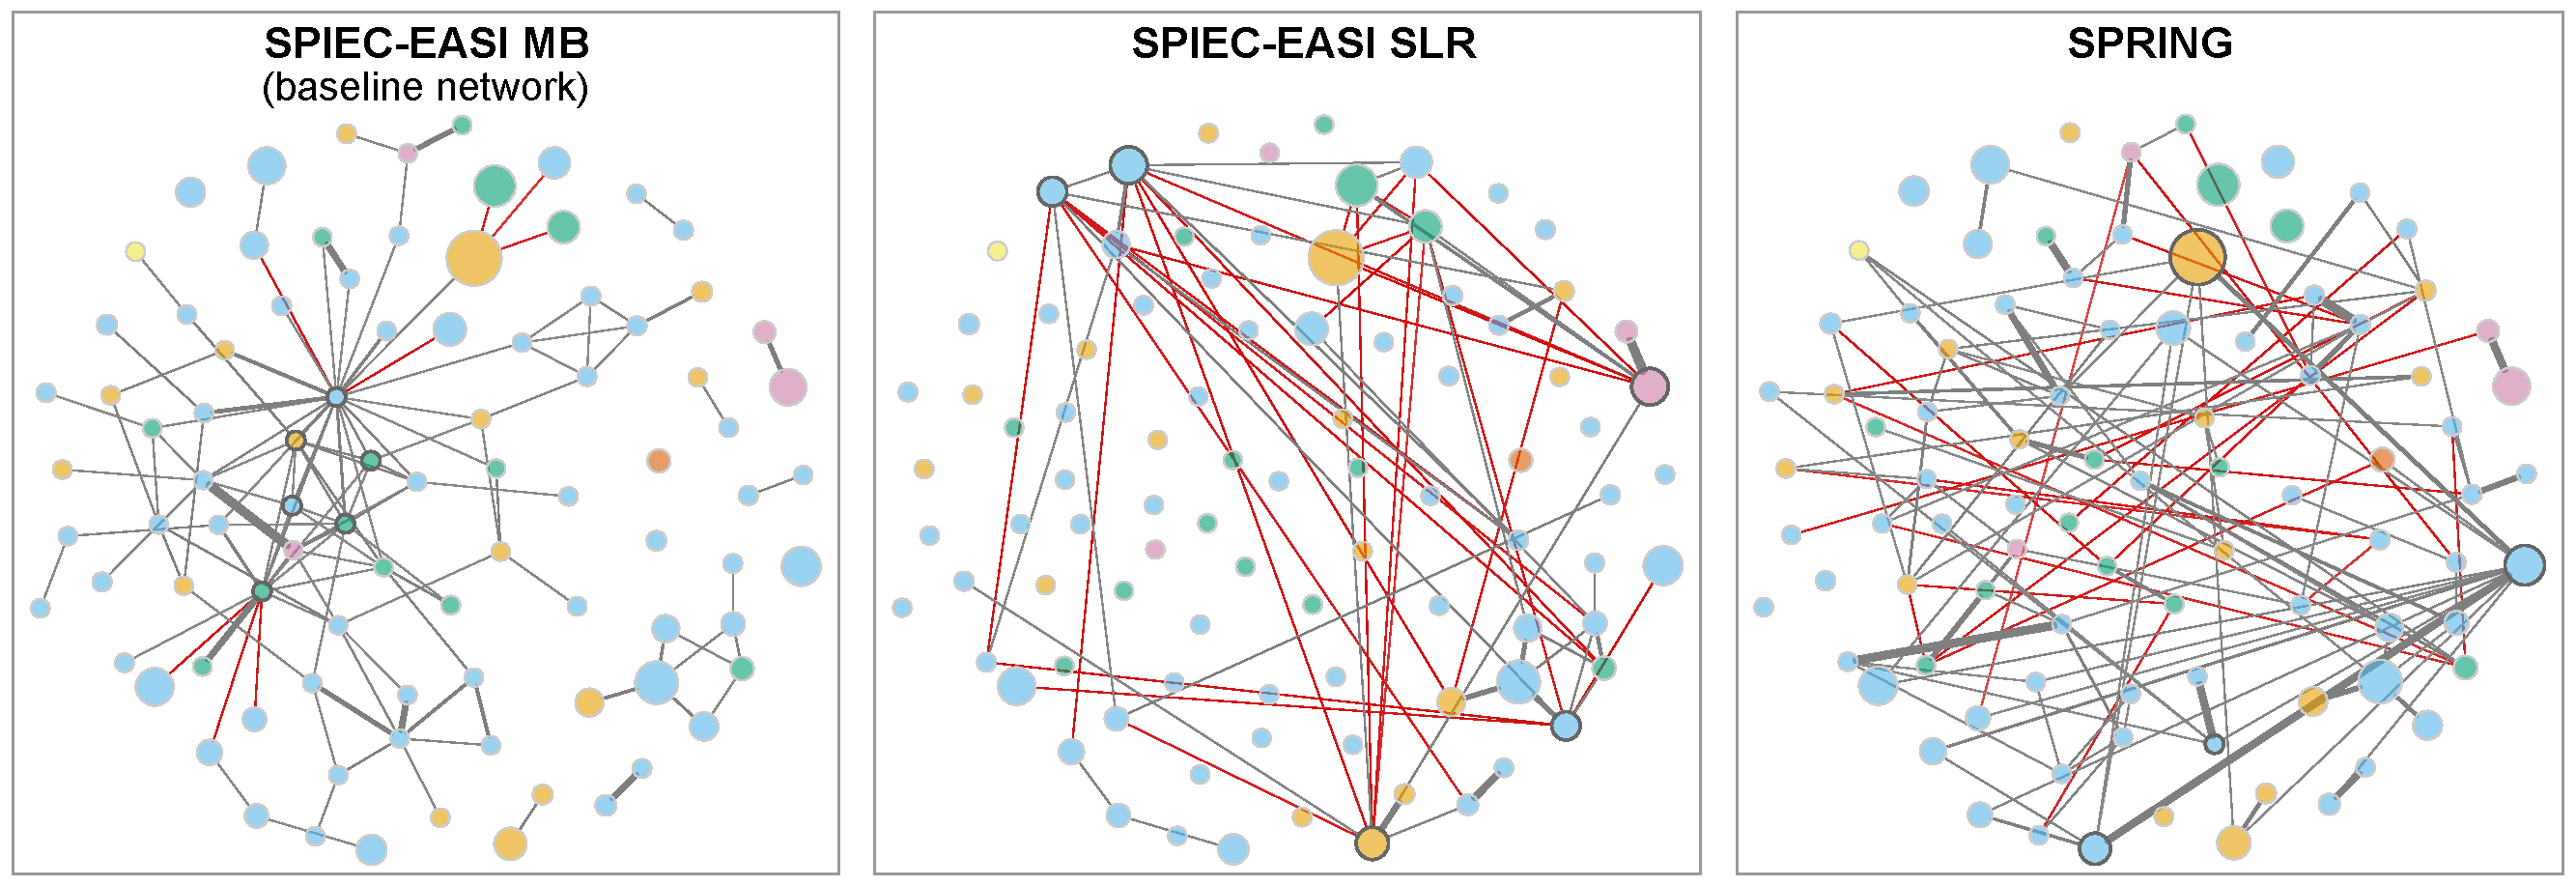
\includegraphics[width=\textwidth]{../ch07_application/figures/10_network_analysis/thesis_combined_networks_association.pdf}
\caption{\textbf{Association networks estimated with alternative conditional-dependence methods.} The left panel shows the SPIEC-EASI MB baseline network. The center and right panels show networks estimated using SPIEC-EASI sparse-plus-low-rank estimation and SPRING, respectively. Node positions, labels, colors, and sizes were kept consistent across panels to facilitate comparison. Nodes represent genera and are colored according to phylum, whereas node sizes are proportional to the mean CLR coordinate across samples. Gray and red edges indicate positive and negative estimated associations, respectively.}
\label{fig:7app:network:combined_association}
\end{figure}

The large number of negative associations estimated by the sparse-plus-low-rank approach also motivates an alternative network representation. In the \emph{signed} network used above, strong negative associations correspond to large dissimilarities and \text{therefore} receive low edge weights. We therefore additionally constructed an unsigned SLR network, as described in Section~\ref{sec:5net:net_construction}. Under this representation, positive and negative associations of large magnitude are both treated as strong connections. Figure~\ref{fig:7app:network:spiecEasi_slr_unsigned_net} shows that several associations involving genera highlighted in the preceding analyses become visually prominent. In particular, \emph{Bacteroides} is strongly positively associated with \emph{Parabacteroides} and strongly negatively associated with \emph{Enterococcus}. The negative associations of \emph{Bifidobacterium} with \emph{Enterobacteriaceae(F)} and \emph{Clostridium sensu stricto 1} are also retained. These patterns should be interpreted as conditional associations estimated under the SLR model rather than as direct biological interactions.

\begin{figure}[!htb]
\centering
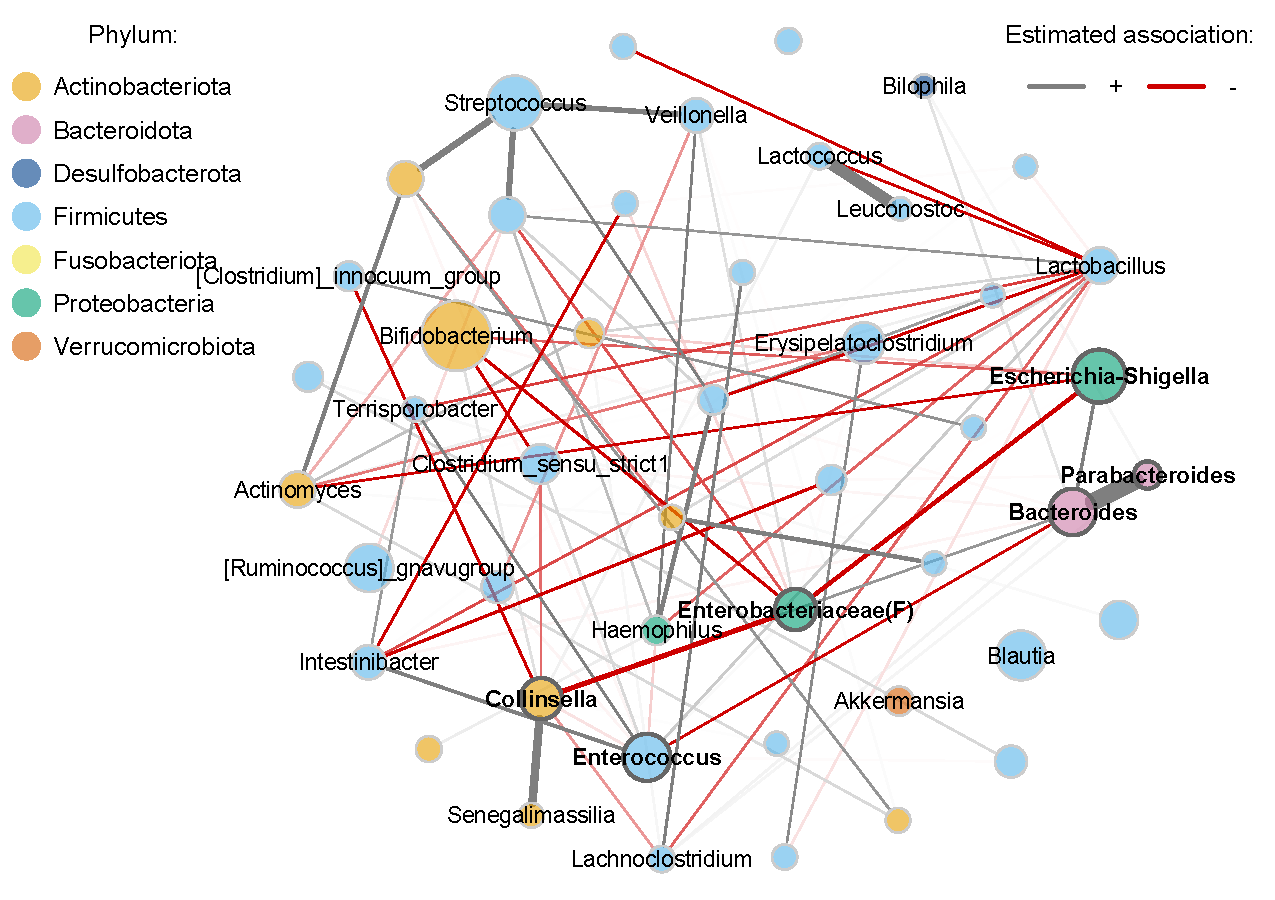
\includegraphics[width=\textwidth]{../ch07_application/figures/10_network_analysis/thesis_single_net_plot_slr_us-1.pdf}
\caption{\textbf{Unsigned network based on SPIEC-EASI SLR estimation.} The network is based on the same sparse-plus-low-rank (SLR) association estimates shown in Figure~\ref{fig:7app:network:combined_association}, but uses the unsigned association-to-similarity transformation. Positive and negative estimated associations with large magnitude therefore both contribute strongly to network connectivity. Nodes represent genera and are colored according to phylum. Node sizes are proportional to the mean CLR coordinate across samples. Gray and red edges indicate positive and negative estimated associations, respectively.}
\label{fig:7app:network:spiecEasi_slr_unsigned_net}
\end{figure}

%------------------------------------
\subsubsection{Persistent edges across sensitivity analyses}
\label{sec:7app:network:sensitivity:persistent_edges}
%------------------------------------

The preceding analyses demonstrated that the estimated network structure changes substantially when prevalence filtering, zero replacement, or association estimation are modified. To summarize the resulting edge-set overlap, UpSet plots were generated separately for the three types of sensitivity analysis.

 Figure~\ref{fig:7app:network:upset_association} shows the comparison across association-estimation methods. The corresponding overlap summaries for prevalence filtering and zero replacement are provided in the thesis repository.
The three association-estimation approaches share only $11$ edges, despite containing between $124$ and $186$ edges in total. This limited overlap reinforces the visual impression that the inferred association structure depends strongly on the selected estimation method. Nevertheless, several taxon pairs occur repeatedly across the different analyses. To identify associations that are comparatively robust to the examined network-construction choices, we considered the $8$ distinct signed networks obtained across all sensitivity analyses: the baseline network, the two networks based on stronger prevalence filters, the three alternative zero-replacement networks, and the two networks based on alternative association-estimation methods.

\begin{figure}[!htb]
\centering
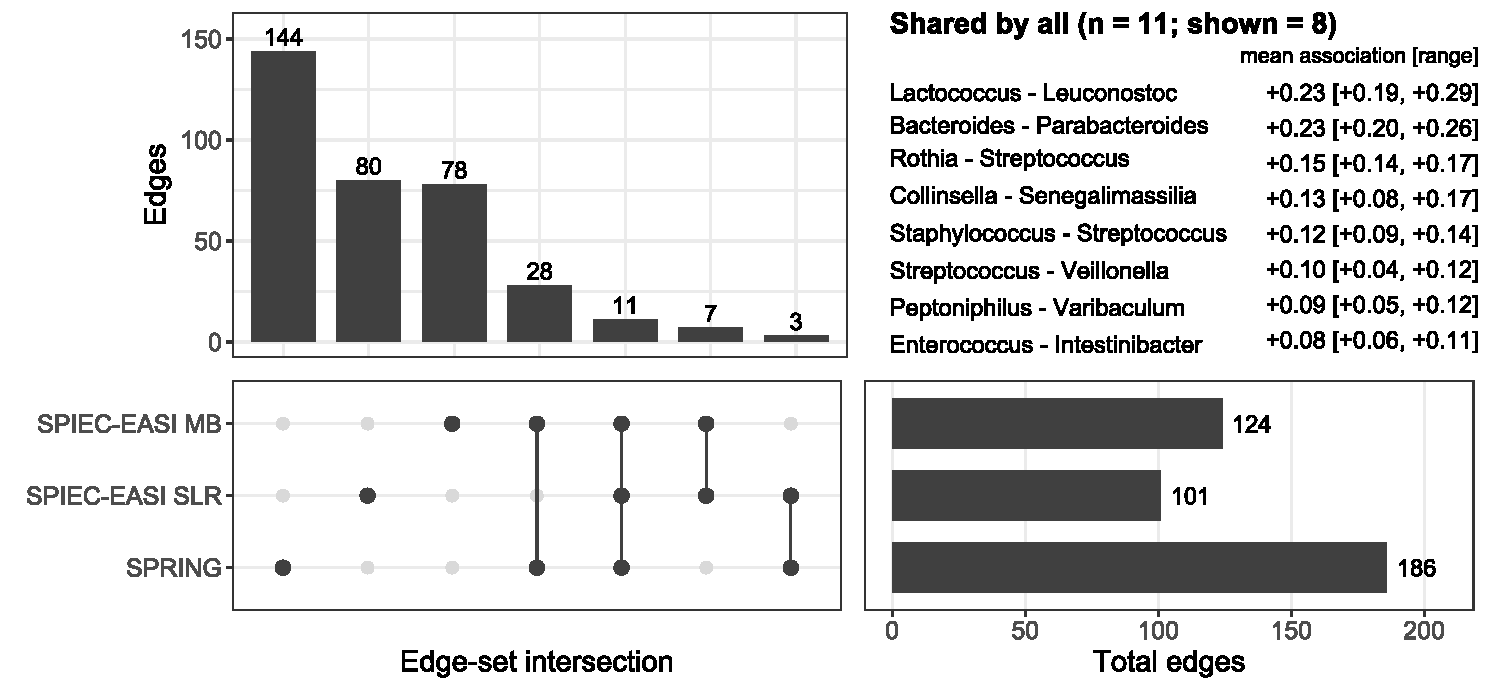
\includegraphics[width=\textwidth]{../ch07_application/figures/10_network_analysis/thesis_edge_upset_association8.pdf}
\caption{\textbf{Shared edges across association estimation methods.} The UpSet plot summarizes overlap among the edge sets estimated by SPIEC-EASI MB, SPIEC-EASI SLR estimation, and SPRING. The upper bar chart shows the number of edges in each intersection, the lower panel indicates the methods contributing to each intersection, and the horizontal bars show the total number of edges in each network. For example, 11 edges are shared among all methods, 3 edges appear only in the SPRING and SLR networks, and 144 only in the SPRING network. The list on the top right shows $8$ of the $11$ edges shared by all three methods, together with their mean estimated association and range across methods.}
\label{fig:7app:network:upset_association}
\end{figure}

Six edges were present in all $8$ networks. Table~\ref{tab:7app:network:persistent_edges} summarizes their estimated association strengths within the three sensitivity-analysis groups and across all selected networks. All six associations are positive, with \emph{Lactococcus}--\emph{Leuconostoc} and \emph{Bacteroides}--\emph{Parabacteroides} showing the largest mean association across the selected networks. The persistence of these edges does not establish their biological origin or imply direct microbial interaction. However, compared with associations that appear only under particular preprocessing or estimation choices, they represent candidate relationships that are less sensitive to the methodological variations considered here.

\begin{table}[!htb]
	\centering
	\caption{\textbf{Edges persistent across sensitivity analyses.} The table lists taxon pairs connected in all eight signed networks considered across prevalence-filtering, zero-replacement, and association-estimation sensitivity analyses. Entries are mean estimated associations within the respective analysis group and across all eight networks.}
	\label{tab:7app:network:persistent_edges}
	\vspace{0.5em}
	\small
	\begin{tabularx}{\textwidth}{l l c c c c}
		\toprule
		Taxon 1 & Taxon 2 & Prevalence filter & Zero repl. & Association & Overall \\
		\midrule
		\emph{Bacteroides} & \emph{Parabacteroides} & $0.20$ & $0.19$ & $0.23$ & $0.208$ \\
		\emph{Rothia} & \emph{Streptococcus} & $0.13$ & $0.13$ & $0.15$ & $0.138$ \\
		\emph{Streptococcus} & \emph{Veillonella} & $0.11$ & $0.11$ & $0.10$ & $0.104$ \\
		\emph{Collinsella} & \emph{Senegalimassilia} & $0.08$ & $0.09$ & $0.13$ & $0.101$ \\
		\emph{Staphylococcus} & \emph{Streptococcus} & $0.08$ & $0.10$ & $0.12$ & $0.100$ \\
		\emph{Gemella} & \emph{Streptococcus} & $0.05$ & $0.05$ & $0.03$ & $0.044$ \\
		\bottomrule
	\end{tabularx}
\end{table}

%%%%%%%%%%%%%%%%%%%%%%%%%%%%%%%%%%%%%
\section{Network comparison between EBF groups}
\label{sec:7app:network}
%%%%%%%%%%%%%%%%%%%%%%%%%%%%%%%%%%%%%

The preceding section examined the sensitivity of a single network estimated from the complete data set to sparsity, zero handling, and association-estimation choices. We now turn to the comparison of association networks estimated separately for children without EBF (``non-EBF'' group) and children with an EBF duration of at least two months (``EBF'' group). This extends the comparative analyses presented in the preceding sections from marginal community- and feature-level differences to differences in estimated association structure. As in the single-network analysis, we revisit genera that were identified as differentially abundant, showed differential distributions, or had high mean CLR coordinates to examine whether they are also involved in differential associations between the two EBF groups. Beyond such taxon- and edge-specific patterns, we investigate whether local or global network characteristics differ significantly between the groups.

The group-specific network analyses were based on the default analysis data set defined in Section~\ref{sec:7app:default_data}, comprising $179$ children in the non-EBF group and $375$ children in the EBF group. As in the preceding network analyses, all networks were estimated at genus level after applying the $1\%$ prevalence filter.

%====================================
\subsection{Descriptive comparison}
\label{sec:7app:network:comparison}
%====================================

Several network-construction approaches were considered. These included SPIEC-EASI MB with Bayesian-multiplicative replacement, SPIEC-EASI sparse-plus-low-rank (SLR) estimation, and SPRING. These three approaches were already considered for the complete data set and yielded networks in which highly sparse genera were less prominently connected than in the baseline SPIEC-EASI MB network based on multiplicative replacement. They are therefore plausible candidates for the subsequent group comparison. For these three methods, the same configuration as in the preceding sections was used. In particular, the regularization path comprised $30$ candidate $\lambda$ values, StARS was based on $30$ subsamples with a stability threshold of $0.1$, and SPIEC-EASI SLR used rank $r=2$, as selected in the analysis of the complete data set.

In addition, correlation shrinkage (cf. Section~\ref{sec:5net:net_constr:sparse_cov_est}) and proportionality shrinkage (cf. Section~\ref{sec:5net:net_constr:prop_shrink}) were considered because shrinkage-based estimators have been reported to be more stable across different sample sizes than several non-shrinkage association estimators \citep{badri2020shrinkage}. Correlation shrinkage was applied to CLR-transformed data, whereas proportionality shrinkage was applied directly to the corresponding zero-replaced compositions. Both approaches were evaluated after either multiplicative replacement (MultRepl) or Bayesian-multiplicative replacement (BayesMultRepl). Because shrinkage estimators generally yield dense association matrices, additional thresholding was used to obtain sparse networks with edge densities comparable to those of the SPIEC-EASI and SPRING networks. Based on the empirical distributions of the estimated associations, an absolute association threshold of $0.3$ was used for networks based on MultRepl and a threshold of $0.15$ for networks based on BayesMultRepl.

Figure~\ref{fig:7app:network:comparison_collection} provides an initial visual comparison of selected group-specific networks. The two SPIEC-EASI approaches and SPRING are displayed in the left panels, and three shrinkage approaches on the right side. Proportionality shrinkage with MultRepl is not shown here, but has a structure similar to that obtained with correlation shrinkage and MultRepl (see also Table~\ref{tab:7app:network:global_measures_comparison}). Labels are omitted because the purpose of this figure is to compare the overall network structures rather than to interpret individual associations. Within each method, the same force-directed layout was used for the two EBF groups. Layouts are the same within one approach, but differ between approaches to preserve the visual network structure within one construction method. In all cases, the repulsion parameter was set to $0.9$ to support broadly comparable visual spacing between nodes.

The overall structure of the SPIEC-EASI SLR and SPRING networks is consistent with the corresponding single-network analyses in the preceding section: both methods yield numerous negative associations, whereas the SLR networks are generally denser than the SPRING networks. In addition, both SPIEC-EASI approaches show a pronounced difference in density between the two EBF groups: the non-EBF networks are substantially denser than the corresponding EBF networks.

Such a pattern can generally arise when networks are constructed from groups of different sample sizes. For a correlation estimator followed by fixed-threshold sparsification, estimates in the smaller group are more variable around their population values, making it more likely that some estimated associations exceed the threshold in absolute value \citep{fisher1921probable}. The present SPIEC-EASI analyses do not use fixed-threshold sparsification, but select the regularization level by StARS. Thus, the preceding argument does not directly imply the observed density difference. Nevertheless, neither SPIEC-EASI nor SPRING can generally be assumed to yield directly comparable network densities when the group sizes differ substantially like in this analysis.

This motivated the additional consideration of correlation and proportionality shrinkage. When used after MultRepl, both shrinkage approaches again produced connected regions dominated by low-abundance genera, indicating that shrinkage alone does not resolve the sensitivity to zero replacement observed in the preceding section. However, the overall connectivity was more similar between the two EBF groups than for the SPIEC-EASI MB networks. We therefore repeated the shrinkage-based analyses using BayesMultRepl. Under both correlation and proportionality shrinkage, the EBF network was then denser than the non-EBF network. Note that these observations are purely descriptive and should not be interpreted as evidence that the shrinkage approaches are generally robust to unequal group sizes, because the true underlying network structures are unknown and no systematic simulation study was conducted in the present analysis.

\begin{figure}[!htb]
\centering
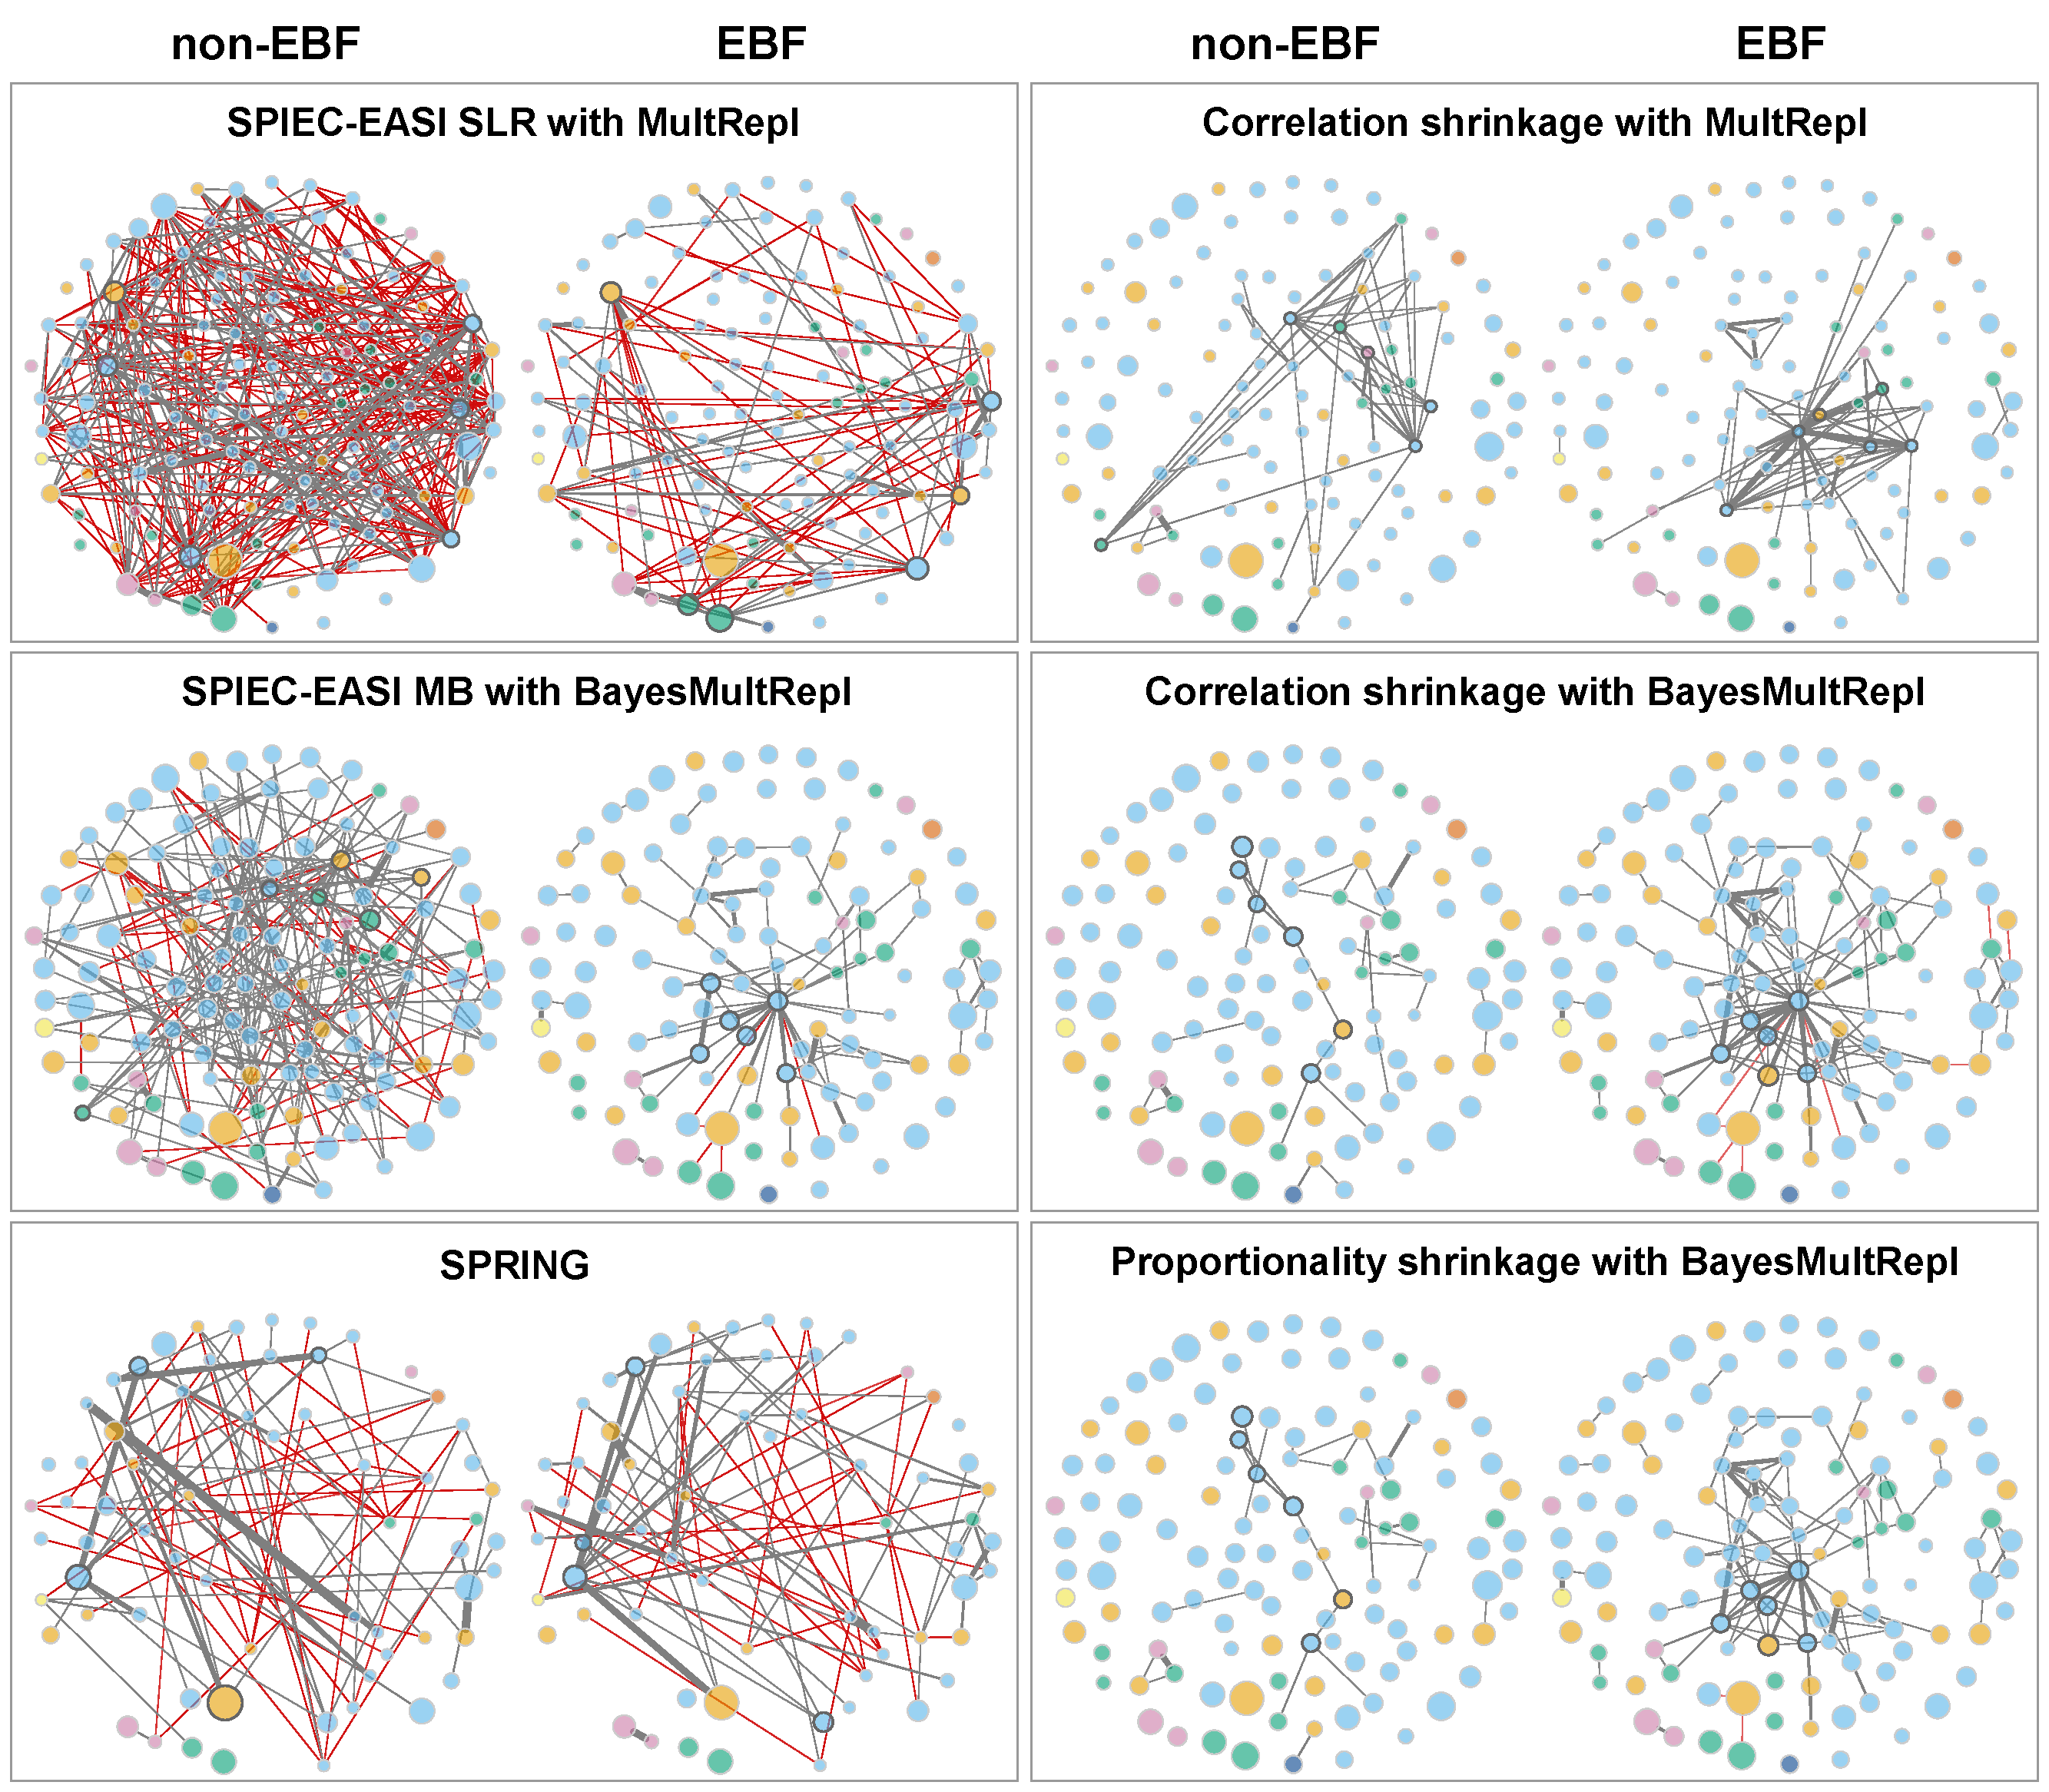
\includegraphics[width=\textwidth]{../ch07_application/figures/11_network_comparison/thesis_combined_networks.pdf}
\caption{\textbf{Group-specific association networks estimated with selected construction approaches.} Networks were estimated separately for non-EBF group ($n=179$) and the EBF group ($n=375$). The displayed approaches are SPIEC-EASI MB with Bayesian-multiplicative replacement (BayesMultRepl), SPIEC-EASI sparse-plus-low-rank (SLR) estimation, SPRING, correlation shrinkage with multiplicative replacement, proportionality shrinkage with BayesMultRepl, and correlation shrinkage with BayesMultRepl. Nodes represent genera and are colored according to phylum, with color coding analogous to Figures~\ref{fig:7app:network:baseline_network} and \ref{fig:7app:network:spiecEasi_slr_unsigned_net}. Node sizes are proportional to the mean CLR coordinate within the respective EBF group. Gray and red edges indicate positive and negative estimated associations, respectively. Labels are omitted to emphasize overall network structure. Within each method, node positions were determined using a common force-directed layout for both EBF groups, with repulsion parameter $0.9$.}
\label{fig:7app:network:comparison_collection}
\end{figure}

Table~\ref{tab:7app:network:global_measures_comparison} summarizes selected global network characteristics for all construction approaches. The relative size of the largest connected component, edge density, and natural connectivity reflect the visual differences in network structure. Across the shrinkage-based approaches, the EBF duration $\geq 2$ group generally has a larger largest connected component (LCC), higher edge density, and greater natural connectivity than the EBF duration $=0$ group. The opposite pattern is observed for the two SPIEC-EASI networks, for which all three network properties are larger in the EBF duration $=0$ group. For SPRING, the corresponding values are broadly similar between groups. These findings mirror the visual impressions from the network plots and demonstrate that apparent group differences in network connectivity depend strongly on the complete network-construction pipeline. Formal comparison of a selected network-construction approach using statistical tests is therefore considered in the following subsection.


\begin{table}[!htb]
\centering
\caption{\textbf{Selected global properties of group-specific association networks.} The table summarizes the relative size of the largest connected component (LCC), edge density, and natural connectivity for networks estimated separately in the two EBF groups. These measures are part of \texttt{NetCoMi}'s analysis summary. Within each method and network property, the larger of the two group-specific values is shown in bold.}
\label{tab:7app:network:global_measures_comparison}
\vspace{0.5em}
\small
\setlength{\tabcolsep}{2.5pt}
\renewcommand{\arraystretch}{1.05}
\begin{tabular}{p{2cm} *{7}{>{\centering\arraybackslash}p{1.7cm}}}
\toprule
& \multicolumn{1}{c}{MB} & \multicolumn{1}{c}{SLR} & \multicolumn{1}{c}{SPRING} & \multicolumn{2}{c}{Cor. shrinkage} & \multicolumn{2}{c}{Prop. shrinkage} \\
\cmidrule(lr){2-2}\cmidrule(lr){3-3}\cmidrule(lr){4-4}\cmidrule(lr){5-6}\cmidrule(lr){7-8}
& BayesMult & MultRepl & -- & MultRepl & BayesMult & MultRepl & BayesMult \\
\midrule
\multicolumn{8}{l}{\textit{Relative LCC size}} \\
non-EBF & $\mathbf{0.983}$ & $\mathbf{0.641}$ & $\mathbf{0.938}$ & $0.145$ & $0.068$ & $0.128$ & $0.068$ \\
EBF & $0.513$ & $0.368$ & $0.892$ & $\mathbf{0.265}$ & $\mathbf{0.650}$ & $\mathbf{0.214}$ & $\mathbf{0.402}$ \\
\addlinespace
\multicolumn{8}{l}{\textit{Edge density}} \\
non-EBF & $\mathbf{0.033}$ & $\mathbf{0.046}$ & $0.041$ & $0.008$ & $0.005$ & $0.006$ & $0.004$ \\
EBF & $0.014$ & $0.015$ & $\mathbf{0.046}$ & $\mathbf{0.012}$ & $\mathbf{0.023}$ & $\mathbf{0.010}$ & $\mathbf{0.017}$ \\
\addlinespace
\multicolumn{8}{l}{\textit{Natural connectivity}} \\
non-EBF & $\mathbf{0.011}$ & $\mathbf{0.013}$ & $0.018$ & $0.010$ & $0.009$ & $0.010$ & $0.009$ \\
EBF & $0.010$ & $0.010$ & $\mathbf{0.019}$ & $\mathbf{0.012}$ & $\mathbf{0.011}$ & $\mathbf{0.012}$ & $\mathbf{0.011}$ \\
\bottomrule
\end{tabular}
\end{table}

%====================================
\subsection{Defining the network construction approach}
\label{sec:7app:network:comparison:approach}
%====================================

The preceding subsection made clear that the visual contrast between the two EBF-group networks can not be seen as a fixed feature of the data, but changes with the network-construction pipeline. Its purpose was therefore not to interpret these plots as evidence of differential network structure, but to identify a construction approach that remains reasonably comparable despite the markedly unequal group sizes. We first motivate the selected association measure and preprocessing strategy for the permutation procedure. Building on this choice, the following sections examine whether the two EBF groups differ in global network structure, node-level properties, or individual associations.

Based on the former comparison, correlation shrinkage with Bayesian-multiplicative replacement was selected for the formal analyses. The shrinkage-based networks showed less pronounced differences in overall connectivity between the two EBF groups than the SPIEC-EASI networks, and Bayesian-multiplicative replacement avoided the highly connected subnetworks of low-abundance genera observed when correlation or proportionality shrinkage was combined with multiplicative replacement. Correlation shrinkage was preferred over proportionality shrinkage because the estimated correlations can additionally be compared between groups using Fisher's $z$-test. This provides an edge-wise complement to the permutation-based approach for differential association analysis.

SPRING was also considered a suitable candidate because its modified CLR transformation avoids external zero replacement. However, network construction could not be completed successfully for a substantial number of permuted group allocations, even after considerably stricter prevalence filtering. In these cases, the fitted model returned missing association estimates. A permutation analysis would then require a principled treatment of failed model fits in the null distribution, including a definition of the test statistic when one or both group-specific networks cannot be estimated. This methodological issue is beyond the scope of the present application.

The SPIEC-EASI MB and SLR approaches were not selected because both produced substantially denser networks for the smaller EBF duration $=0$ group. Although unequal densities do not preclude a formal network comparison, they complicate the interpretation of differences in global and local network properties when the groups differ markedly in sample size. For the SLR approach, this concern was accompanied by a comparatively large number of negative estimated associations. We therefore did not pursue these methods for the formal comparison.

A further decision concerned the role of Bayesian-multiplicative replacement in the permutation procedure. This replacement method estimates prior parameters from the samples included in the data set to which it is applied. Repeating replacement separately within each permuted group would therefore change the group-specific priors and the resulting replacement values after every relabeling. In that formulation, zero replacement forms part of the group-specific network-construction procedure and must be repeated for each permutation.

In the present data set, however, separate Bayesian-multiplicative replacement failed for some permuted group allocations because of the extreme sparsity of the count matrix. We therefore applied Bayesian-multiplicative replacement once to the complete, globally filtered data set before splitting the samples into the observed or permuted EBF groups. The resulting positive composition matrix was treated as a fixed sample representation throughout the permutation procedure, whereas correlation estimation, network construction, and calculation of the respective comparison statistics were repeated after each permutation.

This defines the target of inference as differences between networks estimated from a common Bayesian-multiplicative representation of all samples, rather than differences after separately estimated group-specific replacement models. This choice is coherent because the two EBF groups are subsets of the same cohort and are measured on a common feature table, rather than representing separate sequencing experiments with potentially distinct detection limits. Joint preprocessing also avoids introducing differences in the estimated replacement prior solely through the permutation of group labels.

%====================================
\subsection{Permutation procedure}
\label{sec:7app:network:comparison:permutation}
%====================================

Permutation testing was implemented using the \texttt{createAssoPerm()} function in \texttt{NetCoMi}. This function generates association matrices for permuted group allocations and stores them for subsequent reuse. The resulting matrices can be supplied to \texttt{netCompare()} for testing differences in global and node-level network properties and to \texttt{diffnet()} for testing differential associations. Storing the permuted association matrices ensures that all downstream tests are based on the same set of permuted group allocations and avoids repeated association estimation for each individual comparison statistic.

A further practical advantage of this workflow is that the association matrices can be generated in separate blocks of permutations. This was necessary in the present analysis because generating and storing all permuted matrices simultaneously exceeded the available memory capacity. We therefore performed the permutation procedure in blocks of $20$ permutations. These blocks were computed in parallel, and a separate seed was used for each repetition to ensure reproducibility of the complete permutation procedure. A total of $999$ permutations was generated, consistent with the permutation analyses in the preceding application sections.

The stored permutation matrices were subsequently reused by \texttt{netCompare()} to test differences in global and node-level network properties. As described in Chapter~\ref{ch:netcomi}, we refer to this analysis as ``differential network analysis''. For each test statistic, three $p$-values were considered: the empirical permutation $p$-value, the unconstrained \texttt{permApprox}-refined $p$-value, and the constrained \texttt{permApprox}-refined $p$-value. The results are presented in the following subsection.

The same permutation matrices were then used in \texttt{diffnet()} to test individual differential associations between the EBF groups. In accordance with the terminology introduced in Chapter~\ref{ch:netcomi}, this edge-wise analysis is referred to as ``differential association analysis''. The approach was the same as for the differential network analysis, with the exception that we did not use the default \texttt{permApprox} configuration here, because it led to overly conservative $p$-values compared to the unconstrained ones. We therefore changed the approach to use the maximum of the observed test statistics instead of the permuted ones as saturation cap. In addition we set the tuning parameter to 0.1. The results are presented in Section~\ref{sec:7app:network:comparison:associations}.

The same permutation matrices were then used in \texttt{diffnet()} to test individual differential associations between the EBF groups. In accordance with the terminology introduced in Chapter~\ref{ch:netcomi}, this edge-wise analysis is referred to as ``differential association analysis.'' The analysis followed the same $p$-value refinement strategy as the differential network analysis, but used a modified \texttt{permApprox} configuration. Under the default settings, the constrained \texttt{permApprox} $p$-values were substantially larger than the corresponding unconstrained estimates. We therefore changed the saturation cap to use the maximum of the observed edge-wise test statistics rather than the maximum of the permuted test statistics, and set the tuning parameter to $0.1$. The results are presented in Section~\ref{sec:7app:network:comparison:associations}.

%====================================
\subsection{Differential network analysis}
\label{sec:7app:network:comparison:global}
%====================================

Figure~\ref{fig:7app:network:ebf_network} shows the group-specific correlation-shrinkage networks estimated after Bayesian-multiplicative replacement. A common force-directed layout was used for both networks so that differences in the displayed association structure can be assessed without being confounded by changes in node positions. Like already observed in the descriptive comparison, both networks are sparse and contain several disconnected components. In addition to the general difference in edge density, their local structures also differ visibly in several regions. Most notably, \emph{Coprobacillus} is disconnected in the EBF duration $=0$ network, whereas it is highly connected (to 32 other genera) in the EBF network. These differences in connectivity are also reflected in the degree distributions shown in Figure~\ref{fig:7app:network:ebf_degree_distribution}. The CLR-coordinate heatmap in Figure~\ref{fig:app:7app:net_compare_clr_heatmap} shows that the mean CLR coordinates after Bayesian-multiplicative replacement of \emph{Coprobacillus} are not high compared to other genera but it is also not among the rarest ones. Nevertheless, the possibility that the high connectivity in the EBF network is an artifact of zero handling cannot be dismissed.

\begin{figure}[H]
\centering
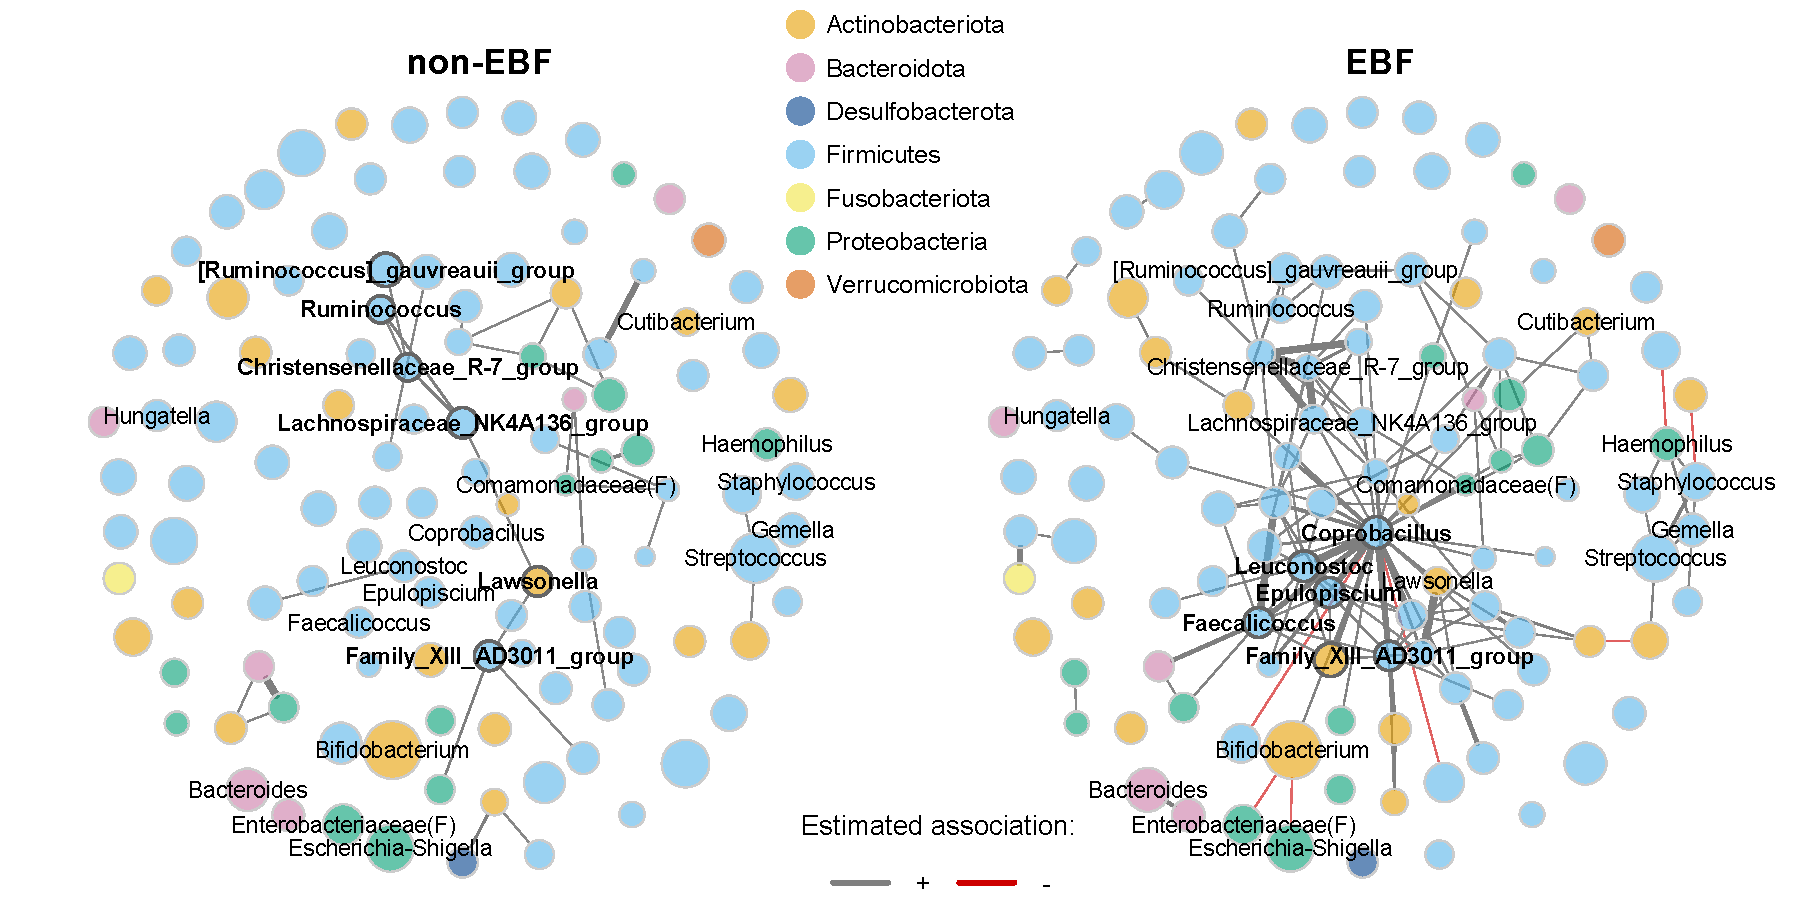
\includegraphics[width=\textwidth]{../ch07_application/figures/11_network_comparison/thesis_ebf_network_plot_same_layout-1.pdf}
\caption{\textbf{Group-specific correlation shrinkage networks.} Networks were estimated separately for the non-EBF and the EBF group, using the approach described in Section~\ref{sec:7app:network:comparison:approach}. Nodes represent genera and are colored according to phylum. Node sizes are proportional to the mean CLR coordinate within the respective EBF group. Gray and red edges indicate positive and negative estimated correlations, respectively. A common force-directed layout was used for both networks to facilitate visual comparison of their association structures. Labels identify genera considered in the preceding differential abundance and differential distribution analyses, together with selected genera highlighted in the network comparison.}
\label{fig:7app:network:ebf_network}
\end{figure}

\begin{figure}[H]
\centering
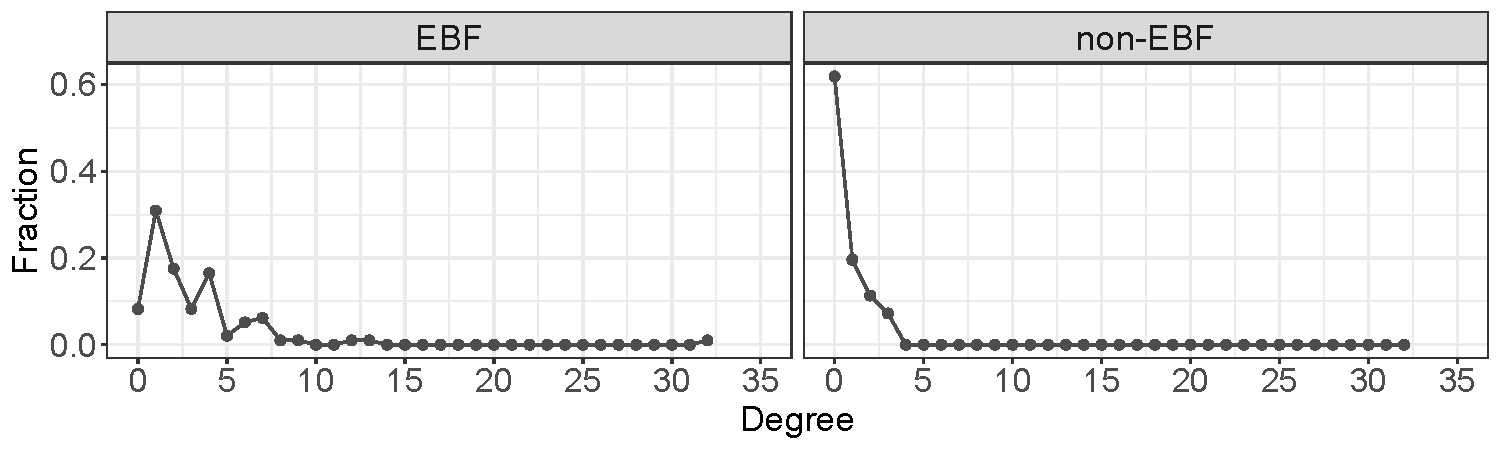
\includegraphics[width=0.9\textwidth]{../ch07_application/figures/11_network_comparison/thesis_ebf_degree_distribution_side_by_side-1.pdf}
\caption{\textbf{Degree distributions of the two EBF networks.} The panels show the distributions of non-normalized node degree for the correlation-shrinkage networks estimated separately for the EBF and non-EBF group. Nodes with degree zero correspond to disconnected genera.}
\label{fig:7app:network:ebf_degree_distribution}
\end{figure}

The \texttt{netCompare()} output, parts of which are shown below, provides further insight into whether the visual differences are reflected in numerical differences between network measures and whether these differences are larger than expected under permutation of the EBF-group labels. For each measure, the output below reports the values in the two groups, their absolute difference, and the empirical permutation $p$-value. No multiple-testing adjustment was applied because the global network properties were interpreted as distinct summary measures rather than as a common family of hypotheses. Refining the $p$-values with \texttt{permApprox} had no effect because all empirical $p$-values exceeded the threshold below which $p$-values were selected for refinement. The upper part of the output contains measures computed for the largest connected component (LCC), whereas the lower part contains measures that are also meaningful for the complete network. None of the tested differences was statistically significant.


\begin{Verbatim}[fontsize=\footnotesize]
Global network properties
`````````````````````````
Largest connected component (LCC):
                         non-EBF    EBF    abs.diff.     $p$-value  
Relative LCC size          0.068  0.650        0.581    0.347000  
Clustering coefficient     0.336  0.440        0.105    0.623000  
Modularity                 0.369  0.535        0.166    0.353000  
Positive edge percentage 100.000 94.558        5.442    0.377000  
Edge density               0.286  0.052        0.234    0.210000  
Natural connectivity       0.192  0.019        0.173    0.133000  
Vertex connectivity        1.000  1.000        0.000    1.000000  
Edge connectivity          1.000  1.000        0.000    1.000000  
Average dissimilarity*     0.895  0.981        0.086    0.207000  
Average path length**      1.744  2.458        0.715    0.361000  

Whole network:
                         non-EBF    EBF    abs.diff.     $p$-value  
Number of components      90.000 35.000       55.000    0.262000  
Clustering coefficient     0.408  0.433        0.025    0.908000  
Modularity                 0.840  0.565        0.275    0.443000  
Positive edge percentage 100.000 94.805        5.195    0.259000  
Edge density               0.005  0.023        0.018    0.461000  
Natural connectivity       0.009  0.011        0.002    0.543000  
-----
$p$-values: one-tailed test with null hypothesis diff=0
 *: Dissimilarity = 1 - edge weight
**: Path length = Units with average dissimilarity
\end{Verbatim}

The following output shows the graphlet correlation distances (GCD) in the two groups, which provides a complementary comparison of the local topological organization of the networks. In contrast to the preceding global summary measures, it quantifies the overall discrepancy between the graphlet correlation matrices (GCMs) of the two networks. Appendix Figure~\ref{fig:app:7app:net_compare_gcm} shows the corresponding GCM heatmaps, including significance codes resulting from Fisher's z tests.

\begin{Verbatim}[fontsize=\footnotesize]
Graphlet Correlation Distance
`````````````````````````````
        wholeNet         LCC  
GCD        2.372       4.221  
$p$-value 0.161000    0.300000  
-----
GCD >= 0 (GCD=0 indicates perfect agreement between GCMs)
$p$-value: permutation test with null hypothesis GCD=0
\end{Verbatim}

The estimated GCD was $2.372$ for the complete networks and $4.221$ for their largest connected components. Neither value was statistically significant under permutation of the EBF-group labels. Thus, although Fisher's $z$-tests indicated differences for several individual GCM entries, the aggregate difference in graphlet correlation structure was not larger than expected under the permutation null distribution. 

The node-level comparison similarly revealed several descriptive contrasts, particularly for genera that were disconnected in one network but embedded in a connected component in the other. The \texttt{netCompare()} output below lists the centrality measures with the smallest unadjusted permutation $p$-values. The output shows for genus the centrality values in the two groups, their absolute difference, as well as the empirical $p$-values before and after adjustment for multiplicity. The \texttt{permApprox}-refined $p$-values were almost identical to the empirical $p$-values because none of the $p$-values was below the minimum attainable empirical $p$-value for $999$ permutations. Consequently, $p$-value refinement did not affect any inferential decision.

\begin{Verbatim}[fontsize=\footnotesize]
Centrality measures
- In increasing order of unadjusted $p$-values
````````````````````````````````````````````````
Degree (unnormalized):
               non-EBF EBF abs.diff.  $p$-value     adj.$p$-value  
Leuconostoc          0  13        13 0.016000 *      1.000000  
Lactobacillus        0   1         1 0.042000 *      1.000000  
Staphylococcus       0   4         4 0.043000 *      1.000000  
Coprobacillus        0  32        32 0.048000 *      1.000000  
Gemella              0   4         4 0.080000 .      1.000000  

Betweenness centrality (unnormalized):
              non-EBF  EBF abs.diff.  $p$-value     adj.$p$-value  
Rothia              0  536       536 0.002000 **     0.156000  
Varibaculum         0  594       594 0.003000 **     0.156000  
Coprobacillus       0 1936      1936 0.004000 **     0.156000  
Peptoniphilus       0  610       610 0.007000 **     0.204750  
Streptococcus       0  478       478 0.015000 *      0.351000  

Closeness centrality (unnormalized):
              non-EBF    EBF abs.diff.  $p$-value     adj.$p$-value  
Lactobacillus       0 16.938    16.938 0.042000 *      0.715565  
Leuconostoc         0 59.065    59.065 0.083000 .      0.715565  
Coprobacillus       0 76.861    76.861 0.095000 .      0.715565  
Eggerthella         0 18.573    18.573 0.136000        0.715565  
Epulopiscium        0 53.335    53.335 0.144000        0.715565  

Eigenvector centrality (unnormalized):
                 non-EBF   EBF abs.diff.  $p$-value     adj.$p$-value  
Ruminococcus       0.821 0.007     0.814 0.020000 *      0.959400  
Leuconostoc        0.000 0.639     0.639 0.035000 *      0.959400  
Terrisporobacter   0.000 0.033     0.033 0.037000 *      0.959400  
Coprobacillus      0.000 1.000     1.000 0.037000 *      0.959400  
Lactobacillus      0.000 0.000     0.000 0.041000 *      0.959400  
_________________________________________________________
Significance codes: ***: 0.001, **: 0.01, *: 0.05, .: 0.1
\end{Verbatim}

Before multiplicity adjustment, \emph{Leuconostoc}, \emph{Lactobacillus}, \emph{Staphylococcus}, and \emph{Coprobacillus} showed differences in unnormalized degree, with all four genera having degree zero in the non-EBF network and positive degree in the EBF network. In particular, \emph{Coprobacillus} had degree $32$ in the latter network, consistent with its visually prominent local position in Figure~\ref{fig:7app:network:ebf_network}. Several genera, including \emph{Rothia}, \emph{Varibaculum}, \emph{Coprobacillus}, and \emph{Peptoniphilus}, also had comparatively small unadjusted $p$-values for betweenness centrality.

However, none of the node-level differences remained statistically significant after Benjamini--Hochberg adjustment across genera. The observed centrality contrasts should therefore be interpreted as descriptive patterns rather than as confirmed differential node properties. 

Taken together, the differential network analysis does not provide evidence for global or node-level differences that are robust to the multiplicity adjustment applied here, despite the visible differences between the two estimated networks.

%====================================
\subsection{Differential association analysis}
\label{sec:7app:network:comparison:associations}
%====================================

After comparing the two EBF-group networks at the level of overall network properties, we next examined whether individual associations differed between the groups. This edge-wise analysis was based on the same correlation-shrinkage approach after Bayesian-multiplicative replacement that was used for the differential network analysis. For each of the $\binom{117}{2}=6786$ possible genus pairs, the difference between the two group-specific association estimates was tested by permutation using the precomputed permuted association matrices. Thus, in contrast to an analysis restricted to edges that are non-zero in at least one of the observed networks, the present analysis follows the stricter approach of testing all possible edges in parallel. This leads to a particularly severe multiplicity burden after Benjamini--Hochberg adjustment, but avoids conditioning the tested hypotheses on the observed sparsified networks.

Figure~\ref{fig:7app:network:diffassoc_pvalues} compares the raw empirical permutation $p$-values with the corresponding \texttt{permApprox}-refined $p$-values. The y-axis shows the unadjusted $p$-values, whereas colored points indicate edges that were significant after Benjamini--Hochberg adjustment. As expected from $999$ permutations, the empirical $p$-values are bounded below by $1/(999+1)=0.001$, so the empirical analysis cannot distinguish among the strongest signals. In contrast, the \texttt{permApprox} refinement yields a much more informative ranking of small $p$-values. The unconstrained approximation produced one $p$-value equal to zero, whereas the constrained approximation avoided this artifact and returned finite tail $p$-values throughout. In this example, the unconstrained and constrained results are very similar for most edges, and the constrained approach is only slightly more conservative. In the plot, edges for which the constrained and unconstrained $p$-values were nearly identical are highlighted in yellow, whereas other colors mark edges whose refined $p$-values changed more visibly under the constraint.

\begin{figure}[!htb]
\centering
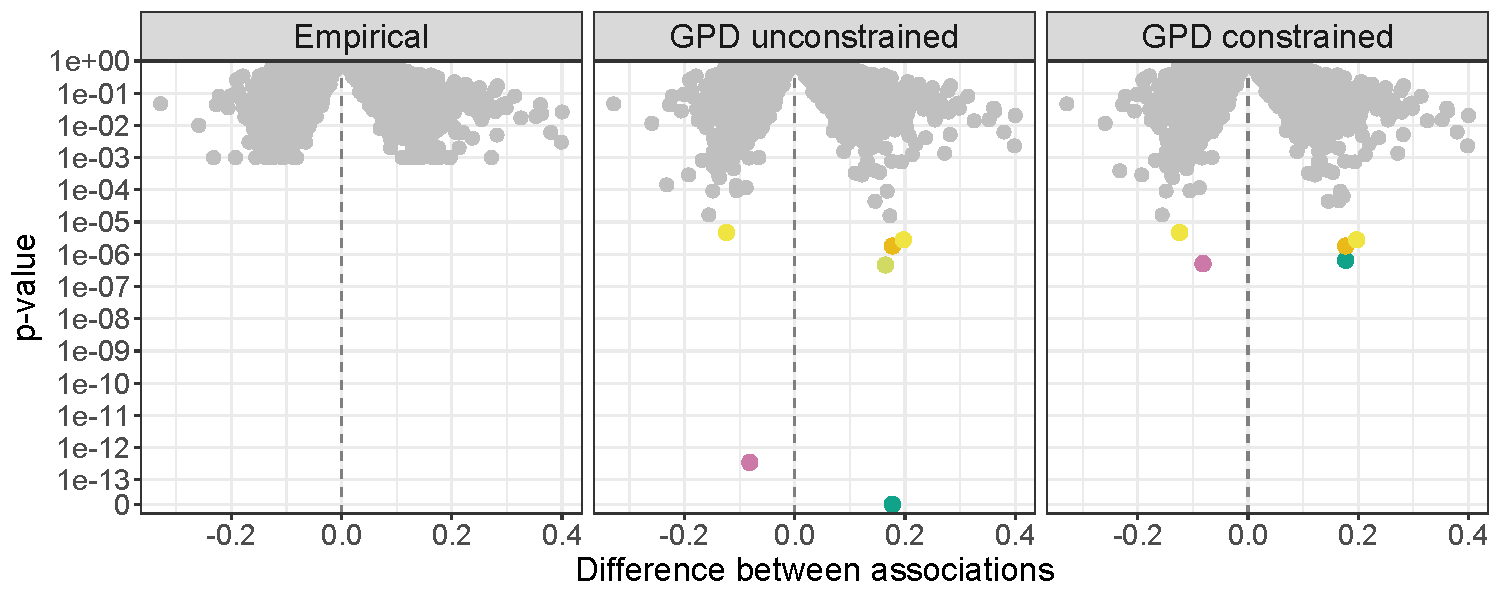
\includegraphics[width=\textwidth]{../ch07_application/figures/11_network_comparison/thesis_diffnet_raw_pvalue_comparison-1.pdf}
\caption{\textbf{Comparison of empirical and \texttt{permApprox}-refined $p$-values for differential associations.} Each point represents one tested genus pair. The y-axis shows the unadjusted $p$-value, and point colors indicate whether the edge was significant after Benjamini--Hochberg adjustment at $\alpha = 5\%$. Because the empirical permutation analysis is based on $999$ permutations, empirical $p$-values are bounded below by $0.001$. The \texttt{permApprox} refinement yields continuous tail $p$-values below this bound. Yellow points indicate genus pairs for which the unconstrained and constrained \texttt{permApprox} $p$-values were nearly identical, whereas other colors highlight more noticeable differences between the two approximations.}
\label{fig:7app:network:diffassoc_pvalues}
\end{figure}


Table~\ref{tab:7app:network:diffassoc_pvalues} lists the raw $p$-values for the edges with the smallest unconstrained \texttt{permApprox} $p$-values. The strongest signals are concentrated in a small set of genera. In particular, several edges involve the cluster around \emph{Streptococcus}, \emph{Staphylococcus}, \emph{Gemella}, and \emph{Haemophilus}, which already stood out in the group-specific network plots. The association between \emph{Gemella} and \emph{Streptococcus} is the most extreme example: its empirical $p$-value is again limited to $0.001$, whereas the unconstrained approximation yields a $p$-value of zero and the constrained approximation still gives a very small but finite value. Other prominent edges include \emph{Hungatella}--\emph{Cutibacterium}, \emph{Scardovia}--\emph{Cutibacterium}, and \emph{[Eubacterium] coprostanoligenes group}--\emph{Lactococcus}.

\begin{table}[!htb]
\centering
\caption{\textbf{Raw $p$-values for selected differential associations.} The table lists the genus pairs with the smallest unconstrained \texttt{permApprox} $p$-values in the differential association analysis, ordered by increasing unconstrained $p$-value. $p_{\mathrm{empirical}}$ denotes the empirical permutation $p$-value, whereas $p_{\mathrm{permApprox(U)}}$ and $p_{\mathrm{permApprox(C)}}$ denote the unconstrained and constrained GPD-based \texttt{permApprox} $p$-values, respectively.}
\label{tab:7app:network:diffassoc_pvalues}
\vspace{0.5em}
\small
\setlength{\tabcolsep}{4pt}
\begin{tabular}{llrrrr}
\toprule
Taxon 1 & Taxon 2 & Difference & $p_{\mathrm{empirical}}$ & $p_{\mathrm{permApprox(U)}}$ & $p_{\mathrm{permApprox(C)}}$ \\
\midrule
\emph{Gemella} & \emph{Streptococcus} & 0.17736534 & 1.00e-03 & 0.00e+00 & 6.50e-07 \\
\emph{Hungatella} & \emph{Cutibacterium} & -0.08159082 & 1.00e-03 & 3.45e-13 & 5.12e-07 \\
\emph{Haemophilus} & \emph{Staphylococcus} & 0.16479100 & 1.00e-03 & 4.63e-07 & 4.53e-05 \\
\emph{Haemophilus} & \emph{Streptococcus} & 0.17737423 & 1.00e-03 & 1.80e-06 & 1.80e-06 \\
\emph{Haemophilus} & \emph{Gemella} & 0.19718139 & 1.00e-03 & 2.80e-06 & 2.80e-06 \\
\emph{Leuconostoc} & \emph{Staphylococcus} & -0.12385940 & 1.00e-03 & 4.73e-06 & 4.73e-06 \\
\emph{Staphylococcus} & \emph{Streptococcus} & 0.17278499 & 1.00e-03 & 1.56e-05 & 6.35e-05 \\
\emph{Scardovia} & \emph{Cutibacterium} & -0.15588102 & 1.00e-03 & 1.67e-05 & 1.67e-05 \\
\emph{[Eubacterium] copro.} & \emph{Lactococcus} & 0.14566499 & 1.00e-03 & 4.40e-05 & 4.40e-05 \\
\bottomrule
\vspace{1em}
\end{tabular}
\end{table}

Figure~\ref{fig:7app:network:diffassoc_network} displays the differential association network, which contains edges with significant between-group differences in association. The network uses the same layout as the two group-specific network plots to facilitate comparison. A striking feature is again the \emph{Streptococcus}-centered region on the right-hand side, where several significant differential associations occur among \emph{Streptococcus}, \emph{Staphylococcus}, \emph{Gemella}, and \emph{Haemophilus}. In contrast, several associations that were visually noticeable in the descriptive network plots, such as the negative associations involving \emph{Bifidobacterium}, were not significant in the formal edge-wise comparison. Some significant edges in the differential association network are not visible in the group-specific network plots because the latter were based on sparsified networks, whereas the differential association analysis uses the underlying raw association estimates before thresholding. Thus, the differential association network highlights changes in association strength between the groups even when the individual associations are too weak to appear as edges in the displayed group-specific networks.

\begin{figure}[!htb]
\centering
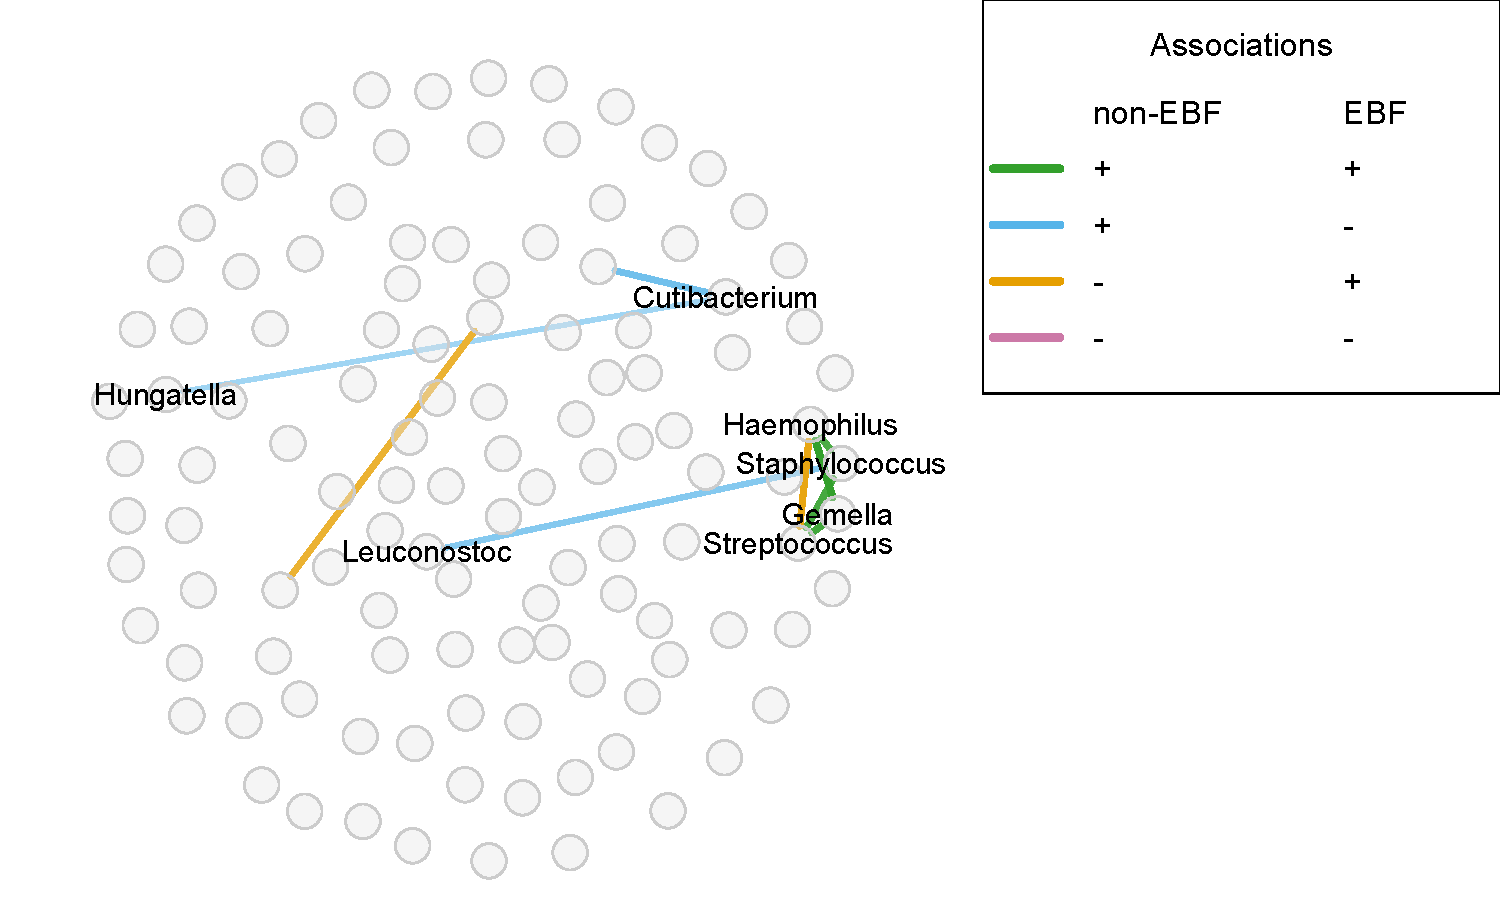
\includegraphics[width=0.9\textwidth]{../ch07_application/figures/11_network_comparison/thesis_ebf_diffnet_plot_same_layout-1.pdf}
\caption{\textbf{Differential association network between the two EBF groups.} Edges represent genus pairs with significant differences in association between children without EBF and children with EBF duration $\geq 2$ months. Edge colors indicate the direction of the association in the two groups. The network uses the same layout as the group-specific network plots to facilitate comparison. Several significant differential associations are concentrated in the \emph{Streptococcus}-centered region, whereas other visually striking associations from the descriptive network plots, such as negative associations involving \emph{Bifidobacterium}, were not significant.}
\label{fig:7app:network:diffassoc_network}
\end{figure}

%%%%%%%%%%%%%%%%%%%%%%%%%%%%%%%%%%%%%
\section{Discussion}
\label{sec:7app}
%%%%%%%%%%%%%%%%%%%%%%%%%%%%%%%%%%%%%

This chapter applied the methodological components developed throughout the thesis to a reduced subset of the PASTURE cohort. The analysis combined community-level summaries, feature-level comparisons, and association-network analyses, using a common genus-level representation where possible while allowing method-specific preprocessing when required. Its primary purpose was to illustrate how these complementary perspectives can be combined in a coherent microbiome workflow, rather than to provide definitive biological conclusions about the effects of breastfeeding in the full PASTURE cohort.

Across the community-level analyses, breastfeeding-related variables emerged as the most consistent sources of variation in the two-month gut microbiome. BF duration and EBF duration were associated with within-sample diversity, between-sample dissimilarity, and mean CLR composition. The analyses also illustrate that these perspectives are related but not interchangeable. The ordination plots did not show clearly separated EBF groups, whereas PERMANOVA, regression-based analyses, and compositional equivalence nevertheless indicated systematic differences when the full multivariate information was used. Thus, the EBF contrast is better interpreted as a gradual shift in community composition than as a division into two distinct microbiome states.

The results further demonstrate the value of distinguishing marginal feature-level effects from broader distributional changes. Differential abundance analysis identified several genera whose relative abundances differed between the EBF groups. \emph{Enterococcus}, \emph{Lactococcus}, \emph{Intestinibacter}, and the \emph{[Ruminococcus] gnavus group} showed higher abundance in children without EBF, whereas \emph{Bifidobacterium} was more abundant in children with EBF duration of at least two months. The latter pattern is consistent with the well-established association between breastfeeding and \emph{Bifidobacterium}-dominated infant gut communities \citep{backhed2015dynamics,stewart2018temporal}.

Differential distribution analysis recovered a partly overlapping set of genera, but additionally distinguished between changes in the distribution among non-zero observations and changes in zero prevalence. This distinction is particularly relevant for sparse microbiome data, where a taxon can differ between groups because of shifts in its positive abundance distribution, because of changes in detection frequency, or through both mechanisms. The agreement between the different feature-level analyses therefore strengthens the interpretation that EBF duration is associated with broad changes in the early gut microbiome, while their differences underline that no single taxon-level method captures all relevant aspects of the data.

The network analyses added a relational perspective to these findings, but also offered strong indications of the sensitivity of microbial network inference to methodological choices. In the complete data set, the apparent prominence of low-abundance genera depended strongly on prevalence filtering, zero replacement, and association estimation. Several edges remained visible across alternative specifications, but the overall network structure and the presence of highly connected taxa changed substantially. This result is not a defect of a particular method; rather, it reflects the limited information available for estimating associations involving sparse taxa. It reinforces the need to interpret microbial association networks as model-dependent summaries of statistical dependence, not as direct reconstructions of ecological interactions.

For the EBF comparison, the selected correlation-shrinkage approach with Bayesian-multiplicative replacement produced group-specific networks that were sufficiently comparable for the subsequent permutation analyses. No robust differences in global network properties or node-level centrality measures were detected after the respective inferential procedures. In contrast, the edge-wise differential association analysis identified several associations that differed between the EBF groups, particularly in the region involving \emph{Streptococcus}, \emph{Staphylococcus}, \emph{Gemella}, and \emph{Haemophilus}. This contrast between largely non-significant global network summaries and significant individual differential associations is not inherently contradictory, because the two analyses target different aspects of network structure and are subject to different multiplicity burdens. The results indicate that the detectable EBF-related differences in the present analysis are concentrated in a limited set of associations, particularly around \emph{Streptococcus}, \emph{Staphylococcus}, \emph{Gemella}, and \emph{Haemophilus}, rather than providing clear evidence for a difference in the selected global network properties. This does not rule out more diffuse structural differences that were not captured by the considered summaries or could not be detected with the available sample sizes and permutation budget.

Permutation-based inference and $p$-value refinement played different roles across the analyses. For tests with moderate $p$-values, empirical permutation inference was adequate and \texttt{permApprox} did not alter the resulting conclusions. Its practical value became most visible when the empirical $p$-value resolution was limiting. In the differential abundance analysis, refinement based on a comparatively small permutation budget yielded a ranking of strong signals that was broadly coherent with a substantially more expensive analysis using $10^7$ permutations. In the differential distribution and differential association analyses, constrained tail approximation avoided zero $p$-values and provided finite, ordered tail probabilities below the empirical resolution limit. These examples illustrate that \texttt{permApprox} is not intended to manufacture significance from weak evidence. Rather, it provides additional resolution when the observed statistic lies in a tail region that cannot be meaningfully distinguished by a limited number of permutations alone.

Several limitations should be kept in mind. First, the analysis is observational and the EBF groups differ in size. The reported associations cannot be interpreted causally, and they may partly reflect correlated early-life exposures, unmeasured confounding, or cohort-specific characteristics. The discrepancy between marginal and adjusted diversity analyses for delivery mode provides a concrete example of this issue. Second, EBF duration was selected as the main grouping variable after inspecting several candidate variables. Although the subsequent analyses were prespecified conditional on this choice, the full workflow should not be interpreted as a single confirmatory analysis with family-wise error control across all exploratory decisions.

\newpage
Third, no universal preprocessing strategy exists for sparse compositional microbiome data. The present analyses necessarily combined methods with different data representations and assumptions: DACOMP used a count-based reference approach, the community-level and network analyses used CLR-based representations, and \texttt{waddR} required an additional adaptation to microbiome data. Bayesian-multiplicative replacement was performed once before the network permutations to obtain a fixed common sample representation. This defines a coherent inferential target for the present cohort, but differs from a procedure in which the replacement model would be re-estimated within every permuted group. Finally, GPD-based $p$-value refinement introduces a fitted tail model and therefore depends on the adequacy of the selected tail approximation. It improves resolution but cannot replace careful diagnostic assessment or larger permutation budgets where feasible, or external replication.

Overall, the PASTURE application illustrates the central message of this thesis: reliable microbiome inference requires attention not only to the final test statistic, but also to the complete chain of data representation, preprocessing, estimation, and inference. The combination of community-level, feature-level, and network-based analyses yielded a more informative picture than any individual method alone. At the same time, the sensitivity analyses show why methodological transparency, robustness checks, and cautious interpretation are indispensable when drawing conclusions from sparse and compositional microbiome data. In the present data set, sparsity was substantial, such that associations and distributional characteristics of many genera were informed by comparatively few non-zero observations. Consequently, results may be sensitive to the handling of excess zeros, including the selected zero-replacement procedure, particularly for network-based analyses. The reported findings should therefore be interpreted as conditional on the employed analytical choices and should not be generalized beyond this cohort without external validation.
